\documentclass[compress,10pt,aspectratio=169]{beamer}

%%%%%%%%%%%%%%%%%%%%%%%
% Thème beamer ONERA :
% Options :
%%%%%%%%%%%%%%%%%%%%%%%
%     - english -> biblio en anglais [défaut en français]
%	  (se sert de la mise en forme bibliographique onera.bst de Frédéric Cassaing (Frederic.Cassaing@onera.fr)
%	  (+url de la page de remerciement renvoie vers le site ONERA en anglais [défaut renvoie sur le site en français]).
%     - customnumbering -> permet d'afficher la numérotation des diapositives de manière élégante.
%	  (/!\ la compilation peut être longue avec cette option si il y a beaucoup de diapositives ! Il vaut mieux alors compiler sans l'option
%	   puis compiler une fois les diapositives finalisées).
%     - DR, CD, SD, S, TS -> ajout de la mention 'DIFFUSION RESTREINTE' ou 'CONFIDENTIEL DEFENSE' ou 'SECRET DEFENSE' ou 'SECRET' ou 'TRES SECRET'(rouge) dans le footer de la présentation. (Note, il ne faut choisir qu'une seule mention à la fois!)
%     - SF -> ajout de la mention 'SPECIAL FRANCE' (bleu) dans le footer de la présentation
%\usetheme[customnumbering]{onera}
\usetheme[english]{onera}


%%%%%%%%%%%%%%%%%%%%%%%
% Packages additionnels
%%%%%%%%%%%%%%%%%%%%%%%
\usepackage{amsmath,amssymb,amsfonts}
\usepackage{stmaryrd}
\usepackage{multirow}
\usepackage{bbold}
\usepackage{epsfig}
\usepackage{ulem}
\usepackage{comment}
\newcommand{\thicktilde}[1]{\mathbf{\tilde{\text{$#1$}}}}


\usepackage{algorithm2e}
\renewcommand{\listalgorithmcfname}{Liste des Algorithmes}%
\renewcommand{\algorithmcfname}{Algorithme}%
\renewcommand{\algorithmautorefname}{algorithme}%
\renewcommand{\algorithmcflinename}{ligne}%
%\renewcommand{\algocf@typo}{\ }%
%\renewcommand{\@algocf@procname}{Proc\'edure}%
%\renewcommand{\@algocf@funcname}{Fonction}%
\renewcommand{\procedureautorefname}{proc\'edure}%
\renewcommand{\functionautorefname}{fonction}%
%\renewcommand{\algocf@languagechoosen}{french}%

%\SetKwHangingKw{HDonnees}{Donnees$\rightarrow$}
%\SetKwInpsut{Donnees}{Donn\'ees}%
%\SetKwInput{Res}{R\'esultat}%
\SetKwInput{Entrees}{Entr\'ees}%
\SetKwInput{Entree}{Entr\'ees}%
\SetKwInput{Sortie}{Sortie}%
\SetKwInput{Sorties}{Sorties}%
%\SetKw{KwA}{\`a}%
%\SetKw{Retour}{retourner}%
%\SetKwBlock{Deb}{d\'ebut}{fin}%
\SetKwRepeat{Repeter}{r\'ep\'eter}{jusqu'\`a}%
%
\SetKwIF{Si}{SinonSi}{Sinon}{si}{alors}{sinon si}{sinon}{fin si}%
\SetKwSwitch{Suivant}{Cas}{Autre}{suivant}{faire}{cas o\`u}{autres cas}{fin cas}{fin d'alternative}%
\SetKwFor{Pour}{pour}{faire}{fin pour}%
\SetKwFor{PourPar}{pour}{faire en parall\`ele}{fin pour}%
\SetKwFor{PourCh}{pour chaque}{faire}{fin pour chaque}%
\SetKwFor{PourTous}{pour tous}{faire}{fin pour tous}%
\SetKwFor{Tq}{tant que}{faire}{fin tq}%


% Dessin (Note : le package 'tikz' est chargé par défaut avec le thème ONERA ainsi que l'option 'positioning')
\usepackage{tikz-3dplot}
\usetikzlibrary{shapes.misc}
\tikzset{cross/.style={cross out, draw=black, fill=none, minimum size=2*(#1-\pgflinewidth), inner sep=0pt, outer sep=0pt}, cross/.default={2pt}}

%%%%%%%%%%%%%%%%%%%%%%%
% Définition de la page de titre %%%%%  A COMPLETER OU IL Y A DEJA DU TEXTE !!!   %%%%%%
%%%%%%%%%%%%%%%%%%%%%%%

\title[]{Generation of structured block quadrilateral meshes from cross fields\vspace{0.5cm}}
\subtitle[]{JSO Jeroboam/LMA2S, Toulouse, France\vspace{0.5cm}}
\author[]{\underline{Kokou Dotse}%\inst{1,*}
, Vincent Mouysset
%\inst{1}
and Sébastien Pernet
%\inst{1}
%\\*\href{mailto:kokou.dotse@onera.fr}{\texttt{kokou.dotse@onera.fr}}
}
%\date[15 Mars 2023]{15 Mars 2023}
\date[]{}
\directors{}
\encadrant{}
%\encadrant{Vincent Mouysset(DTIS/MACI)\textsuperscript{1}}
\grant{}
\tutor{} % D'autres personnes importantes (DGA etc.)
%\institute{\inst{1}ONERA The French Aerospace Lab, Toulouse, France}
\logoUn{} %N'apparaît que si est rempli
\logoDeux{} %N'apparaît que si est rempli




%%%%%%%%%%%%%%%%%%%%%%%%%%%%%%%%%%%%%%%%%%
% Début du document
\begin{document}

% Page de titre (optionnel) %
\MakeTitlePage

%\graphicspath{{../img//}}

%%%%%%%%%%%%%%%%%
% CORPS DE LA PRESENTATION %
%%%%%%%%%%%%%%%%%


\begin{frame}
\frametitle{Context}
\small
\begin{columns}
    \begin{column}{0.8\textwidth}
    \vspace{-0.3cm}
\begin{itemize}
\item {\color{onera} Meshing:} discretization into elementary cells, essential for numerical simulations (fluid mechanics, electromagnetism, etc.). Triangular meshes ("mesh tri") have been well developed for over half a century. Generating good quadrilateral meshes ("mesh quad") remains complex.\\\vspace{0.25cm}

\item {\color{onera} Quadrilateral meshes ("mesh quad"):} these offer excellent properties for various schemes (FD, FEM, SD, DG, etc.).\\\vspace{0.2cm}

\item {\color{onera} Structured:} low storage, optimized for parallel computation.\\\vspace{0.2cm}

\item {\color{onera} Tensor nature:} suitable for order increase, quadrature, sparse systems.\\\vspace{0.2cm}

\item {\color{onera} Anisotropic stretching:} boundary layer meshing, capturing strong variations.\\\vspace{0.25cm}
\end{itemize}
    \end{column}
    \begin{column}{0.24\textwidth}
        \centering
        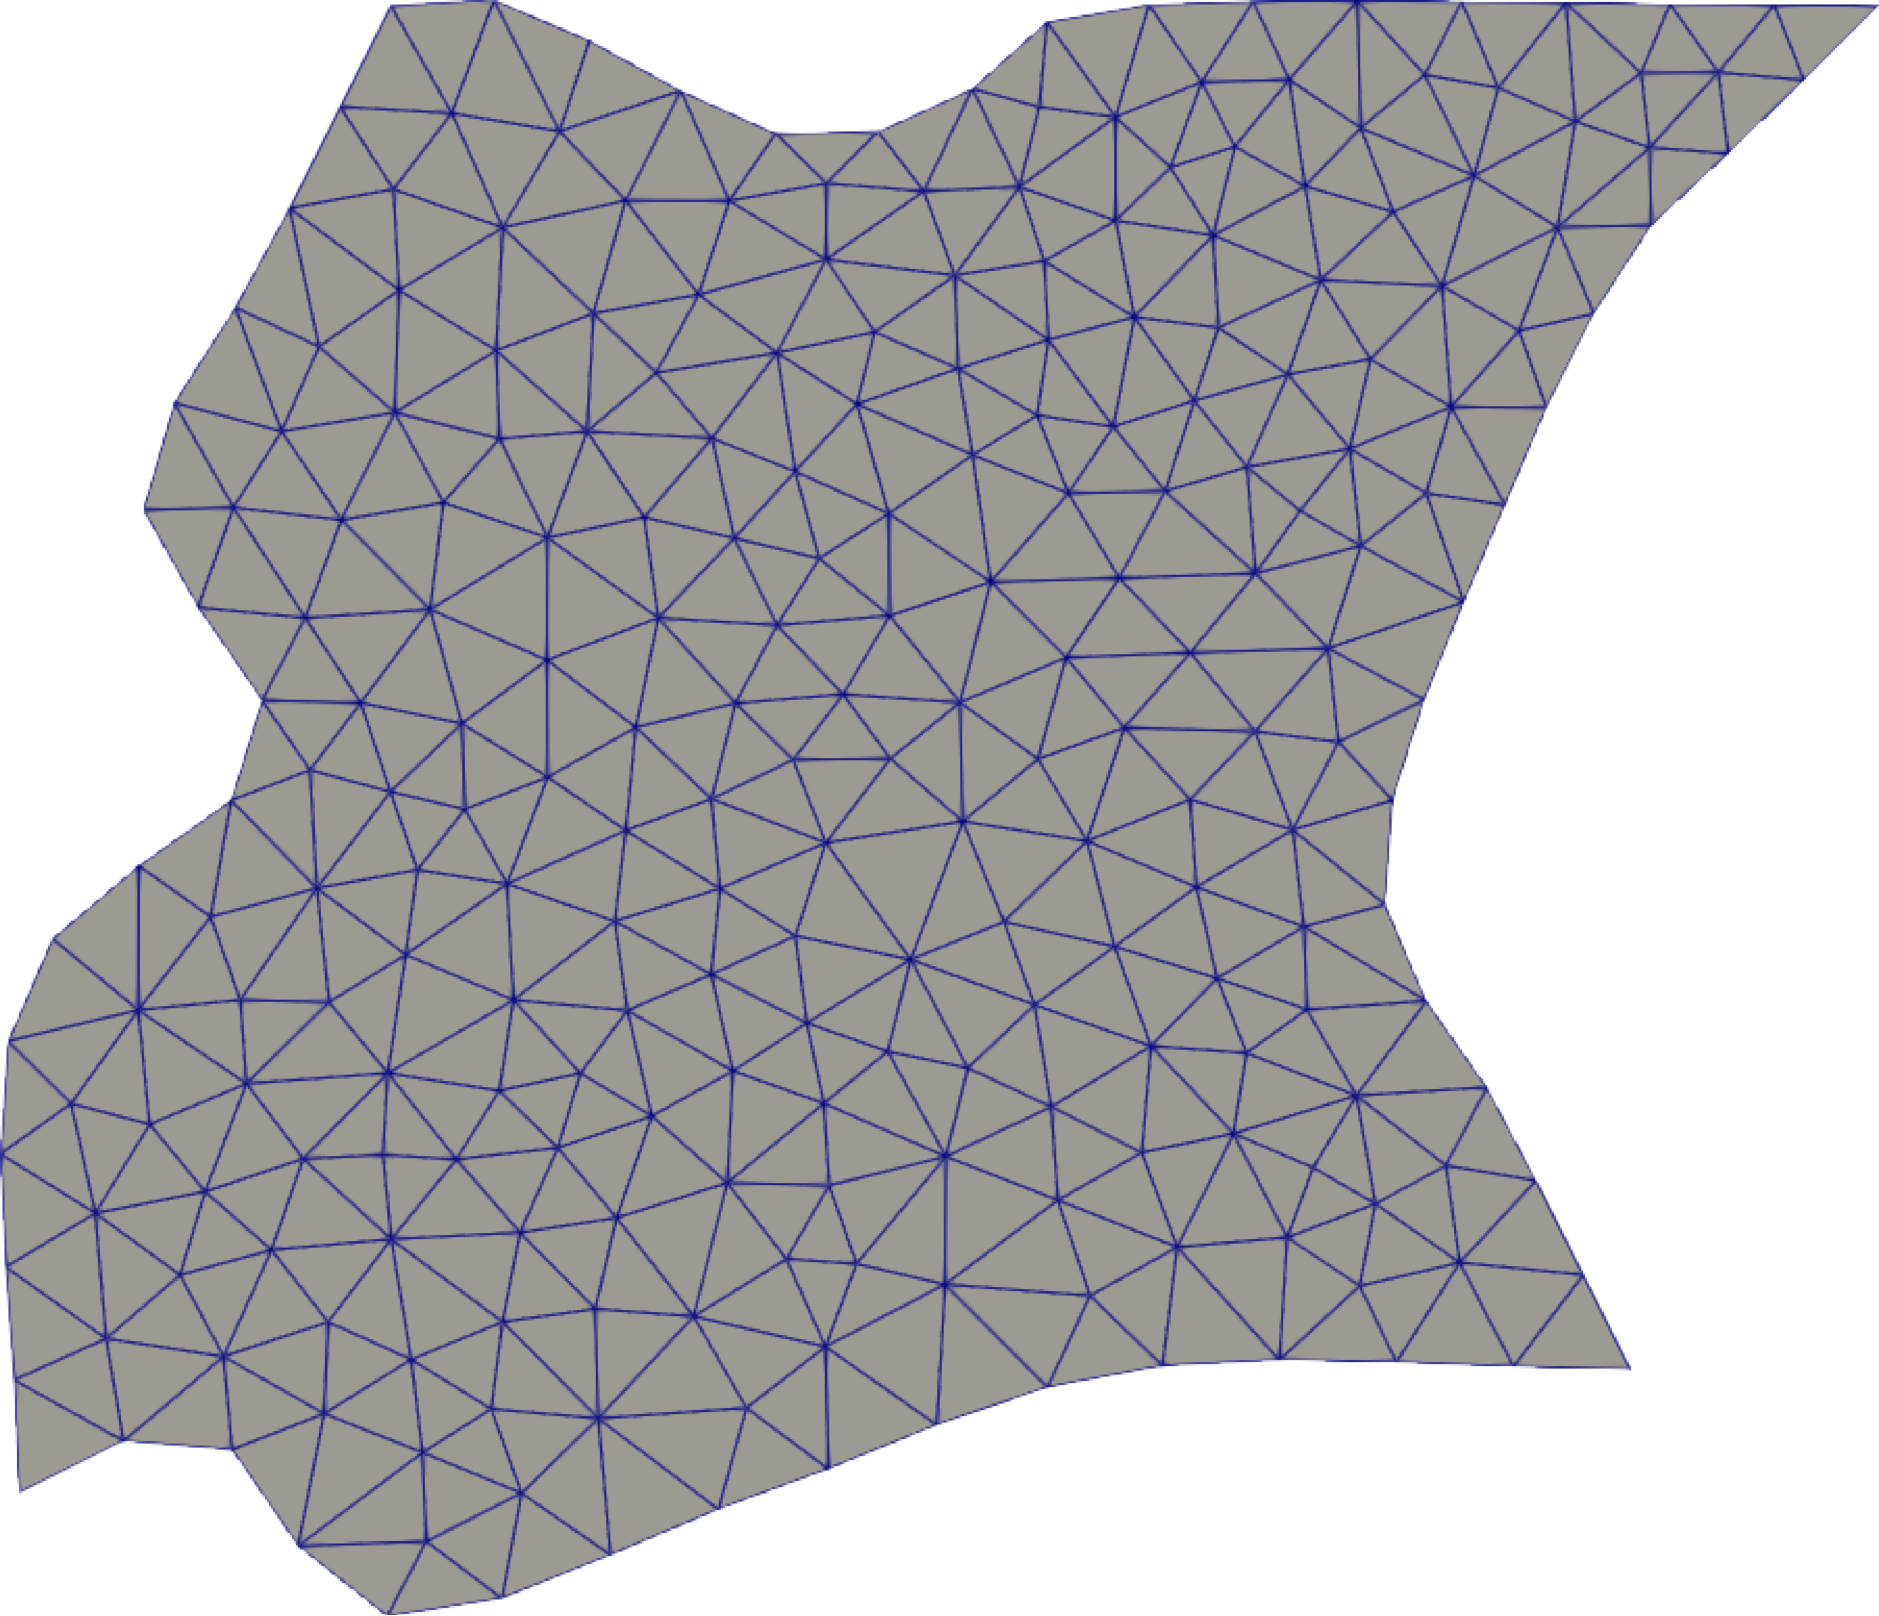
\includegraphics[scale=0.11]{images/zone4beamer.pdf}
        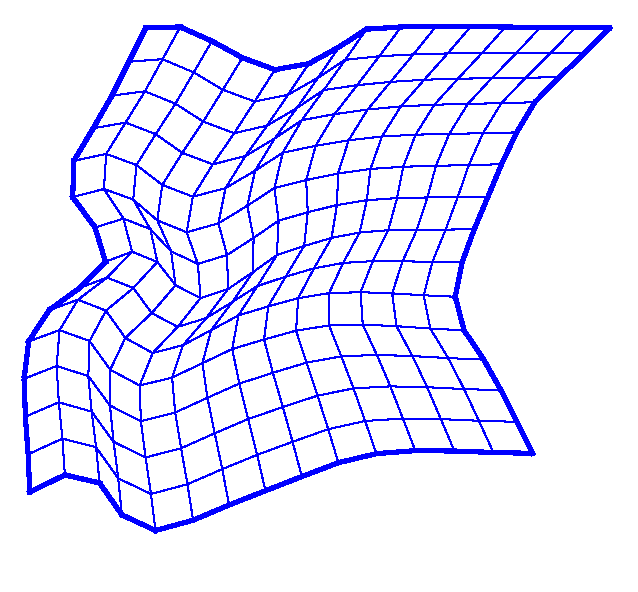
\includegraphics[scale=0.35]{images/mesh_zone4.eps}
    \end{column}
\end{columns}
\end{frame}


\begin{frame}
\frametitle{Context}
\small
\vspace{-0.2cm}
\begin{columns}
    \begin{column}{0.68\textwidth}
\textbf{The essential characteristics of high-quality quadrilateral meshes.}\vspace{0.2cm}
\begin{itemize}

\onslide<1->{
\item {\color{onera} Structured:} regularity and stability.}
\vspace{0.1cm}

\onslide<2->{
\item {\color{onera} Geometric fidelity:} cells aligned along the domain boundary, geometric conformity.}
\vspace{0.1cm}

\onslide<3->{
\item {\color{onera} High-quality elements:} cells close to squares or rectangles, minimizing the risk of degeneration during geometric transformations.}
\vspace{0.1cm}

\onslide<4->{
\item {\color{onera} Size constraint adherence:} ensures capturing local variations, overall numerical efficiency.}
\vspace{0.15cm}

\end{itemize}

\onslide<4->{
Meeting all these constraints simultaneously makes automatic generation of quadrilateral meshes challenging.}

    \end{column}

    \begin{column}{0.32\textwidth}
\centering
\only<1>{
%\vspace{-0.15cm}
    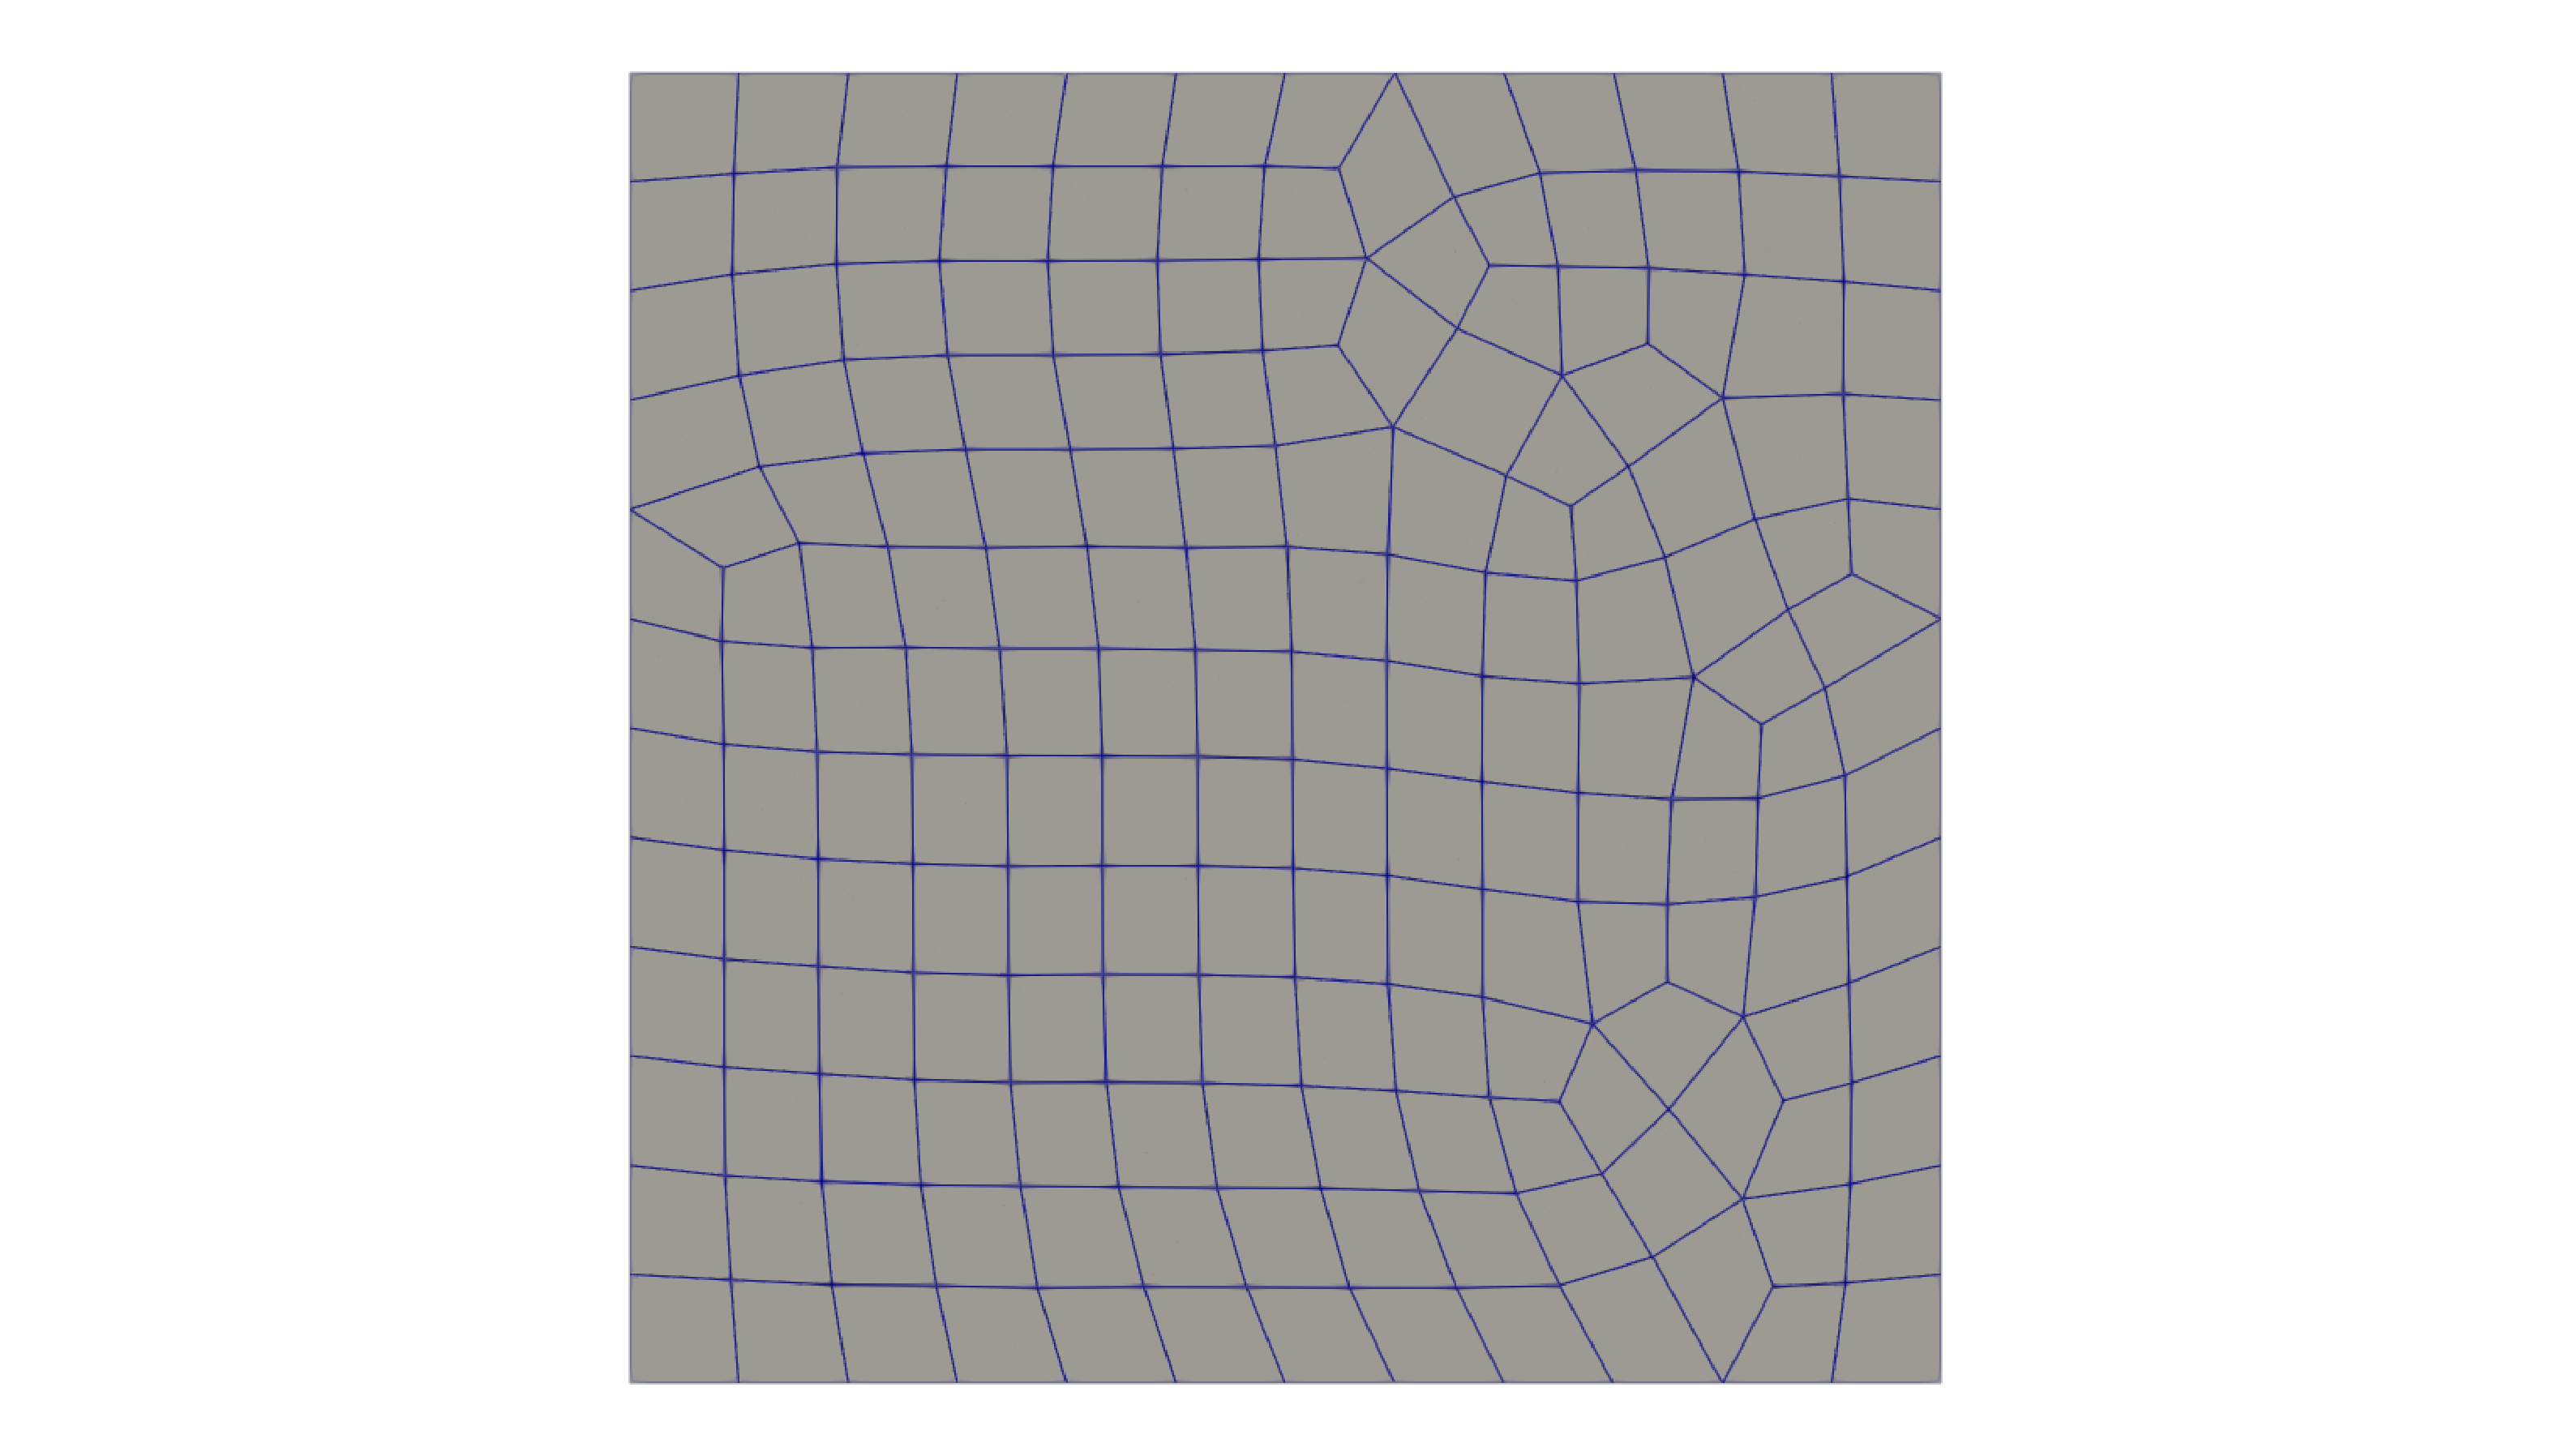
\includegraphics[scale=0.105]{images/irregularite_1.pdf}
    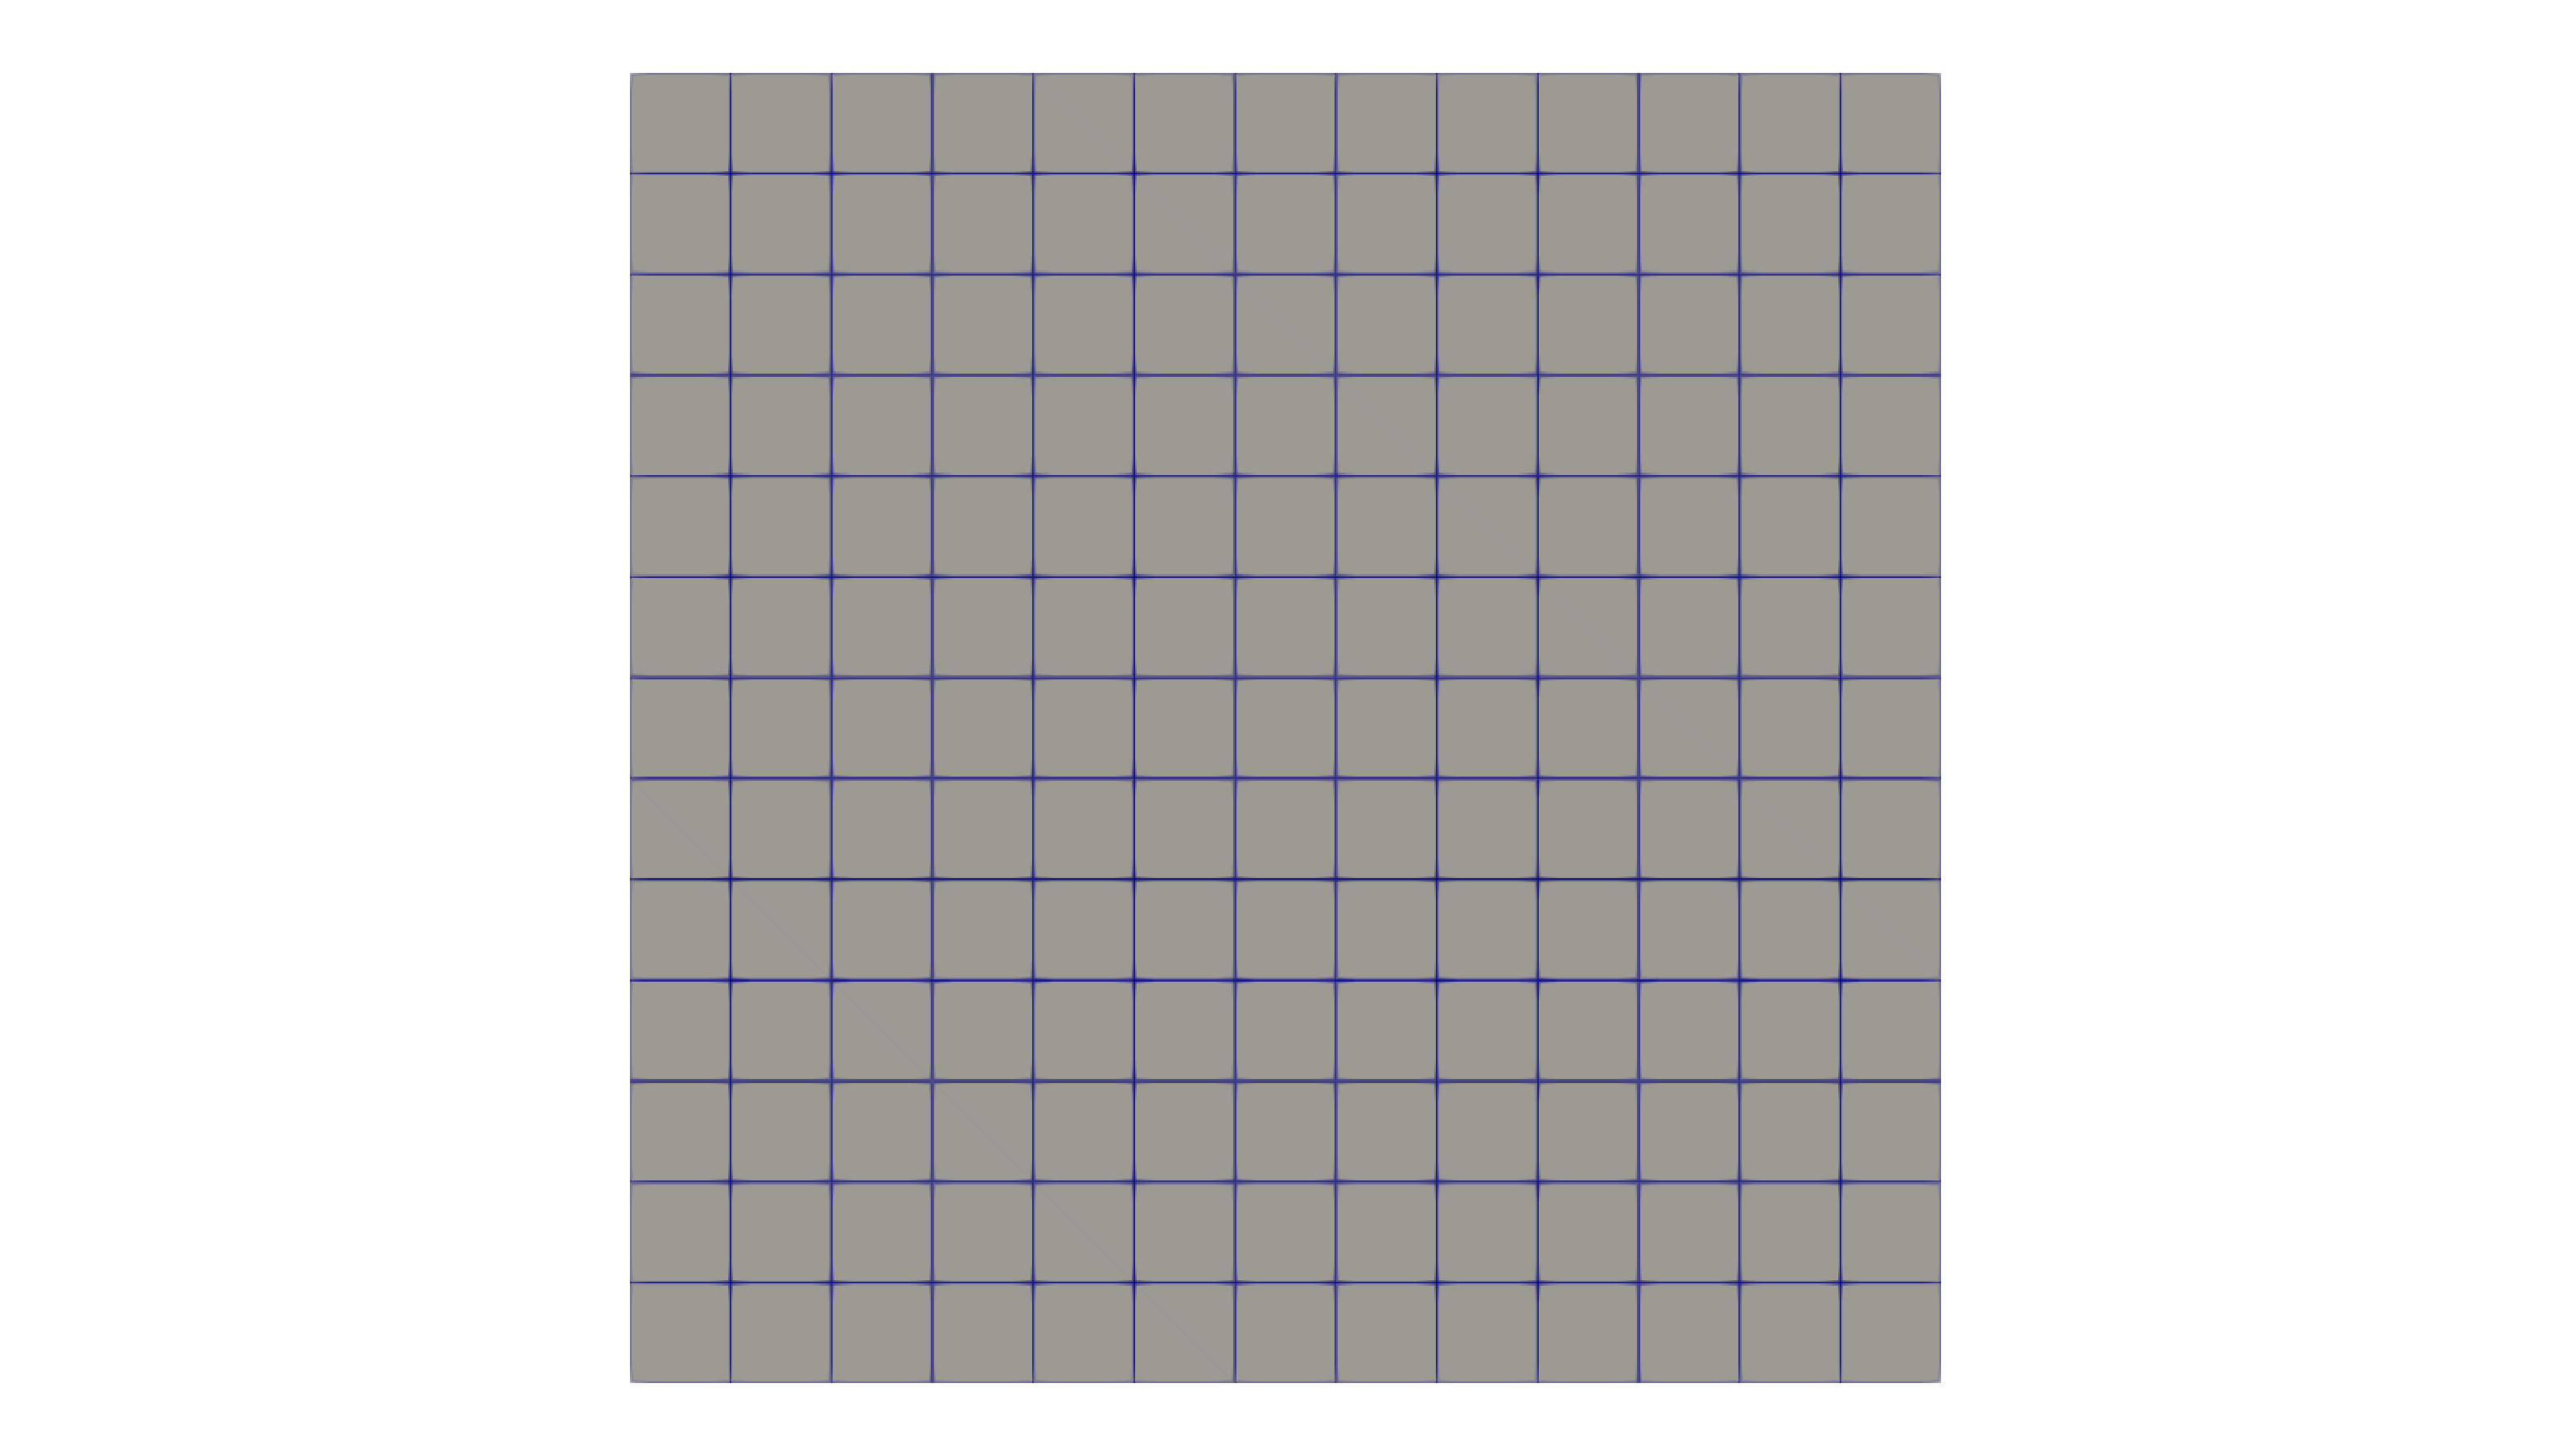
\includegraphics[scale=0.105]{images/irregularite_2.pdf}
%\vspace{0.2cm}
}
\only<2>{
\centering
%\vspace{-0.2cm}
    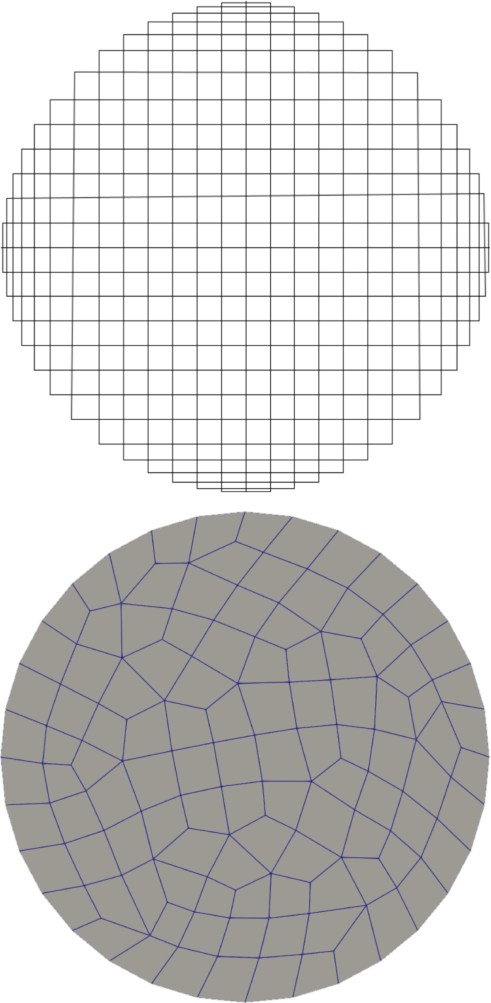
\includegraphics[scale=0.35]{images/align_bord.pdf}
\vspace{0.2cm}
}
\only<3>{
%\vspace{-0.2cm}
    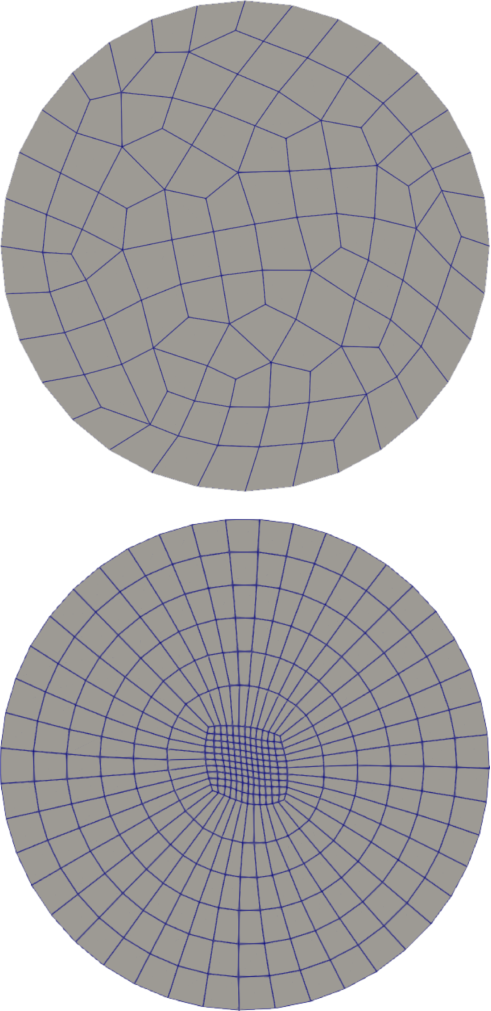
\includegraphics[scale=0.35]{images/element_quality.pdf}
\vspace{0.25cm}
}
\only<4>{
%\vspace{-0.2cm}
    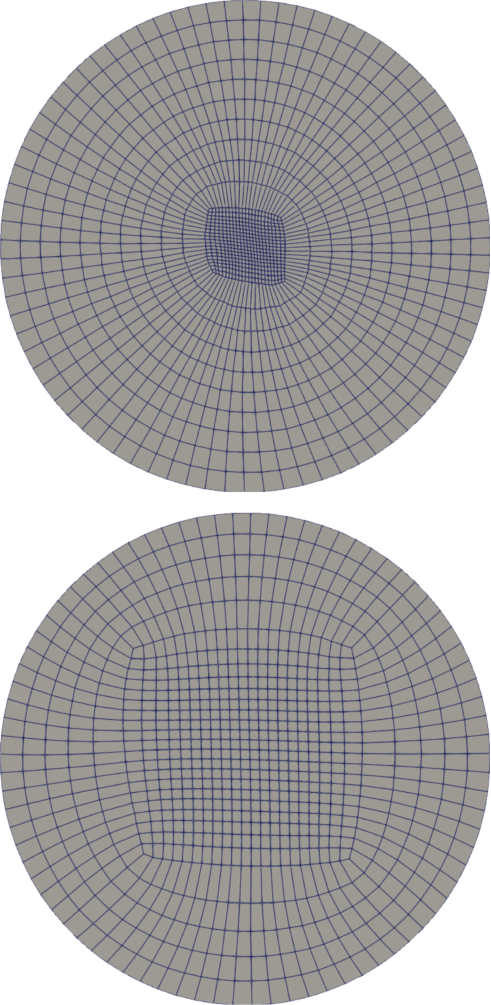
\includegraphics[scale=0.35]{images/explosion.pdf}
\vspace{0.25cm}
}
\end{column}
\end{columns}
\end{frame}



\begin{frame}
\frametitle{Context}
\small
\begin{columns}
    \begin{column}{0.6\textwidth}
        {\bf Some methods for generating "Mesh quad".}\vspace{0.2cm}
        \begin{itemize}

\onslide<1->{
            \item {\color{onera} Manual structured blocks}\\\vspace{0.1cm}}

\onslide<2->{
            \item {\color{onera} Tri-to-quad conversion:} Catmull-Clark subdivision {\color{gray} [E. Catmull, J. Clark (1978)]}, edge-flip operation {\color{onera_gray} [MeshLab, SQuad, BlossomQuad (2011)]}, unstructured quads.}\\\vspace{0.1cm}

\onslide<3->{
            \item {\color{onera} Cartesian grid methods:} domain-grid intersection {\color{onera_gray} [Schneiders (1996)]}, generate poor-quality cells along the boundary.}\\\vspace{0.1cm}

\onslide<4->{
            \item {\color{onera} Advancing front:} paving {\color{onera_gray} [D. Blacker, B. Stephenson (1991)]}, H-Morph {\color{onera_gray} [Owen et al (2000)]}.}\vspace{0.1cm}

%\onslide<5->{\item {\color{onera} Medial axis:} geometry simplification by identifying a central skeleton {\color{onera_gray} [Nackman and Srinivasan, 1989]}.}\vspace{0.1cm}

        \end{itemize}
    \end{column}

        \begin{column}{0.4\textwidth}
\centering
\only<2>{
\vspace{-0.15cm}
    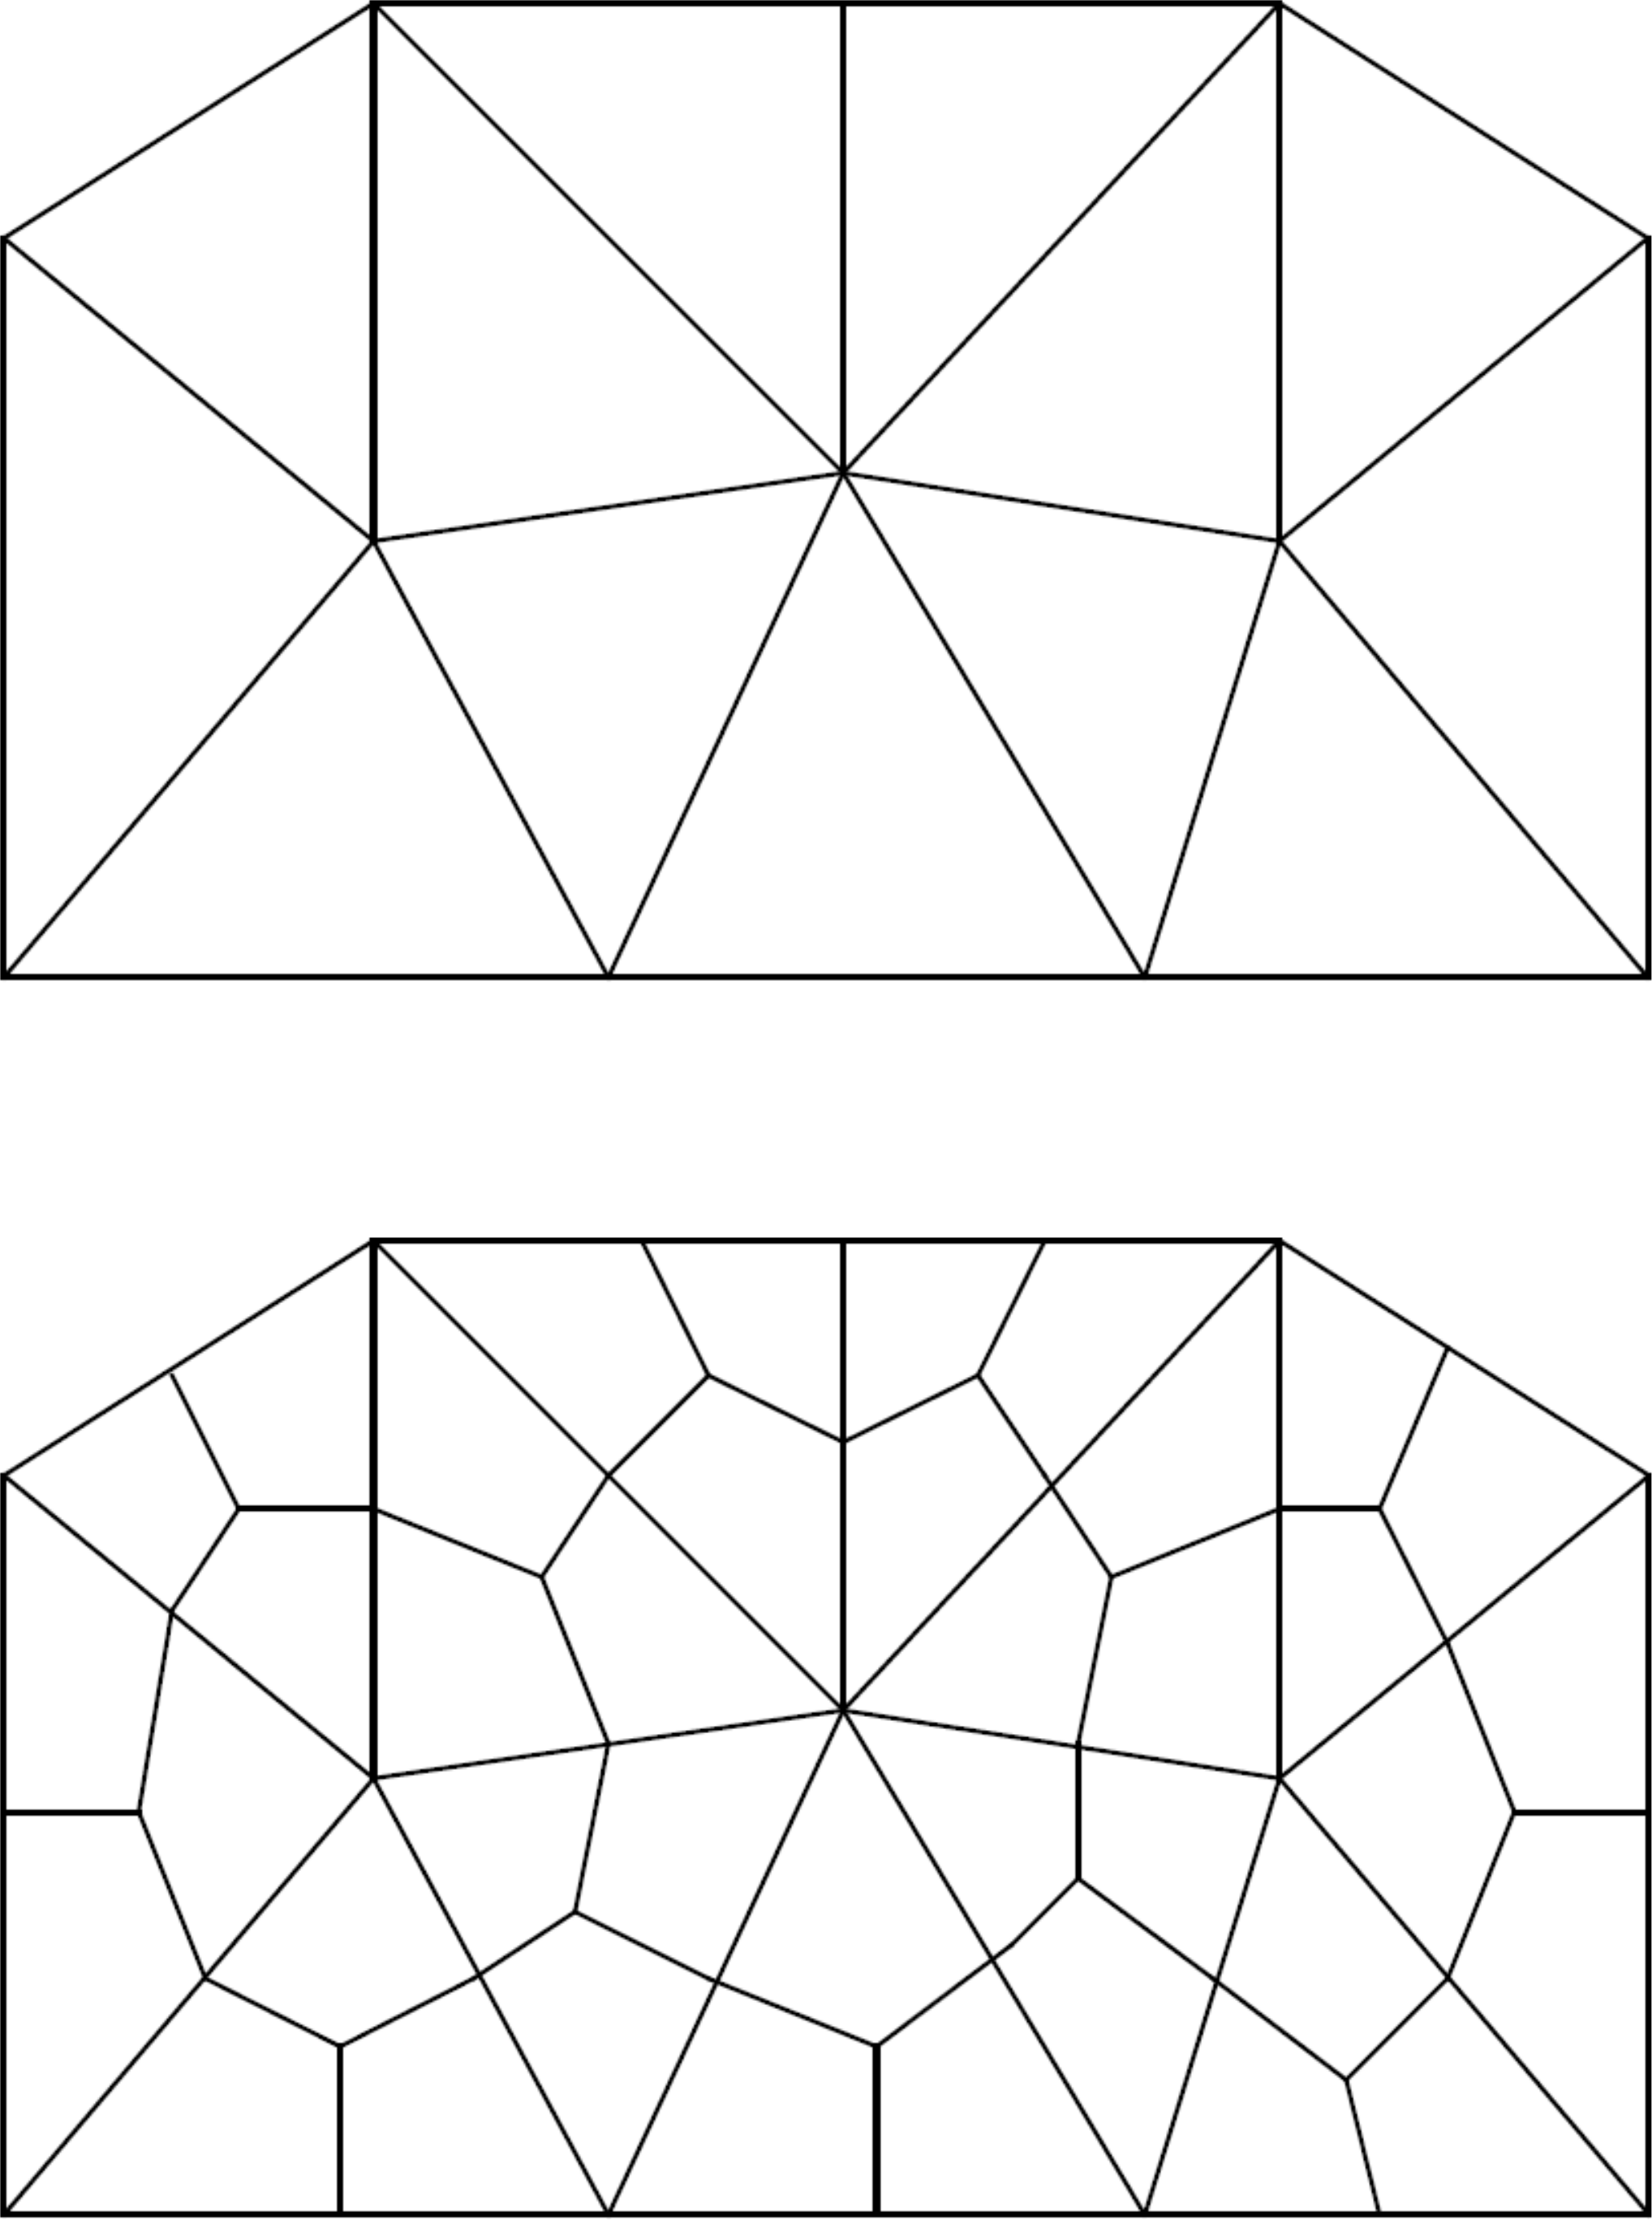
\includegraphics[scale=0.22]{images/tri_to_quad_1_beam.png}
\vspace{0.2cm}
}
\only<3>{
%\vspace{-0.2cm}
    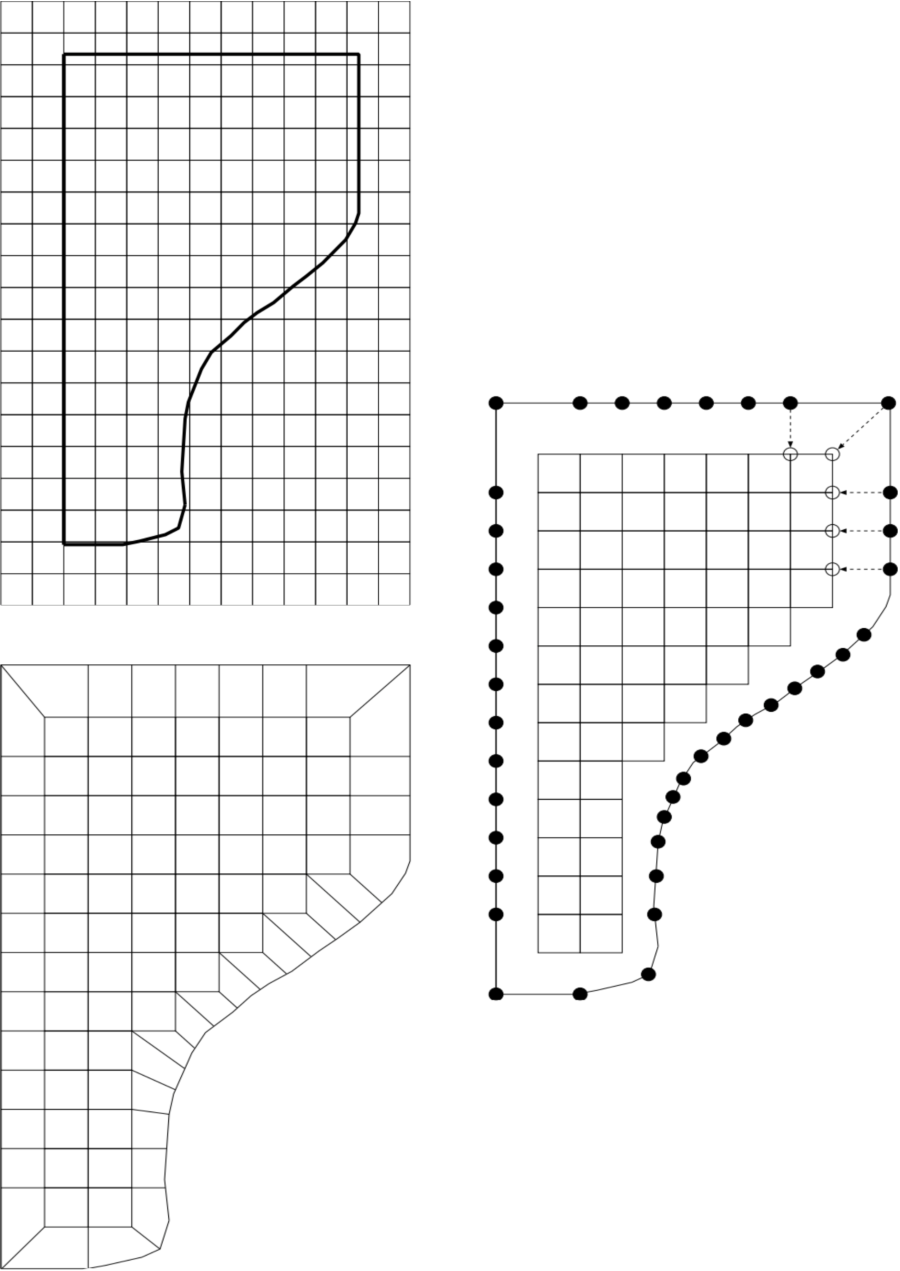
\includegraphics[scale=0.28]{images/superpo_grid_1_beam.pdf}
\vspace{0.18cm}
}
\only<4>{
\vspace{-0.2cm}
    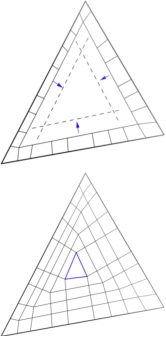
\includegraphics[scale=1]{images/front_advance_beam.pdf}
\vspace{0.15cm}
}
%\only<4>{
%\vspace{-0.2cm}
    %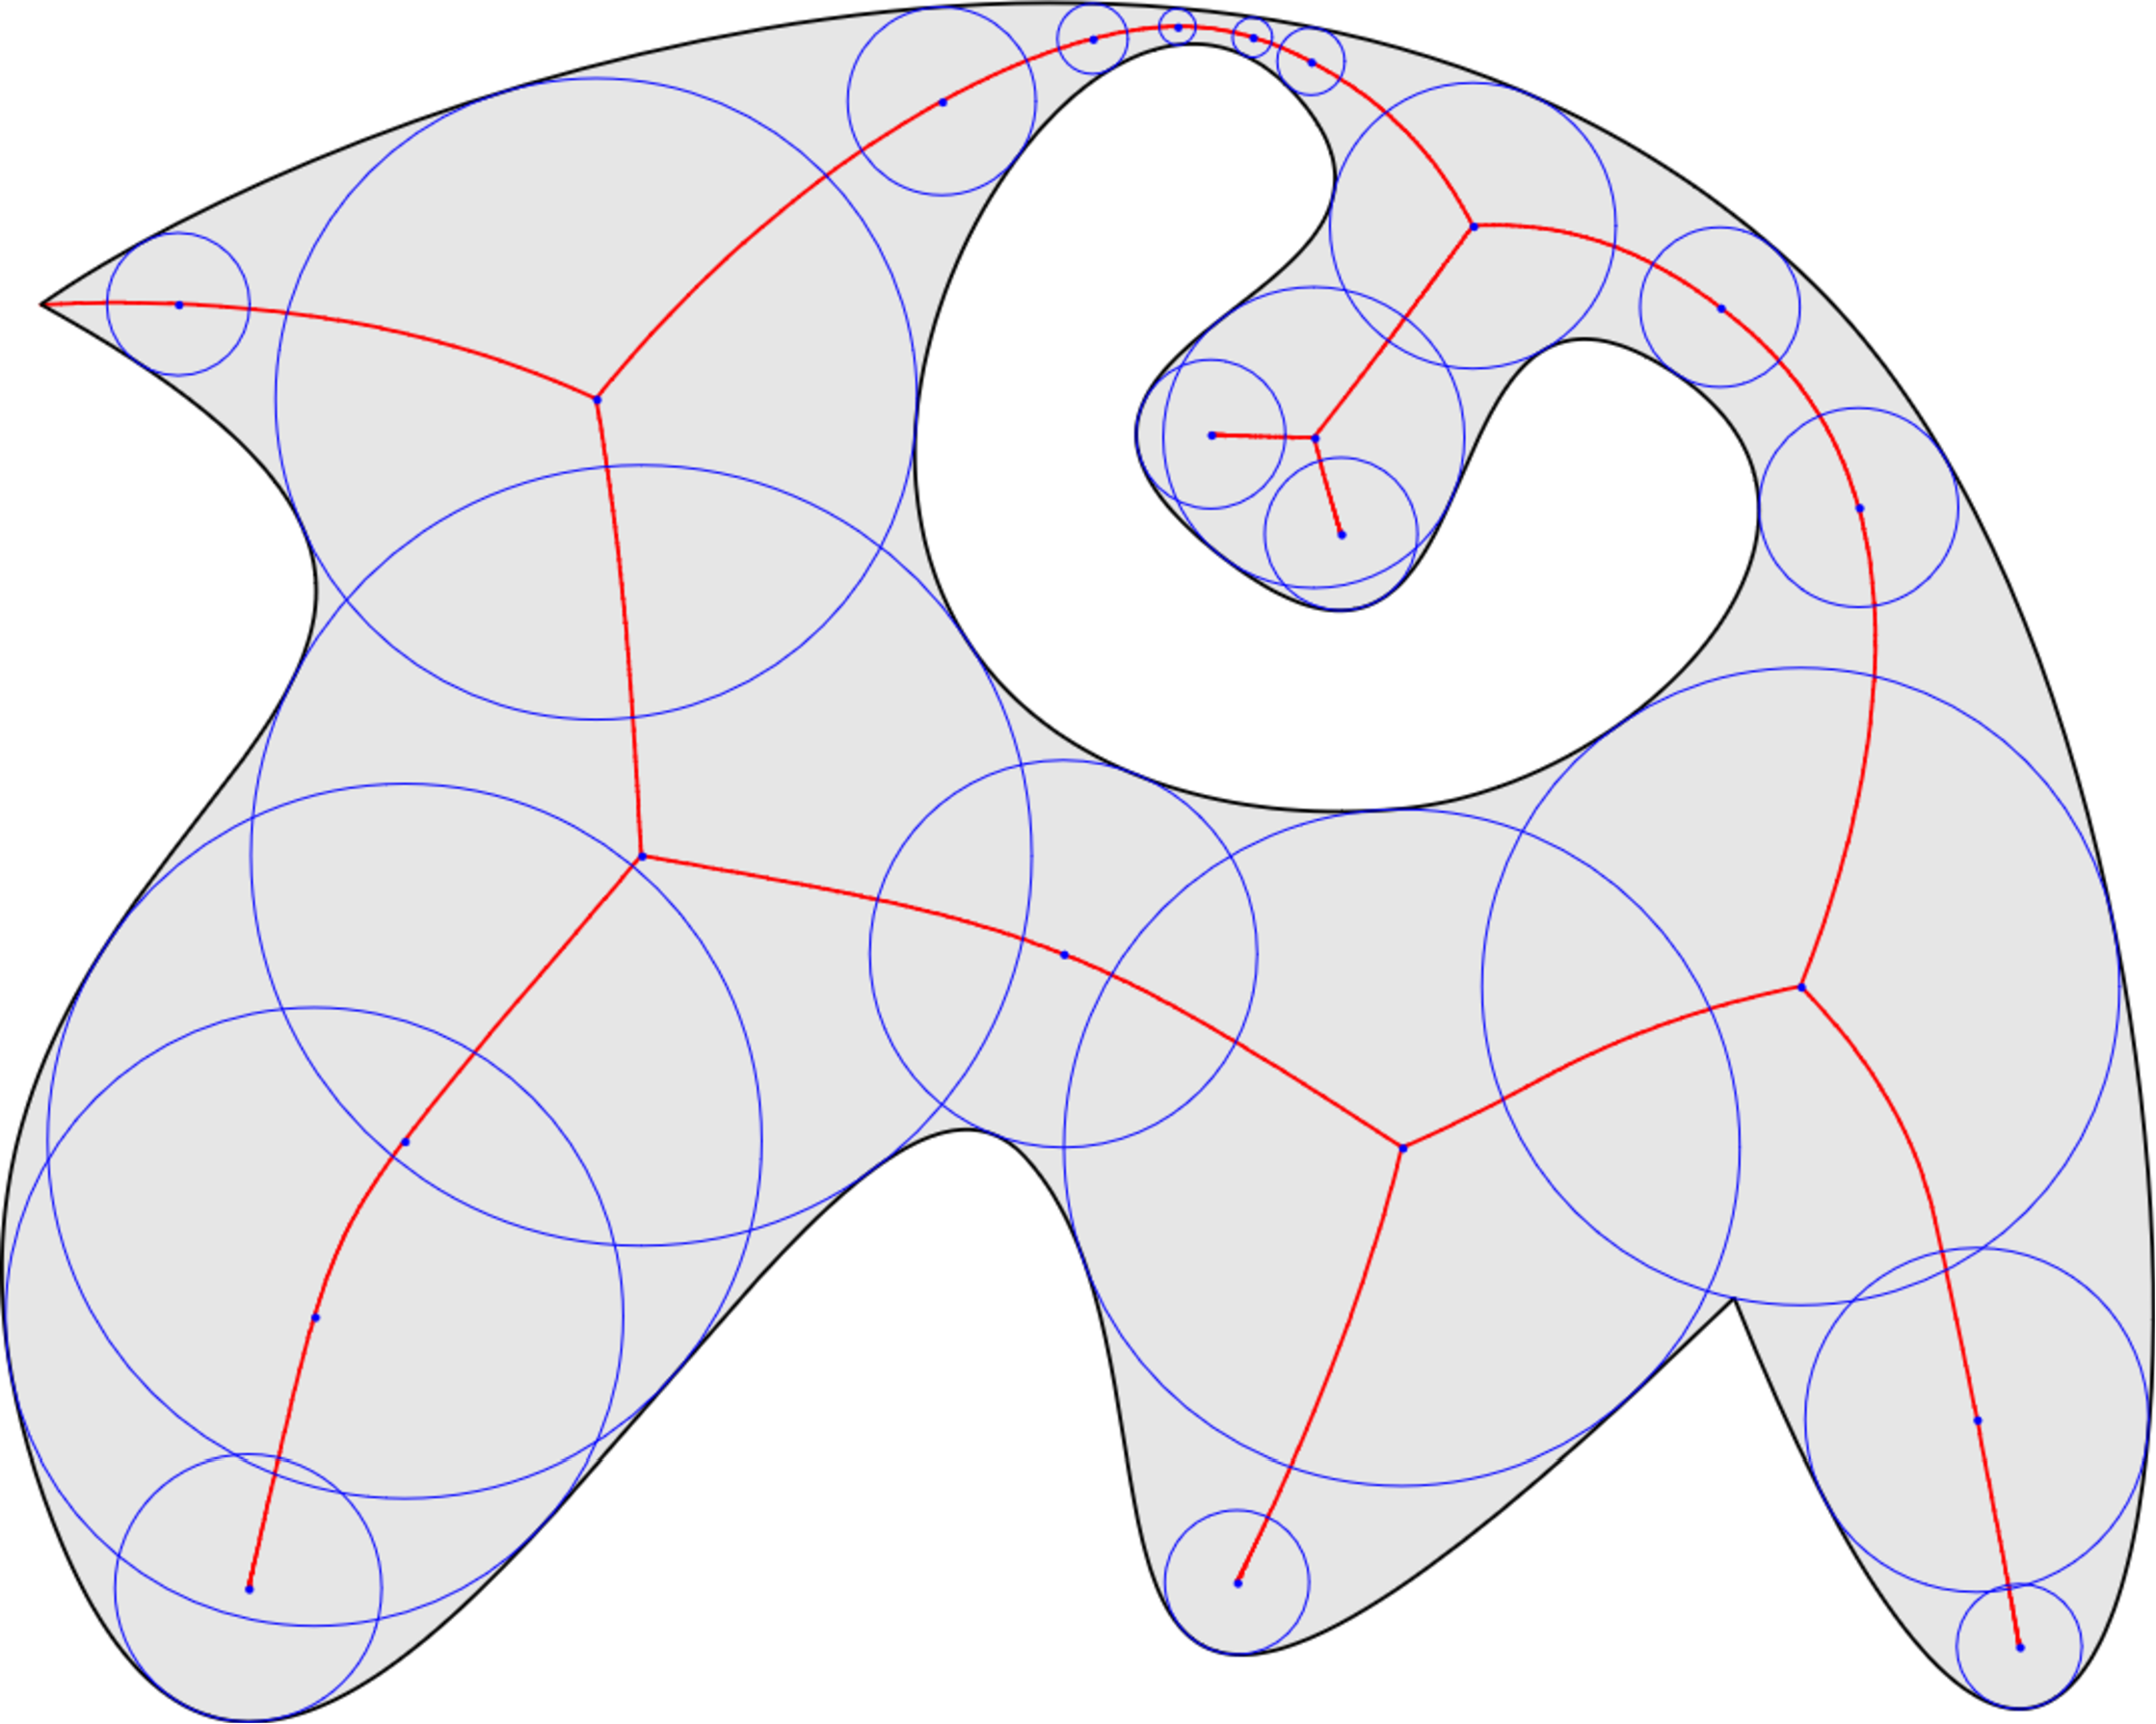
\includegraphics[scale=0.13]{images/median_axis.pdf}
%\vspace{0.15cm}
%}
\end{column}
\end{columns}
\end{frame}




\begin{frame}{A Cross-Field Based Approach}
\small
\begin{columns}

\begin{column}{0.25\textwidth}
\centering
\onslide<1->{
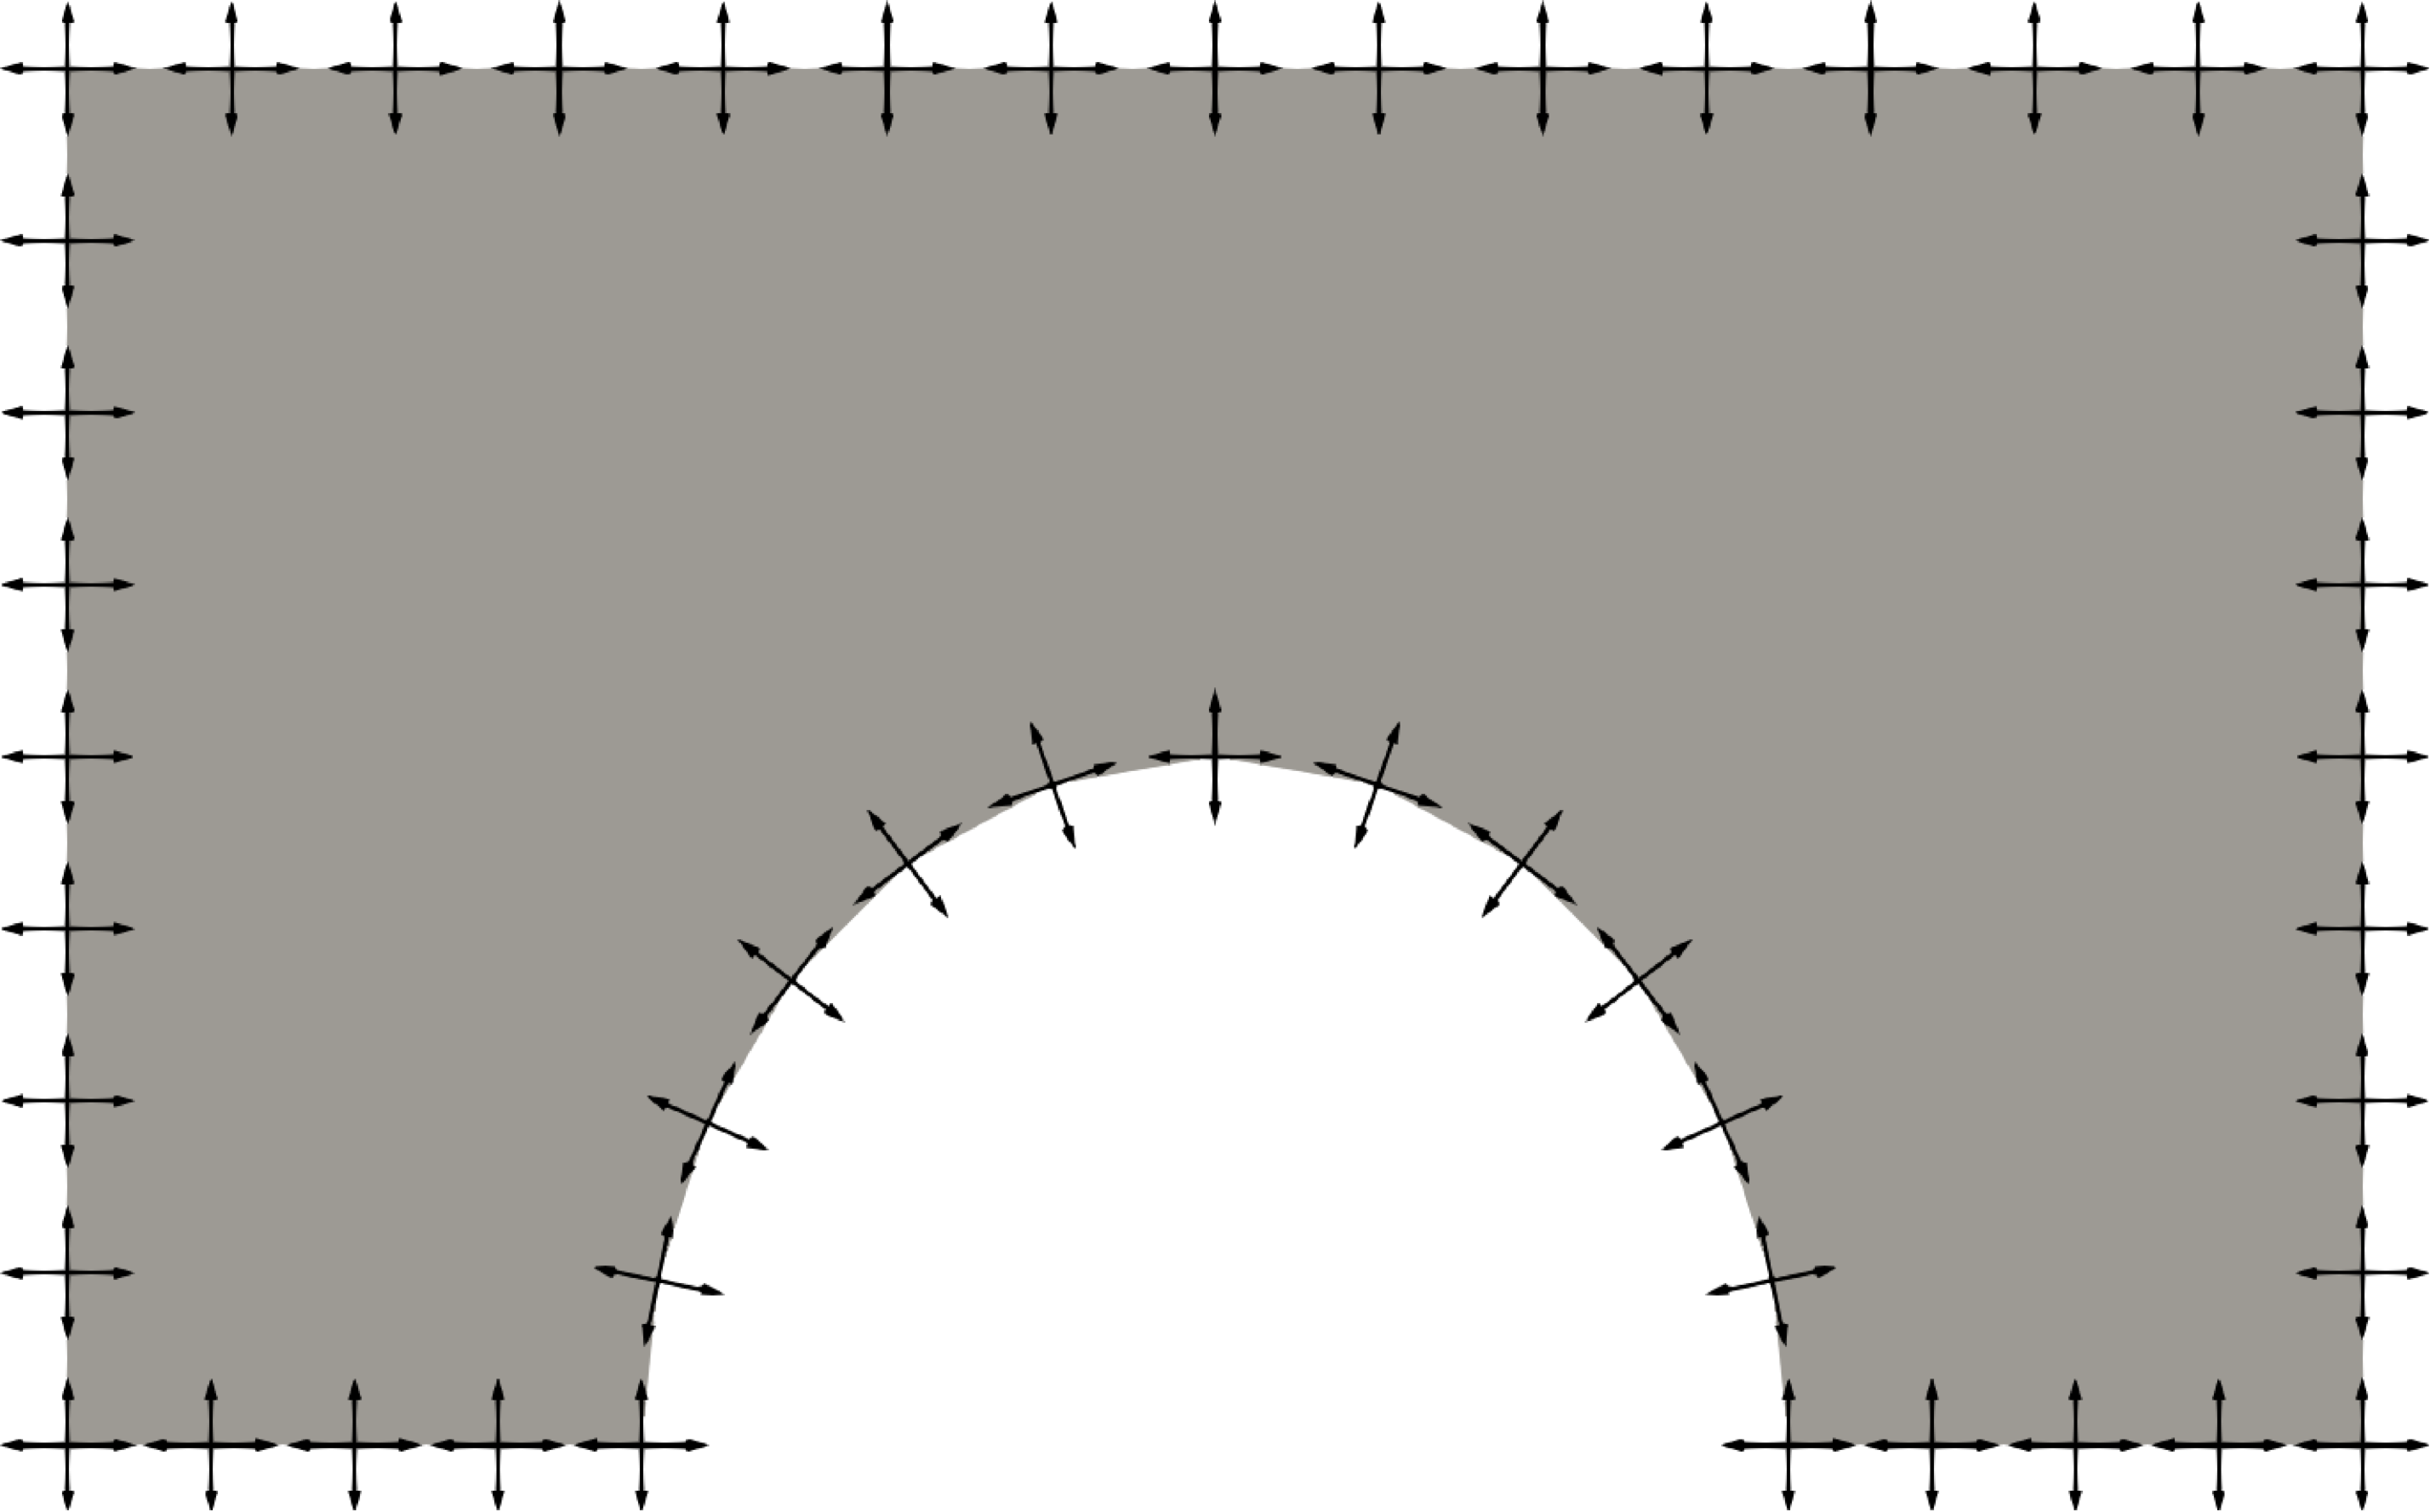
\includegraphics[scale=0.068]{images/frey_1.pdf}\hspace{0.2cm}
\footnotesize Boundary cross
}
\end{column}

\begin{column}{0.25\textwidth}
\centering
\onslide<1->{
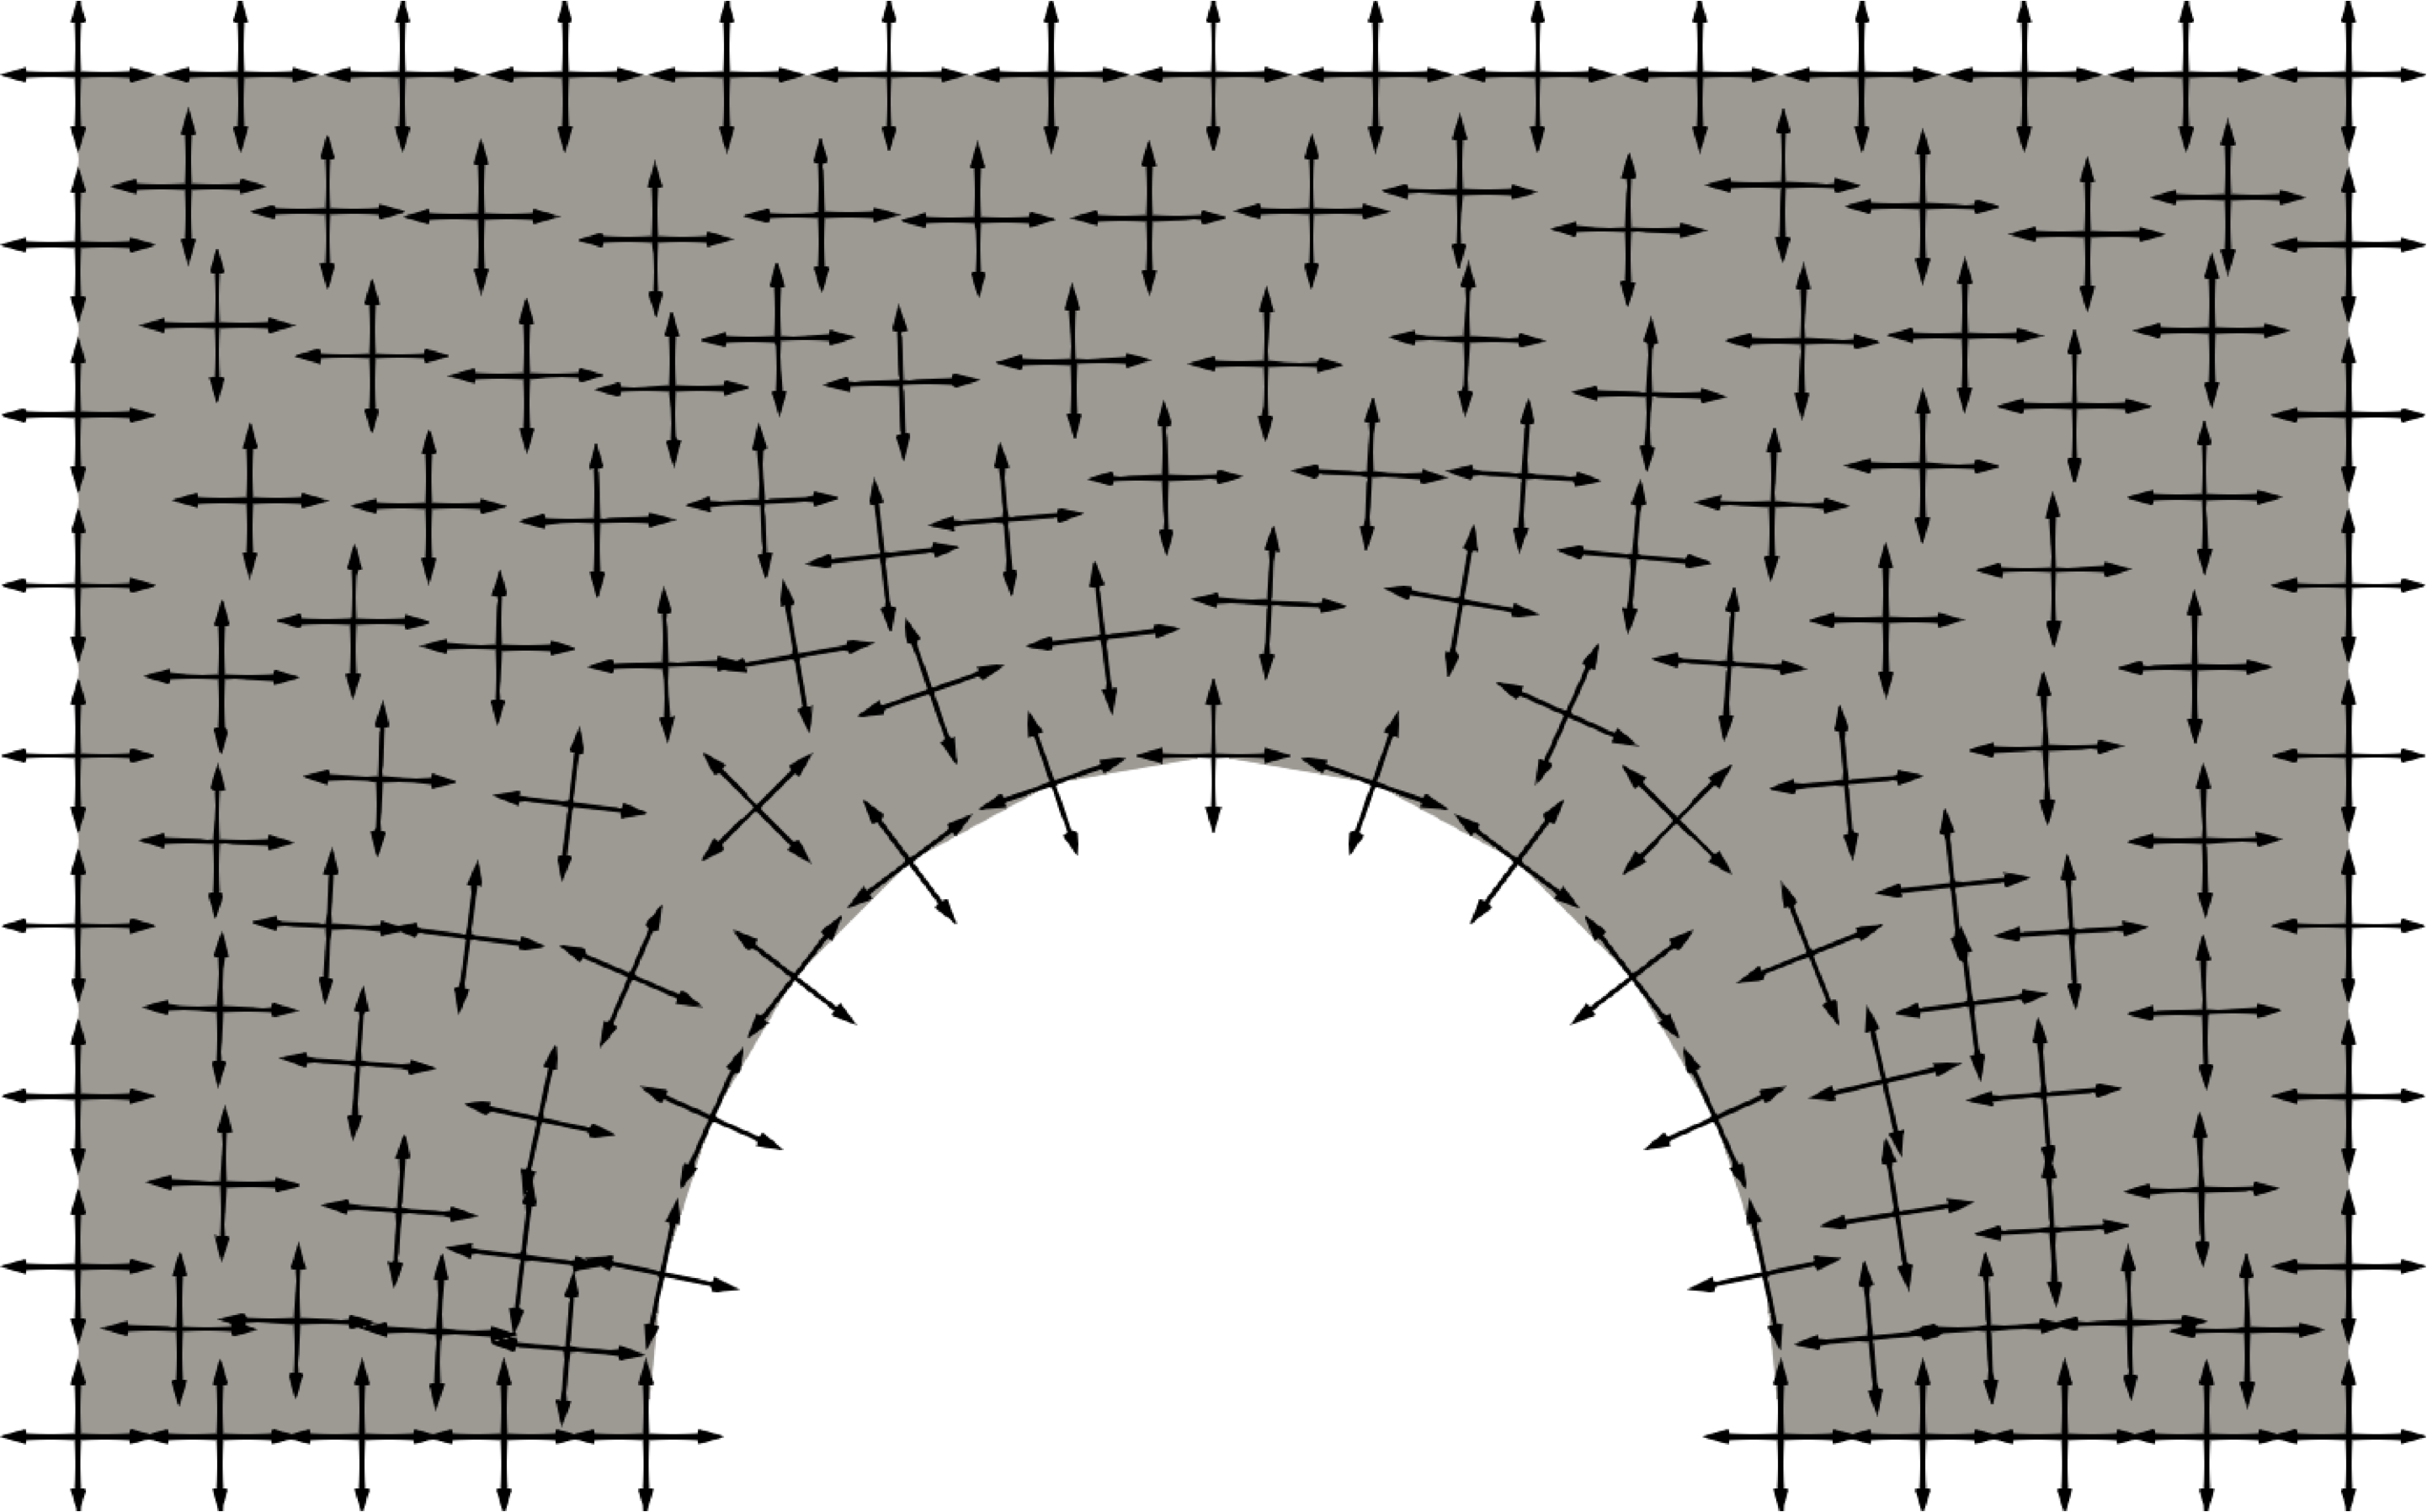
\includegraphics[scale=0.068]{images/frey_4.pdf}\hspace{0.2cm}
\footnotesize Cross-field
}
\end{column}

\begin{column}{0.25\textwidth}
\centering
\onslide<1->{
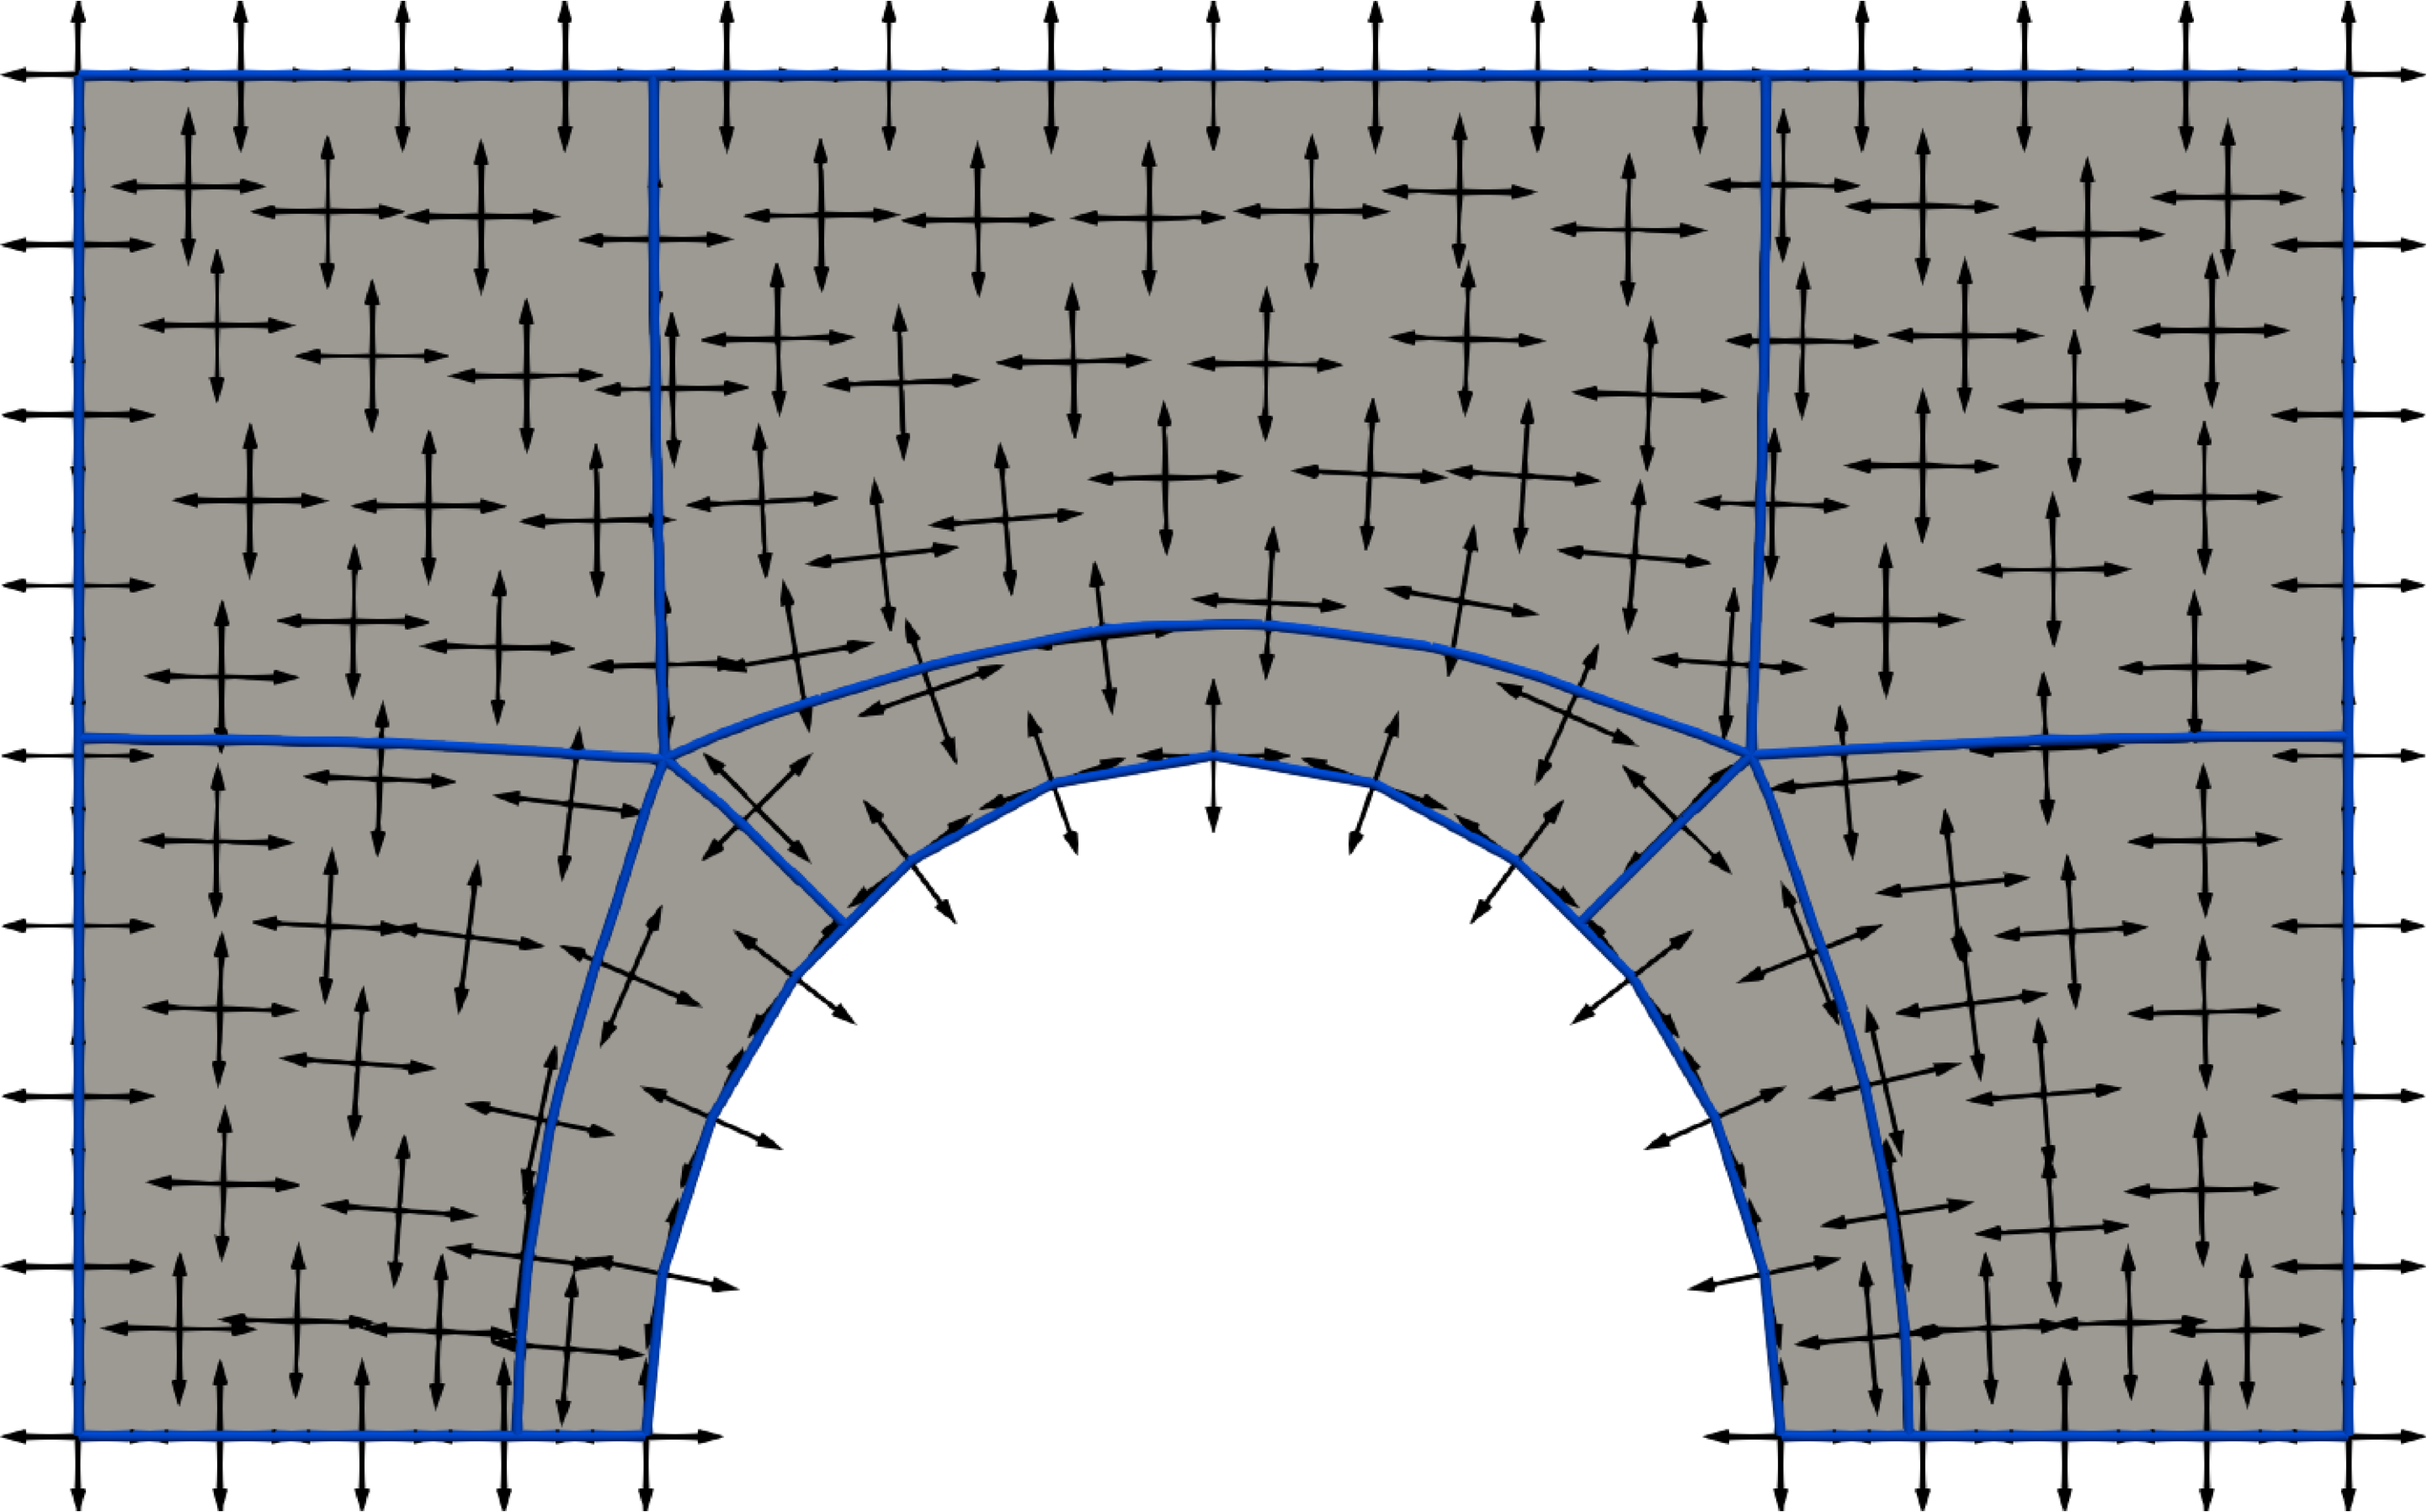
\includegraphics[scale=0.068]{images/frey_5.pdf}\hspace{0.2cm}
\footnotesize Partitioning
}
\end{column}

\begin{column}{0.25\textwidth}
\centering
\onslide<1->{
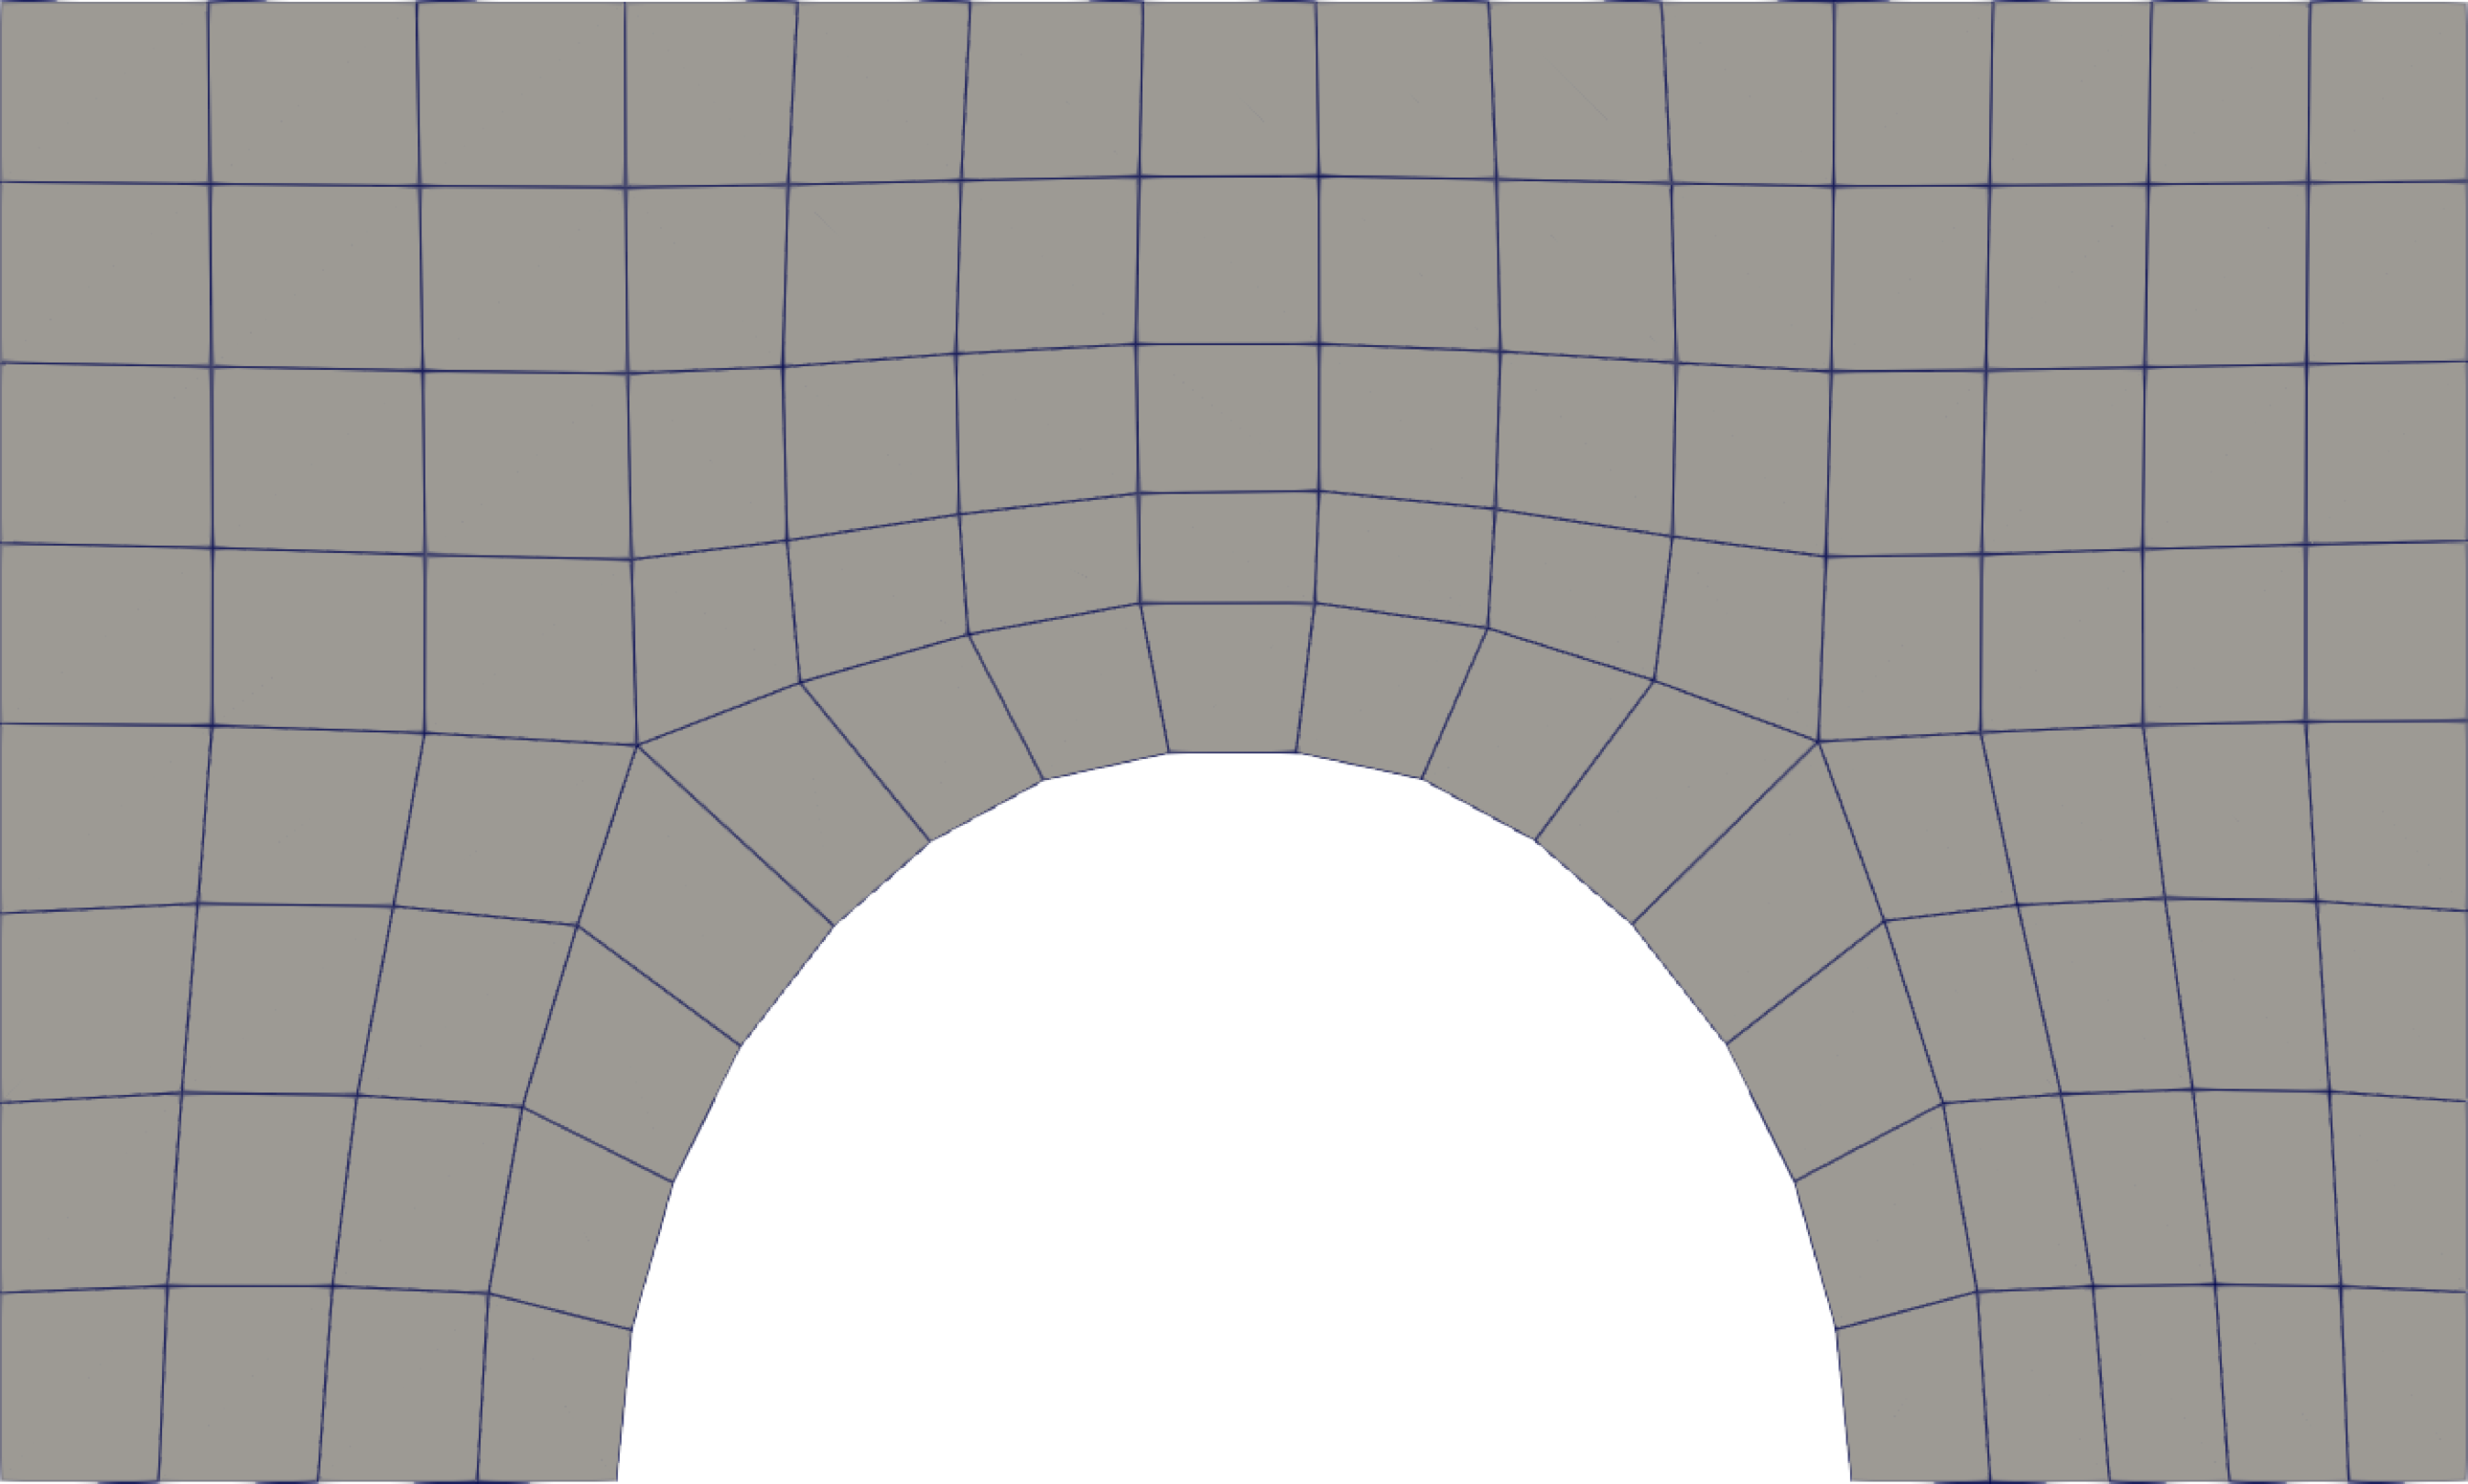
\includegraphics[scale=0.07]{images/frey_6.pdf}\vspace{0.05cm}
\footnotesize Meshing
}
\end{column}

\end{columns}

\vspace{0.4cm}

\onslide<2->{
{\bf Avantages:}

%\vspace{0.15cm}

\begin{columns}

\begin{column}{0.5\textwidth}
\begin{itemize}
\item Structured blocks: {\color{onera_gray} low storage, efficient connectivity.}\\\vspace{0.3cm}
\item Boundary adherence: {\color{onera_gray} accurate to CAD.}
%\vspace{0.4cm}
\end{itemize}
\end{column}




\begin{column}{0.5\textwidth}
\begin{itemize}
\item Element quality: {\color{onera_gray} topologically close to square, rectangle, convex.}\\\vspace{0.3cm}
\item Few irregular vertices
%\vspace{0.4cm}
\end{itemize}
\end{column}
\end{columns}
\vspace{0.35cm}
}

\end{frame}


\begin{frame}
\frametitle{A Cross-Field Based Approach}
\small
\begin{columns}
    \begin{column}{0.55\textwidth}
    \only<1>{
    {\bf Limitations of this approach:}\vspace{0.2cm}
        \begin{itemize}
            \item {\color{onera} Cross-field generation:} lack of control over singular point positions, absence of boundary singular points, non-uniformity\vspace{0.2cm}
            \item {\color{onera} Highly elongated domains:} tends to produce cross-fields with non-isolated singular points\vspace{0.2cm}
            \item {\color{onera} Method analysis:} Ginzburg-Landau approach, complex analysis, {\color{onera_gray}[Viertel et al. (2020)]}\vspace{0.2cm}
            \item {\color{onera} Surface manifolds without boundaries}
        \end{itemize}
    }

    \only<2>{
    {\bf Idea:} Implement a process to achieve quad meshes from arbitrary cross-fields\vspace{0.3cm}
        \begin{itemize}
            \item Select a cross-field with more suitable characteristics\vspace{0.3cm}
            \item Theoretical analysis of the method to understand the formation of 4-sided partitions.
        \end{itemize}
    }

    \end{column}
    \begin{column}{0.45\textwidth}
        \centering
        \vspace{-0.15cm}
        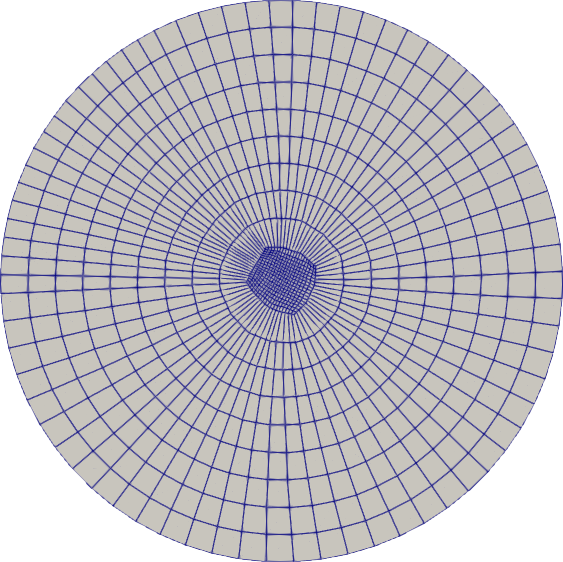
\includegraphics[scale=0.12]{images/new_cercle.png}
        \hspace{0.6cm}
        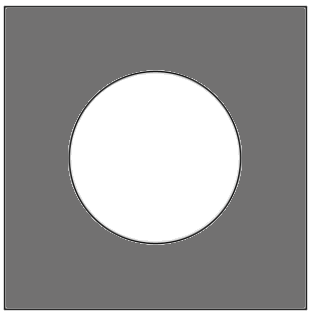
\includegraphics[scale=0.28]{images/carreTrou.png}
        \\\vspace{0.2cm}
        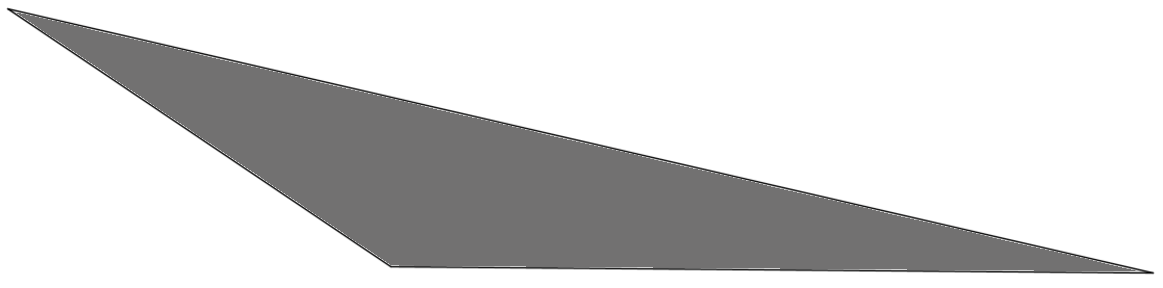
\includegraphics[scale=0.18]{images/triangle_etire.png}
        \hspace{0.2cm}
        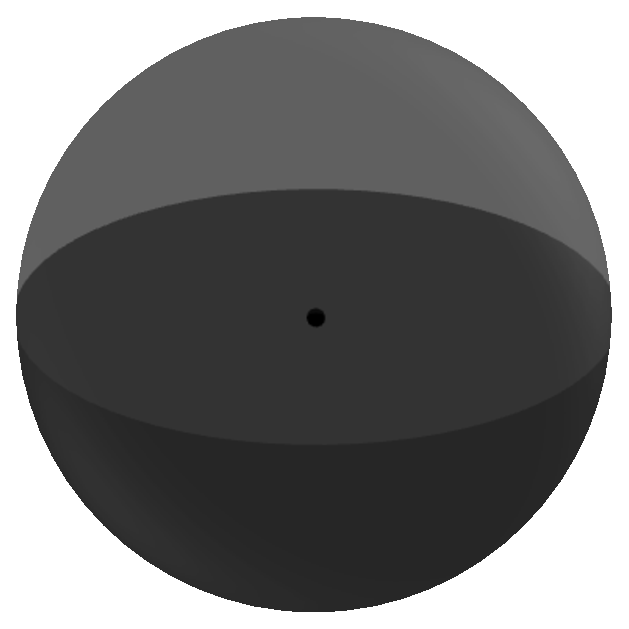
\includegraphics[scale=0.23]{images/sphere.eps}
        \vspace{0.3cm}
    \end{column}
\end{columns}
\end{frame}


\begin{frame}{Outline}
    %\tableofcontents
    \vspace{-0.4cm}
    \begin{enumerate}
        \item \color{onera} Context and Objectives \\\vspace{0.26cm}
        \item Formalizing the Partitioning Process %{\color{onera_gray}(new perspective, field alignment on the boundary, ...)}
        \vspace{0.26cm}
        \begin{itemize}
            \item Handling Arbitrary Cross-Fields\\\vspace{0.18cm}
            \item Alignment Process\\\vspace{0.18cm}
            \item Non-Simply Connected Domains\\\vspace{0.18cm}
            %\item Discussions (some theoretical results)\\\vspace{0.18cm}
            %\item Examples%\\\vspace{0.2cm}
        \end{itemize}
        %\item Handling Boundary Singularities {\color{onera_gray}(considering boundary conditions, ...)}\\\vspace{0.5cm}
        %\item Handling Arbitrary Cross-Fields {\color{onera_gray}(domains with holes, multi-material, ...)}\\\vspace{0.34cm}
        \item Discretization and Extension to Non-Planar Surface Manifolds %{\color{onera_gray}(considering curvature, generalization, ...)}\\
        \vspace{0.26cm}
        \begin{itemize}
            \item Partitioning Process\\\vspace{0.18cm}
            \item Convergence Analysis\\\vspace{0.18cm}
            %\item Examples%\\\vspace{0.2cm}
        \end{itemize}
        \item Conclusion and Perspectives
    \end{enumerate}
\end{frame}


\begin{frame}{Handling Arbitrary Cross-Fields}
\small
A {\color{onera}cross} is an element of the quotient set $\mathbb{S}^1/\mathcal{Q}\cup\{0\}$ {\color{onera_gray}(unit circle, set of 4 vectors)}.\\\vspace{0.2cm}
A {\color{onera}cross-field} is a mapping $\bar{u}:p\in\Omega\rightarrow \bar{u}(p)\in S^1/\mathcal{Q}\cup\{0\}$.\\\vspace{0.2cm}

\begin{onerablock}[drop fuzzy shadow]{\small Definition}
\small
$\bar{u}$ is an \emph{almost-$\mathcal{C}^1$} cross-field if $\bar{u}$ is of class $\mathcal{C}^1$ at every point except at a finite number of points {\color{onera_gray}(the singular points)}.
\end{onerablock}

{\bf\underline{Example:}} {\color{onera_gray} cross-field from an eigenmode of the Laplacian on the half-disk. Tangent and gradient of the isolines. Singular points and extrema. Quarter angle of the crosses. Partitioning. Tool.}

    \begin{columns}
        \begin{column}{0.33\textwidth}
        \centering
\onslide<2->{
        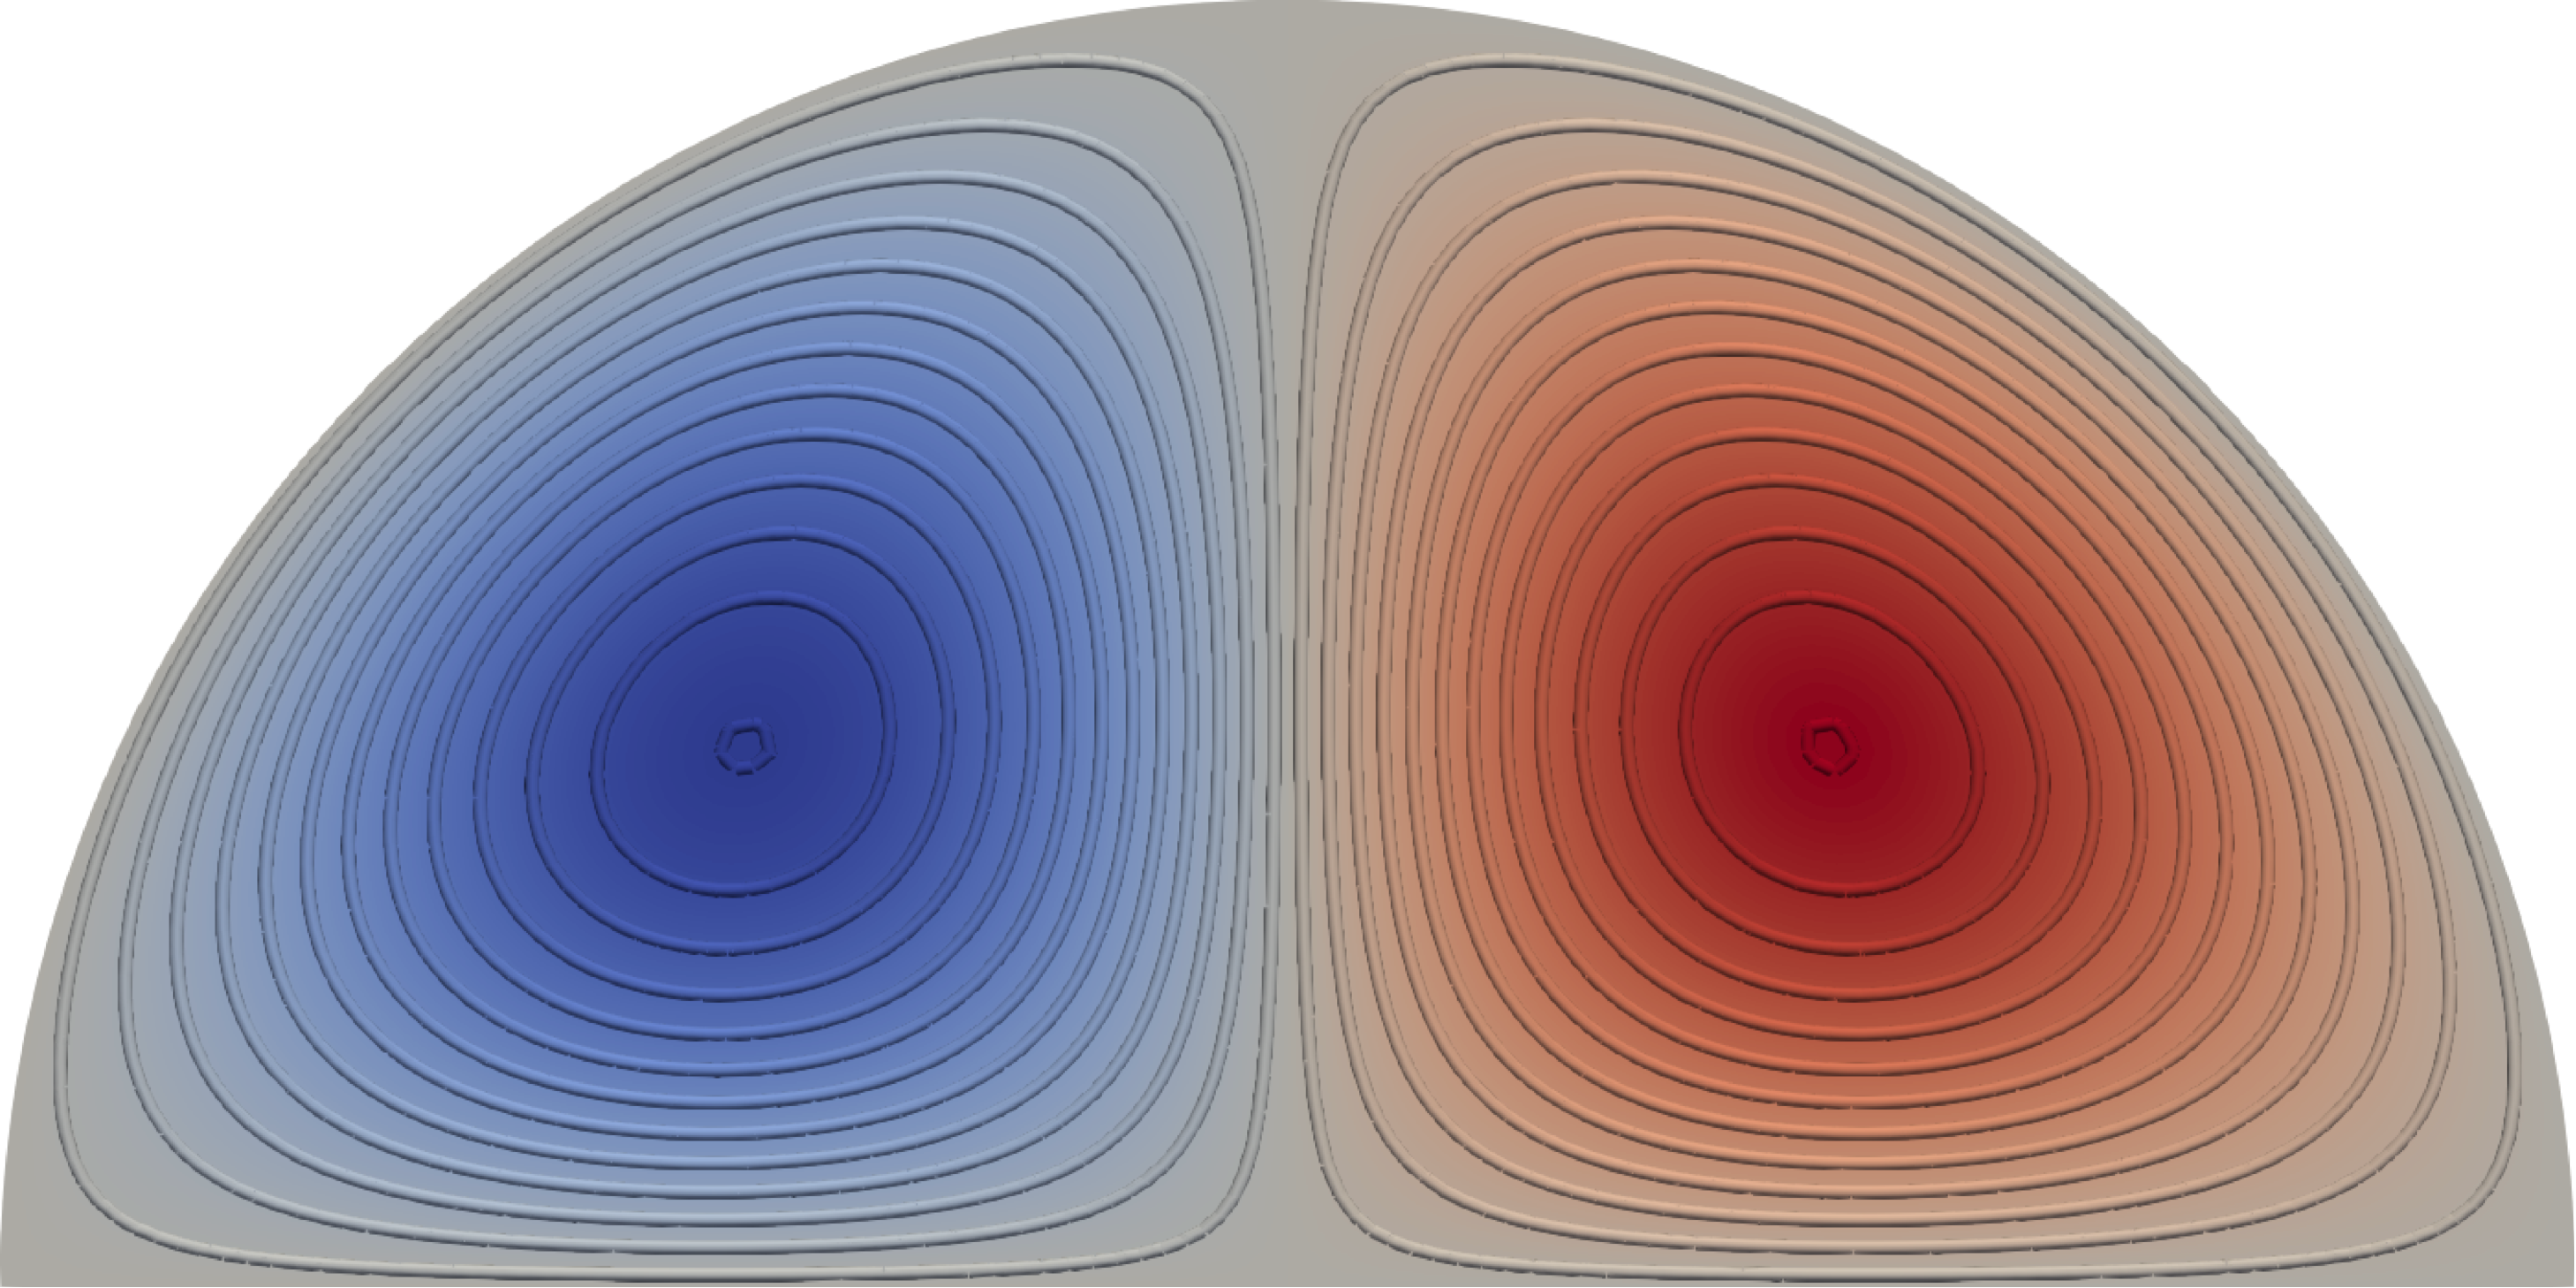
\includegraphics[scale=0.092]{images/mode_prop_new.pdf} \hspace{0.2cm}
        %\footnotesize Eigenmode of the Laplacian on the half-disk
        }
        \end{column}
        \begin{column}{0.33\textwidth}
        \centering
\onslide<2->{
        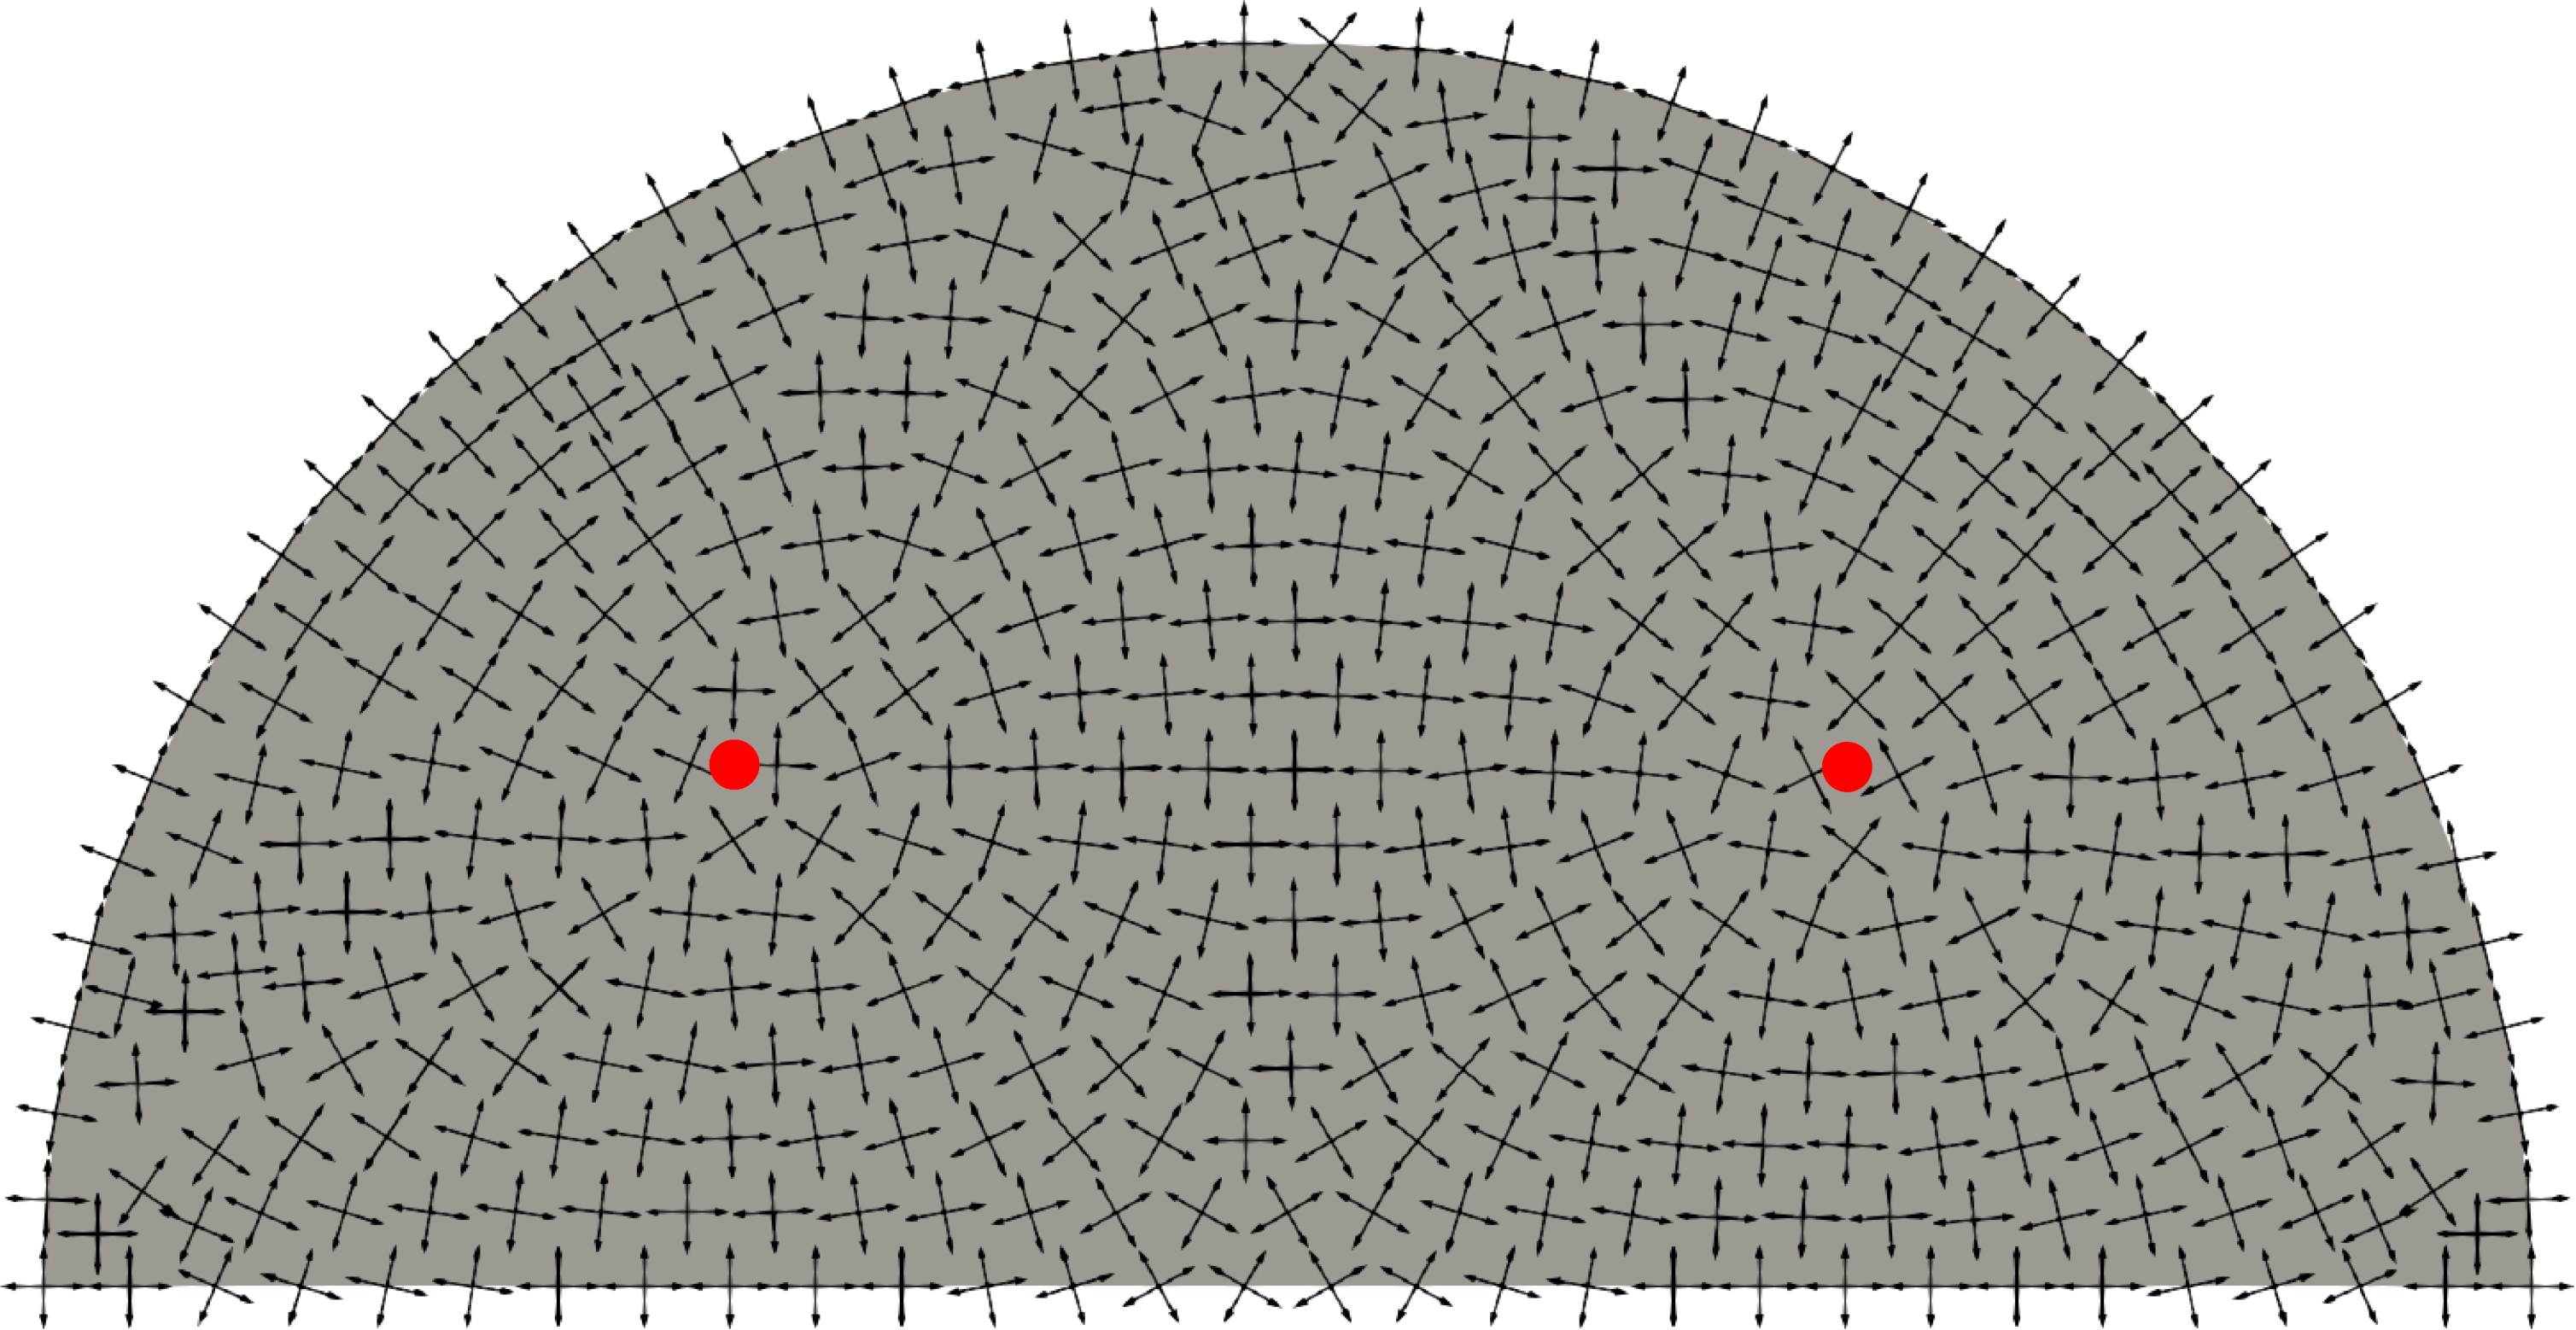
\includegraphics[scale=0.092]{images/tang_grad.pdf} \hspace{0.2cm}
        %\footnotesize Tangents to the level lines
        }
        \end{column}
        \begin{column}{0.33\textwidth}
        \centering
\only<3>{
        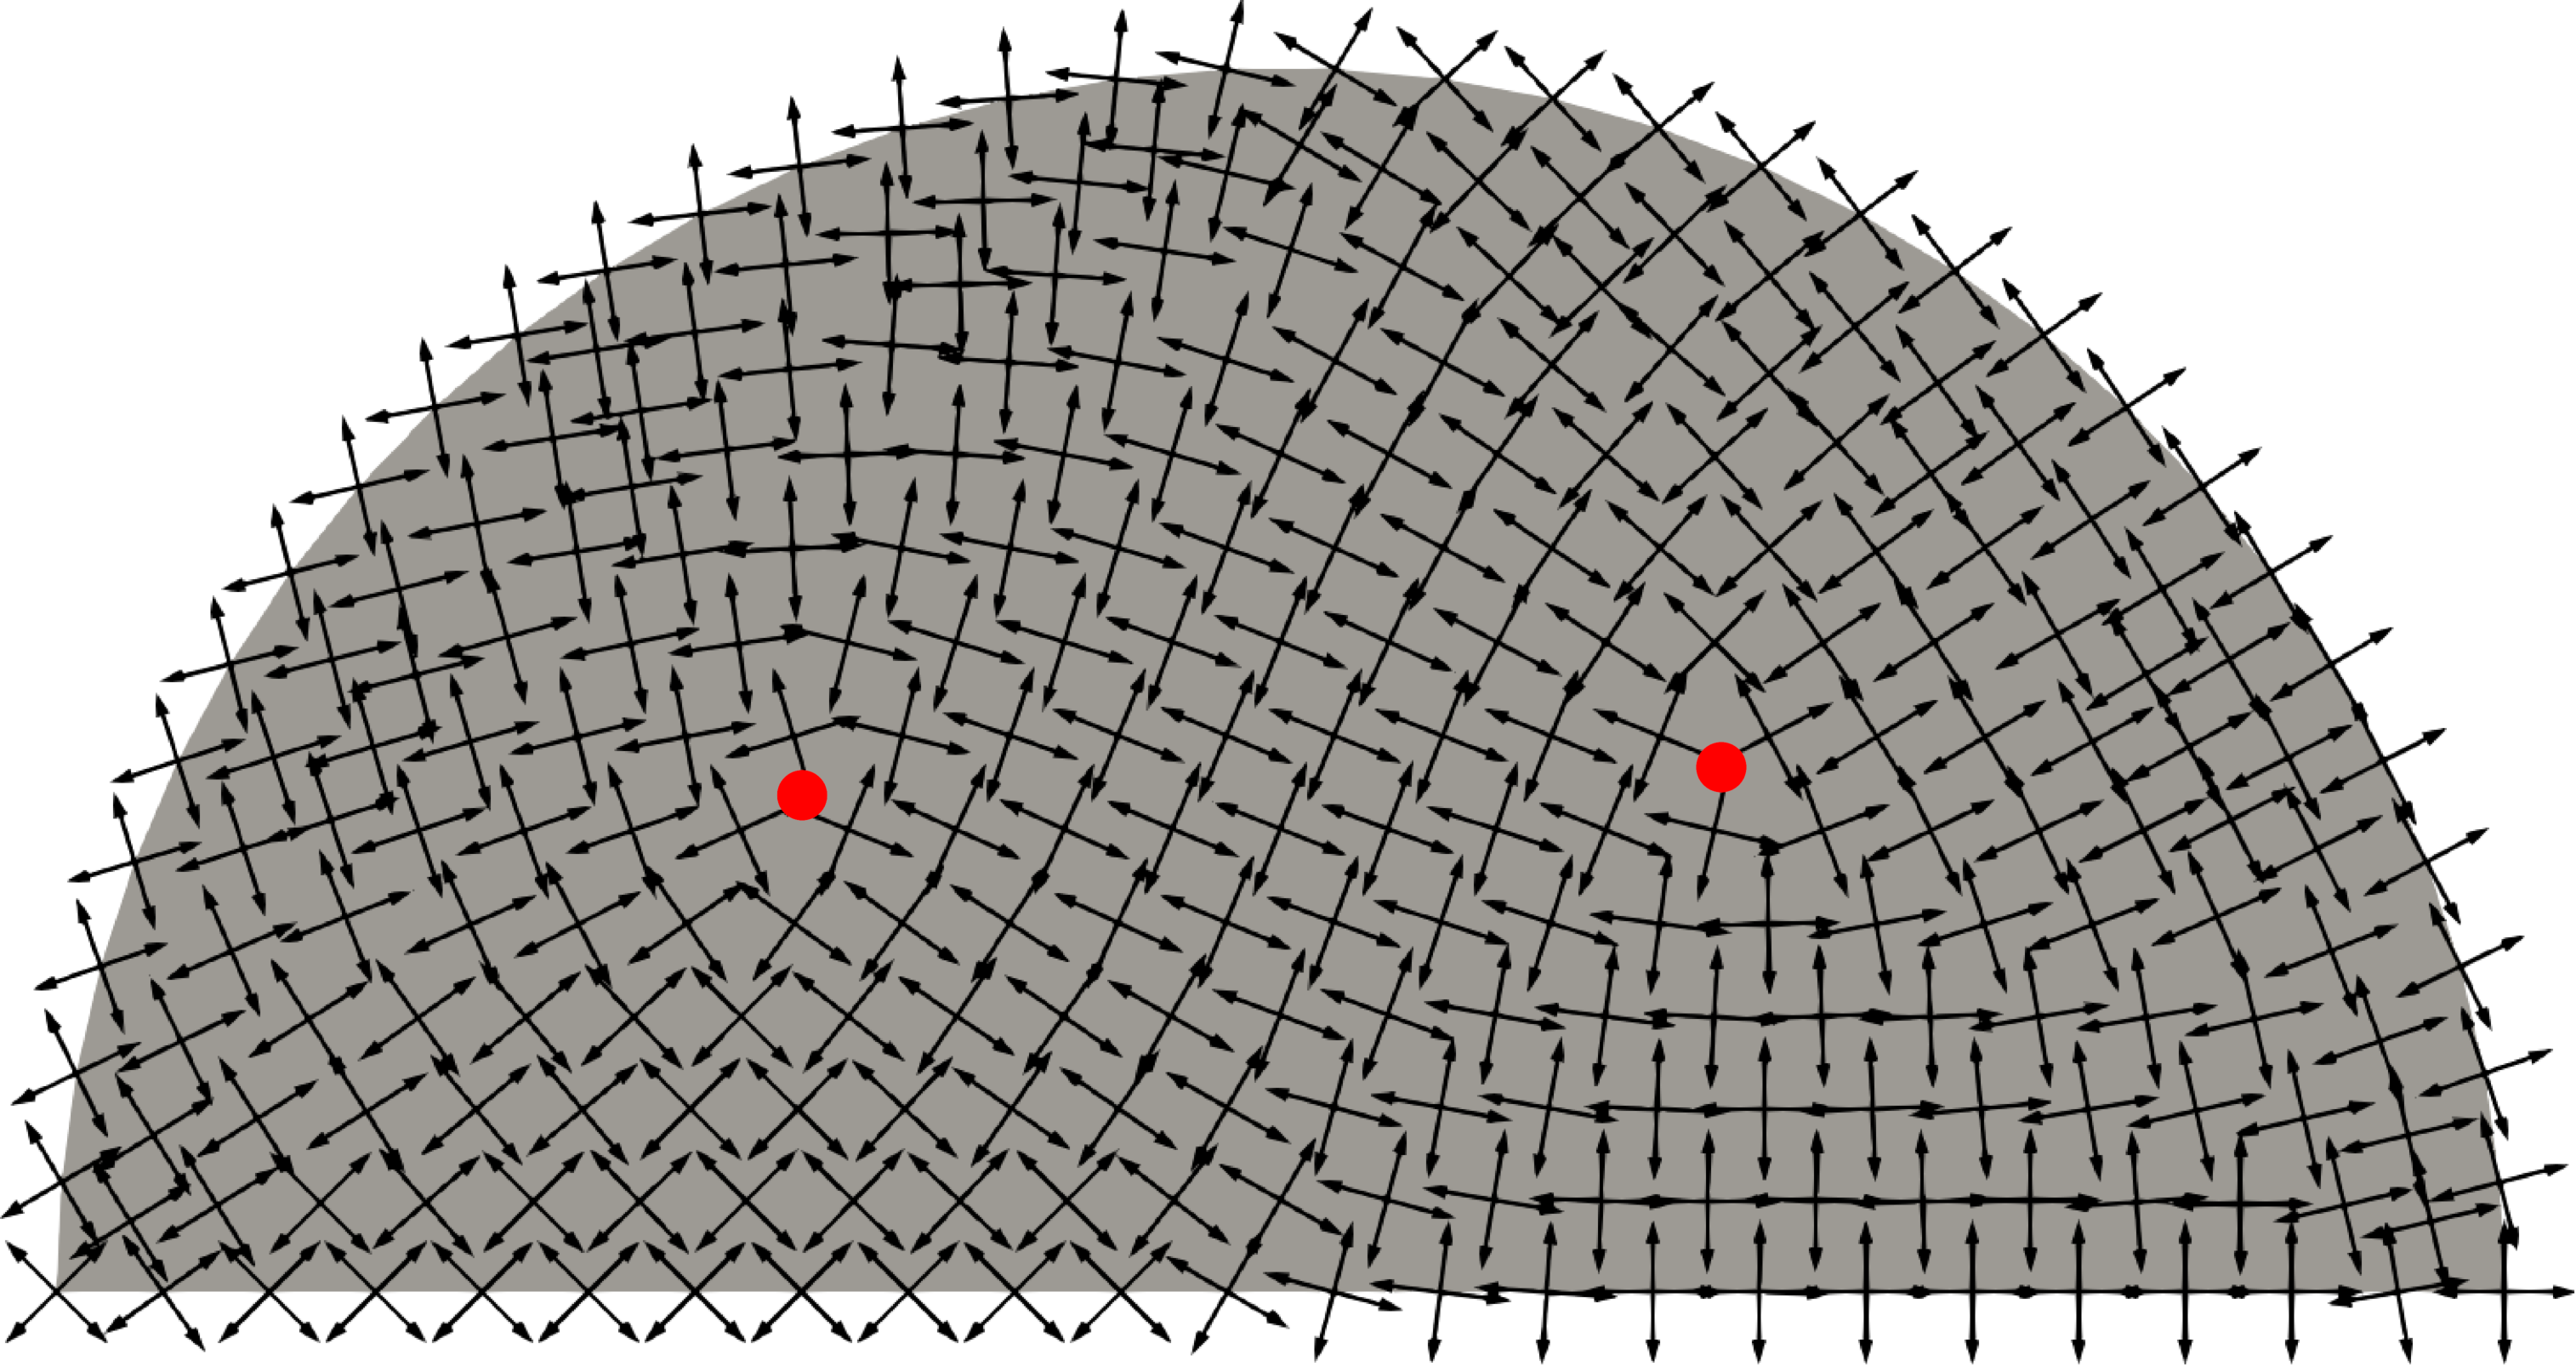
\includegraphics[scale=0.092]{images/mode_prop_cross_beam.pdf} \hspace{0.2cm}
        %\footnotesize Cross-field
        }
\only<4>{
        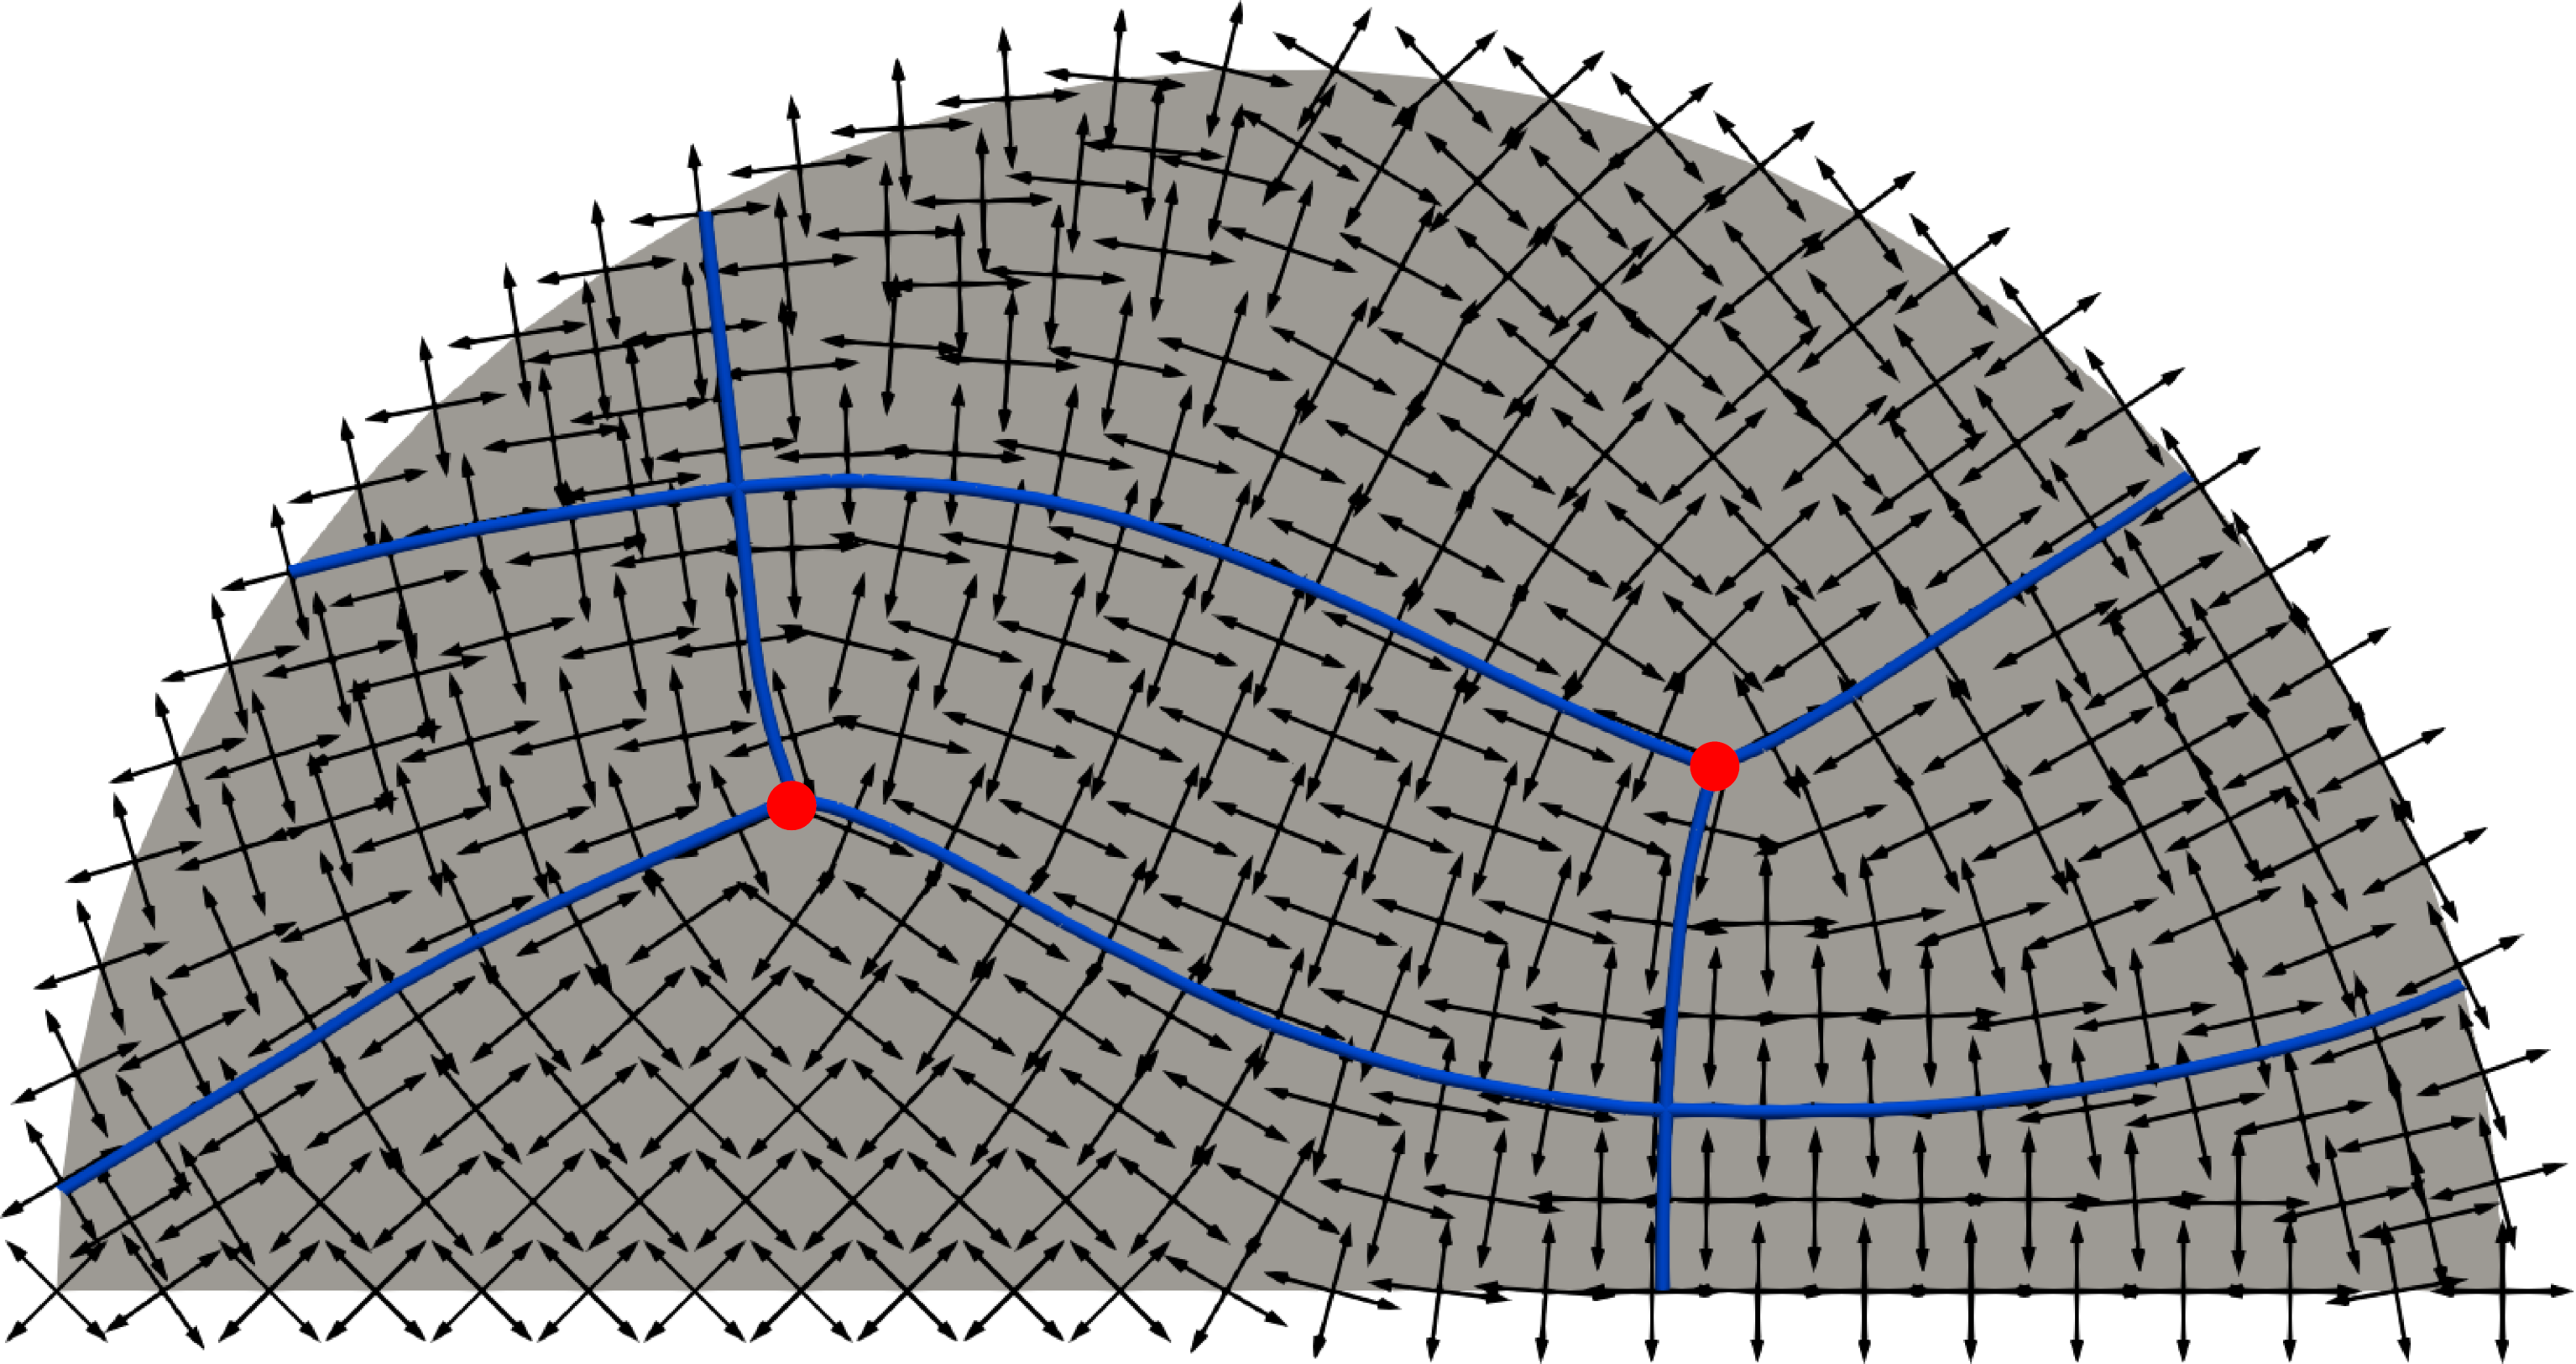
\includegraphics[scale=0.092]{images/mode_prop_stream_non_align_beam.pdf} \hspace{0.2cm}
        %\footnotesize Cross-field
        }
        \end{column}
    \end{columns}

\end{frame}


%\begin{frame}{Prise en compte de champs de croix arbitraires}

%    \begin{columns}
%        \begin{column}{0.33\textwidth}
%        \centering
%\onslide<1->{
%        %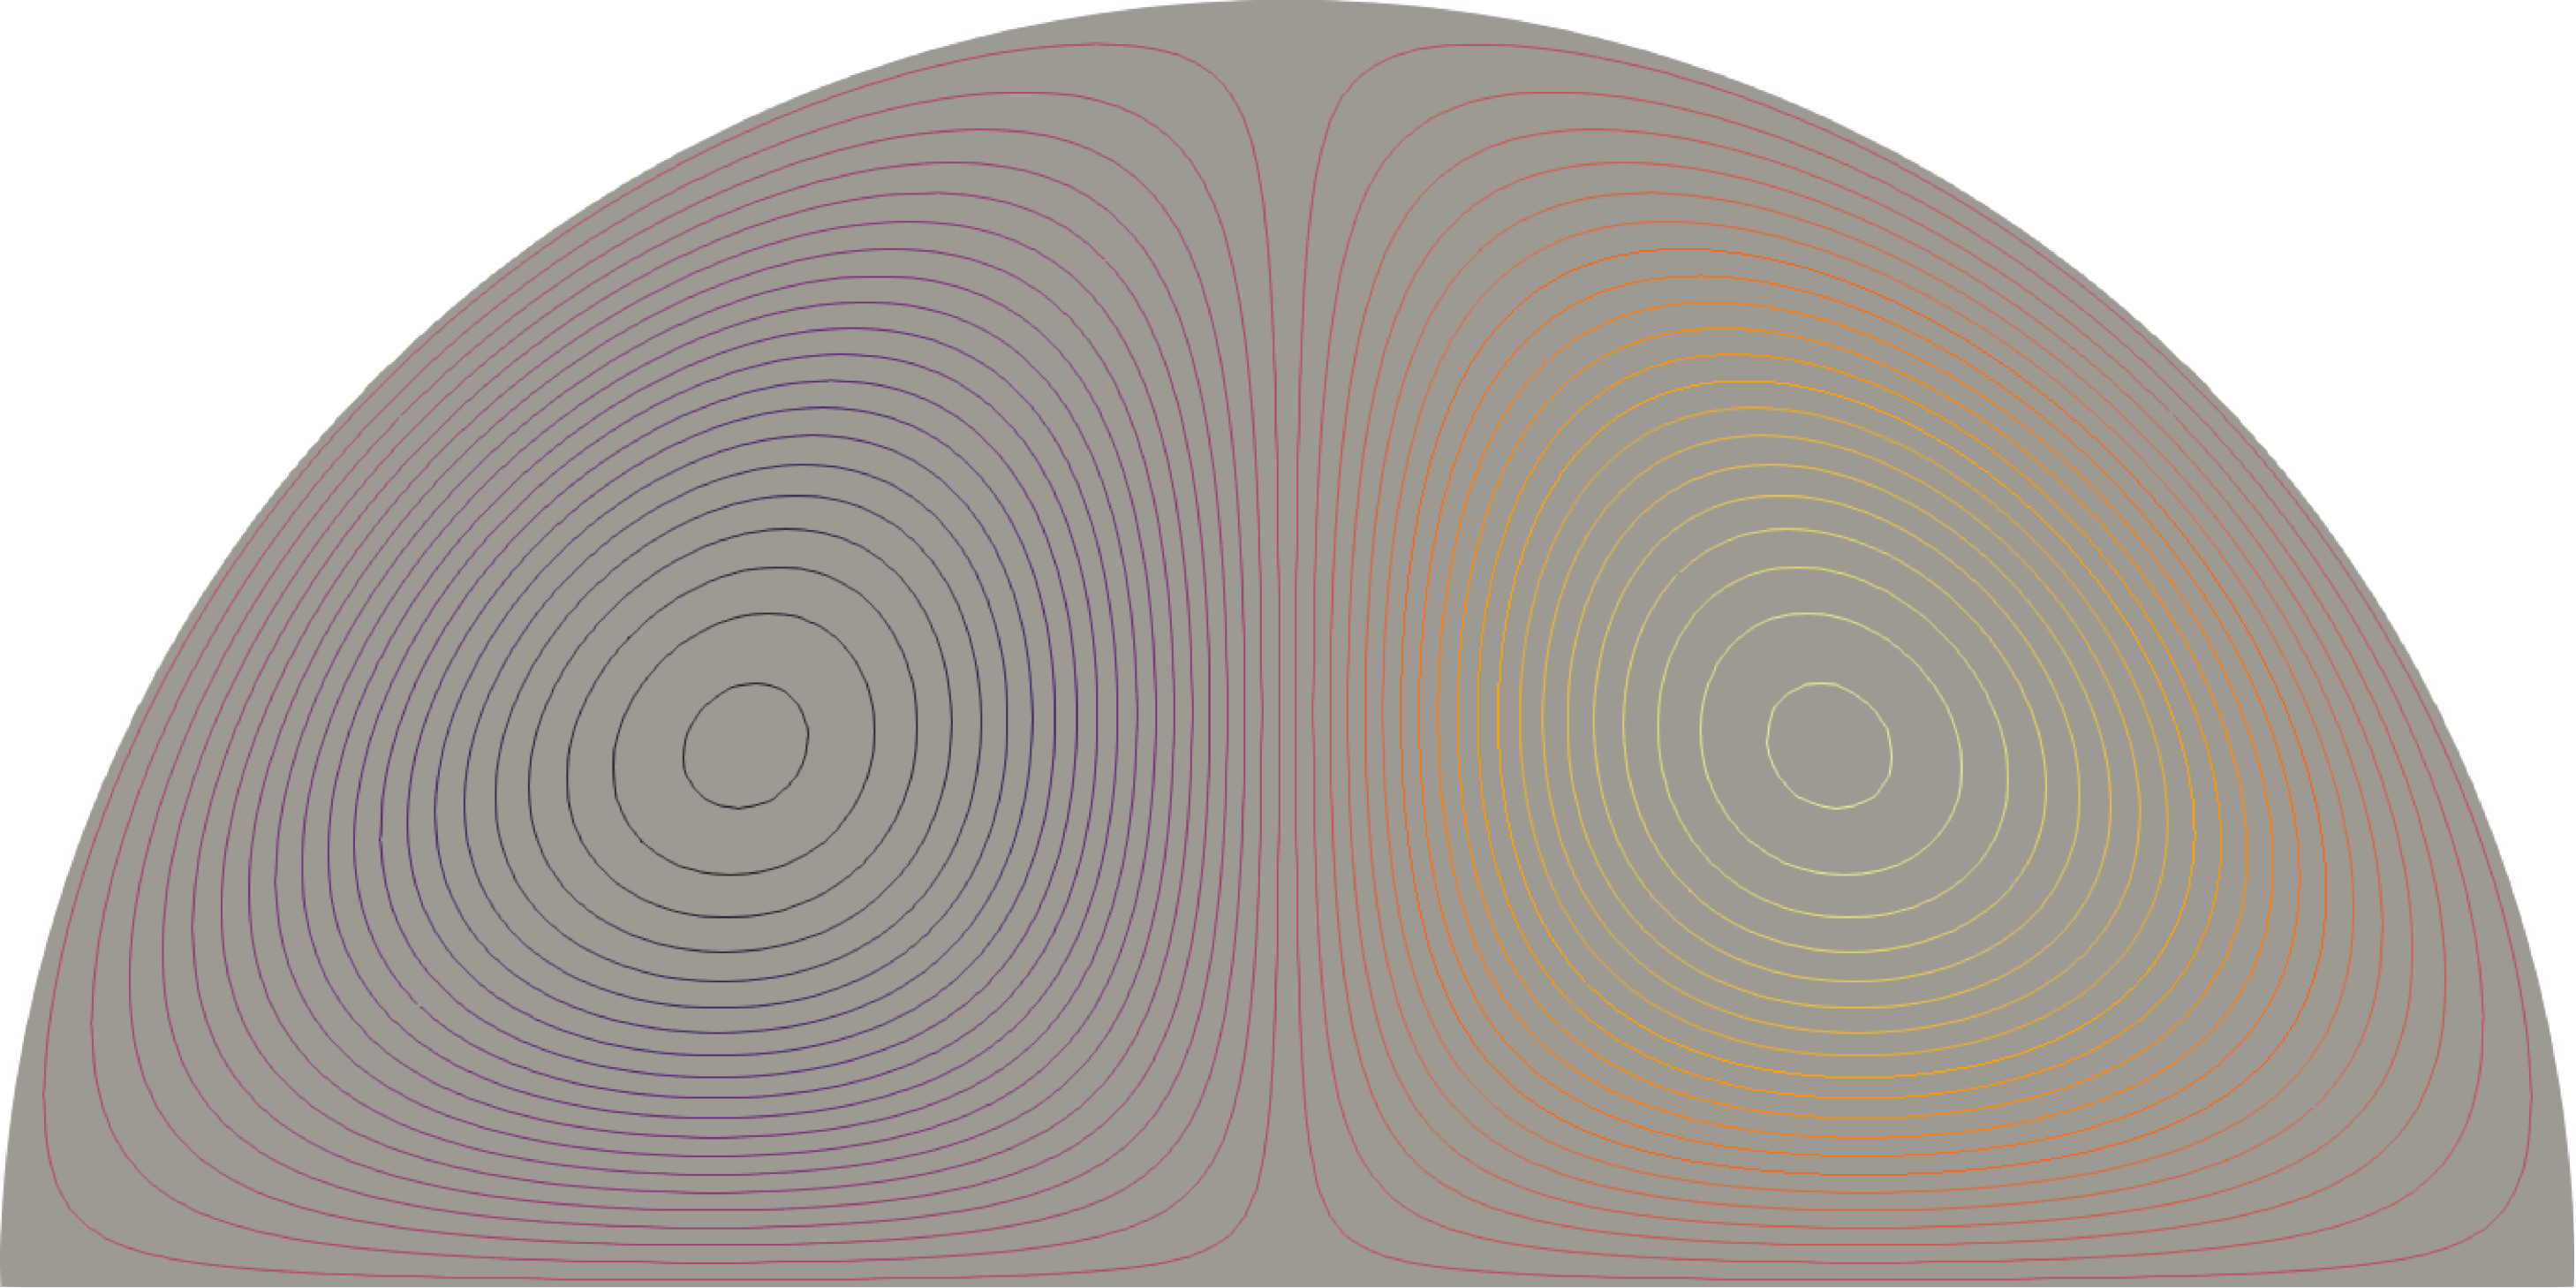
\includegraphics[scale=0.091]{images/mode_prop.pdf}
%        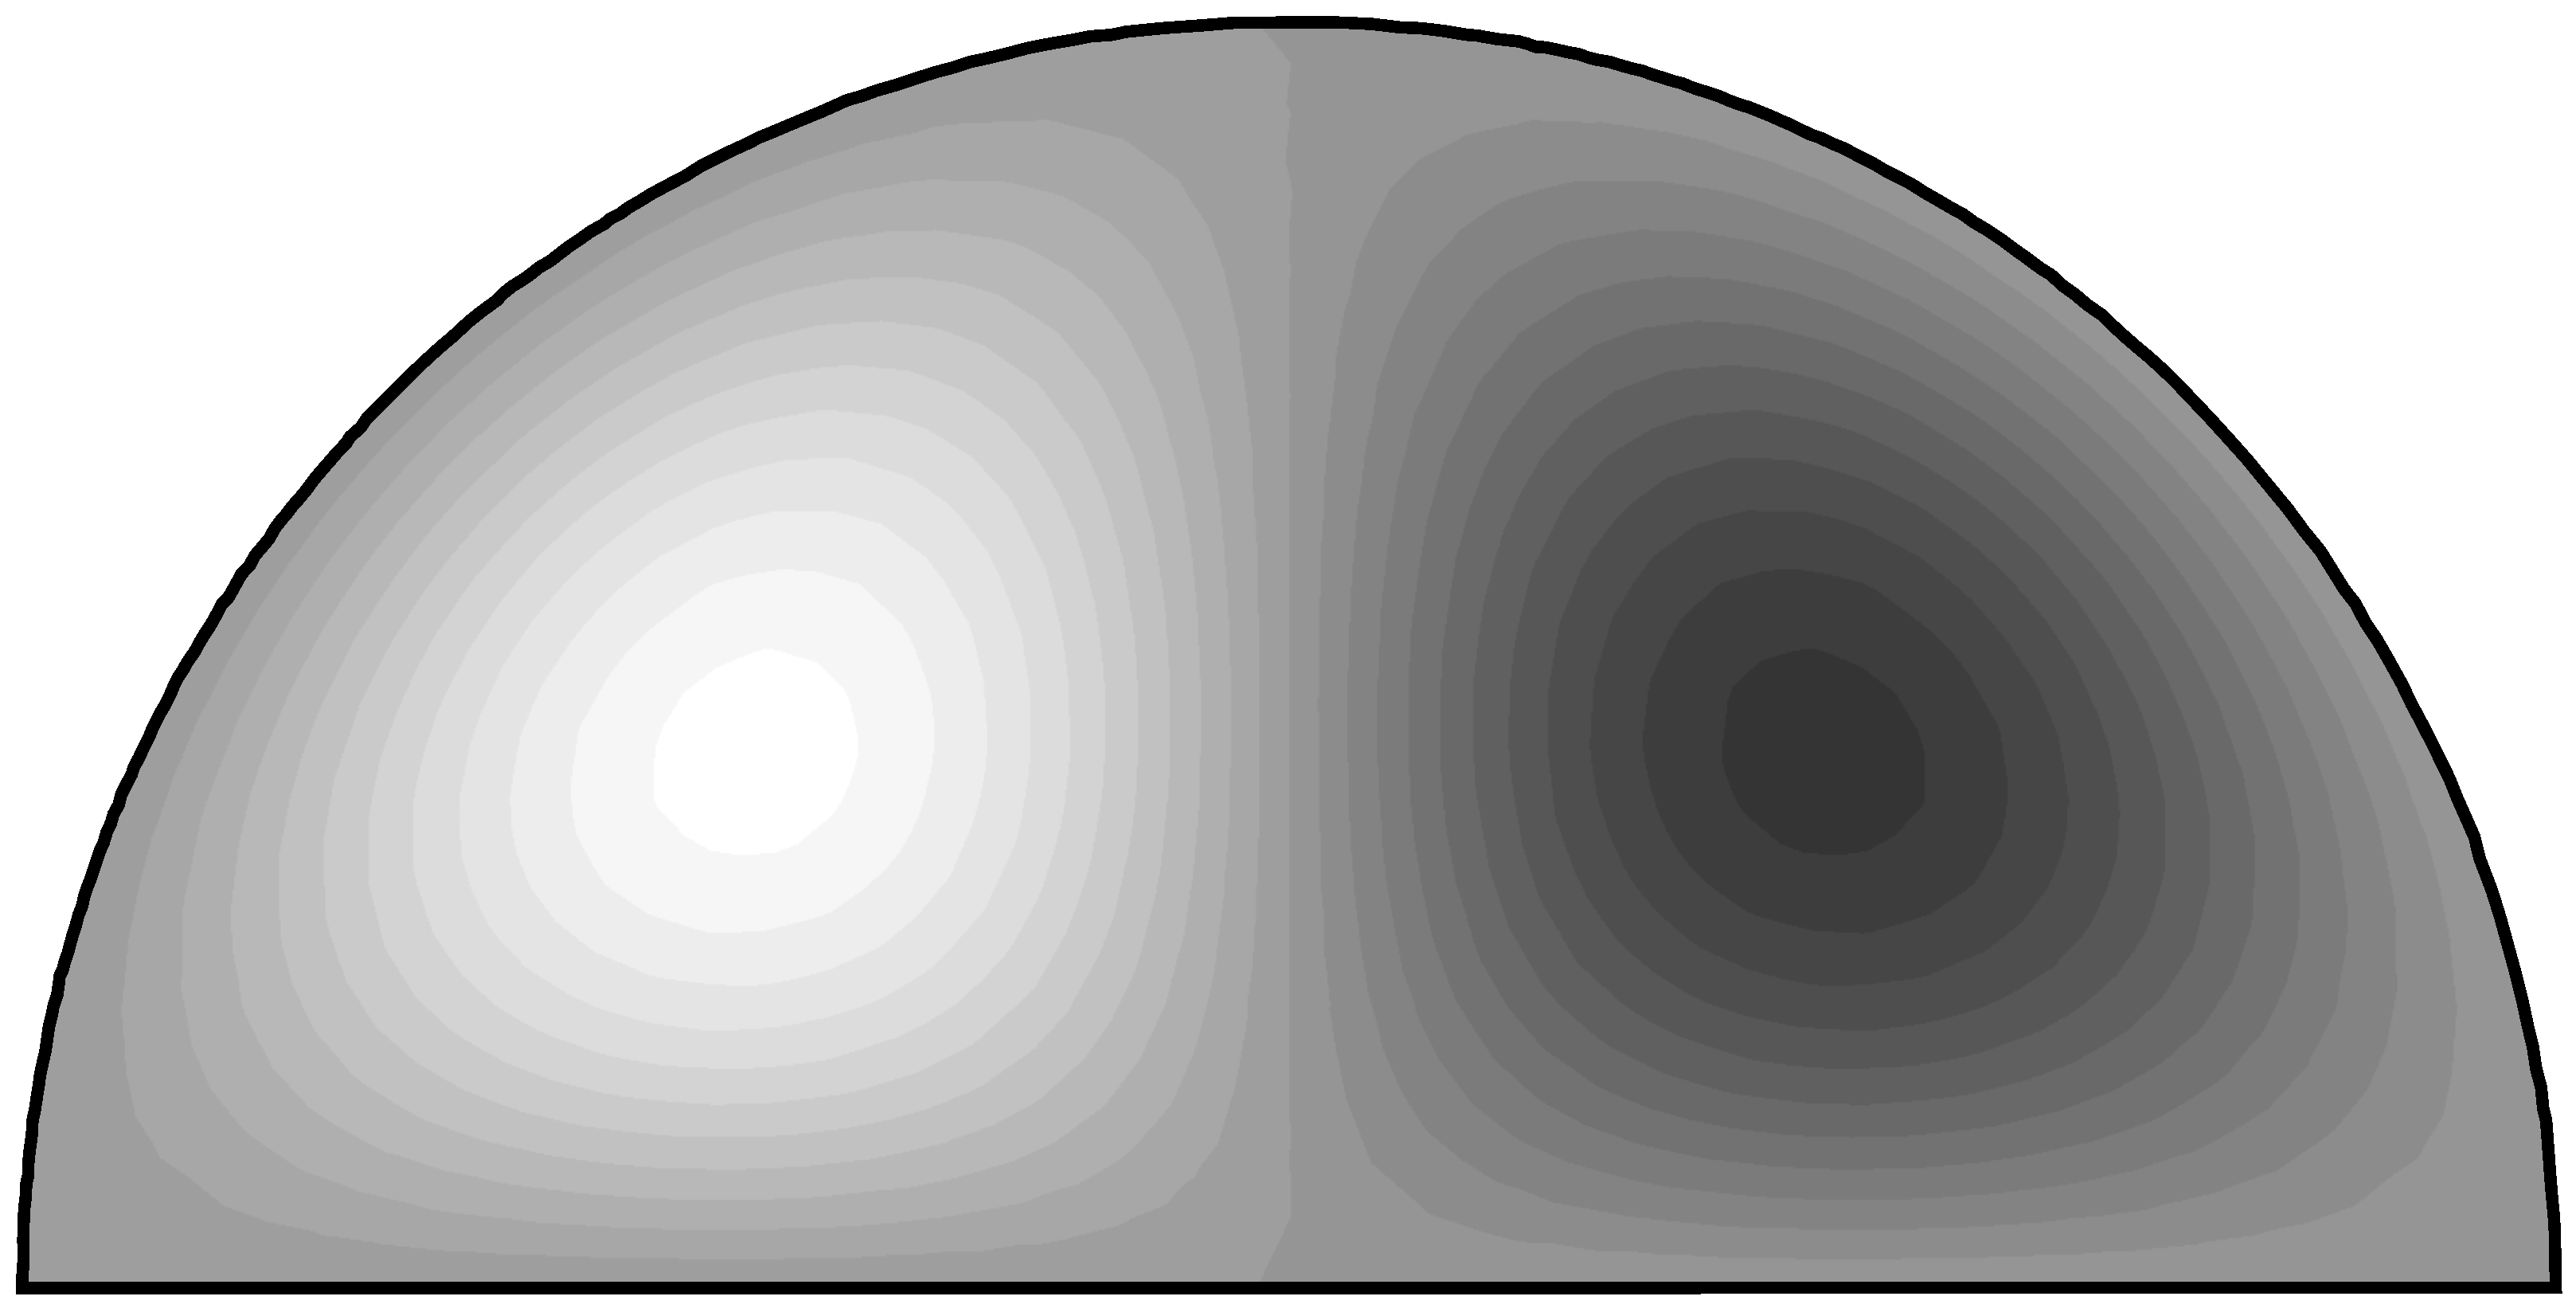
\includegraphics[scale=0.085]{images/demiDiscValProp.eps} \hspace{0.2cm}
%        \footnotesize Mode propre sur le demi-disque}
%        \end{column}
%        \begin{column}{0.33\textwidth}
%        \centering
%\onslide<2->{
%        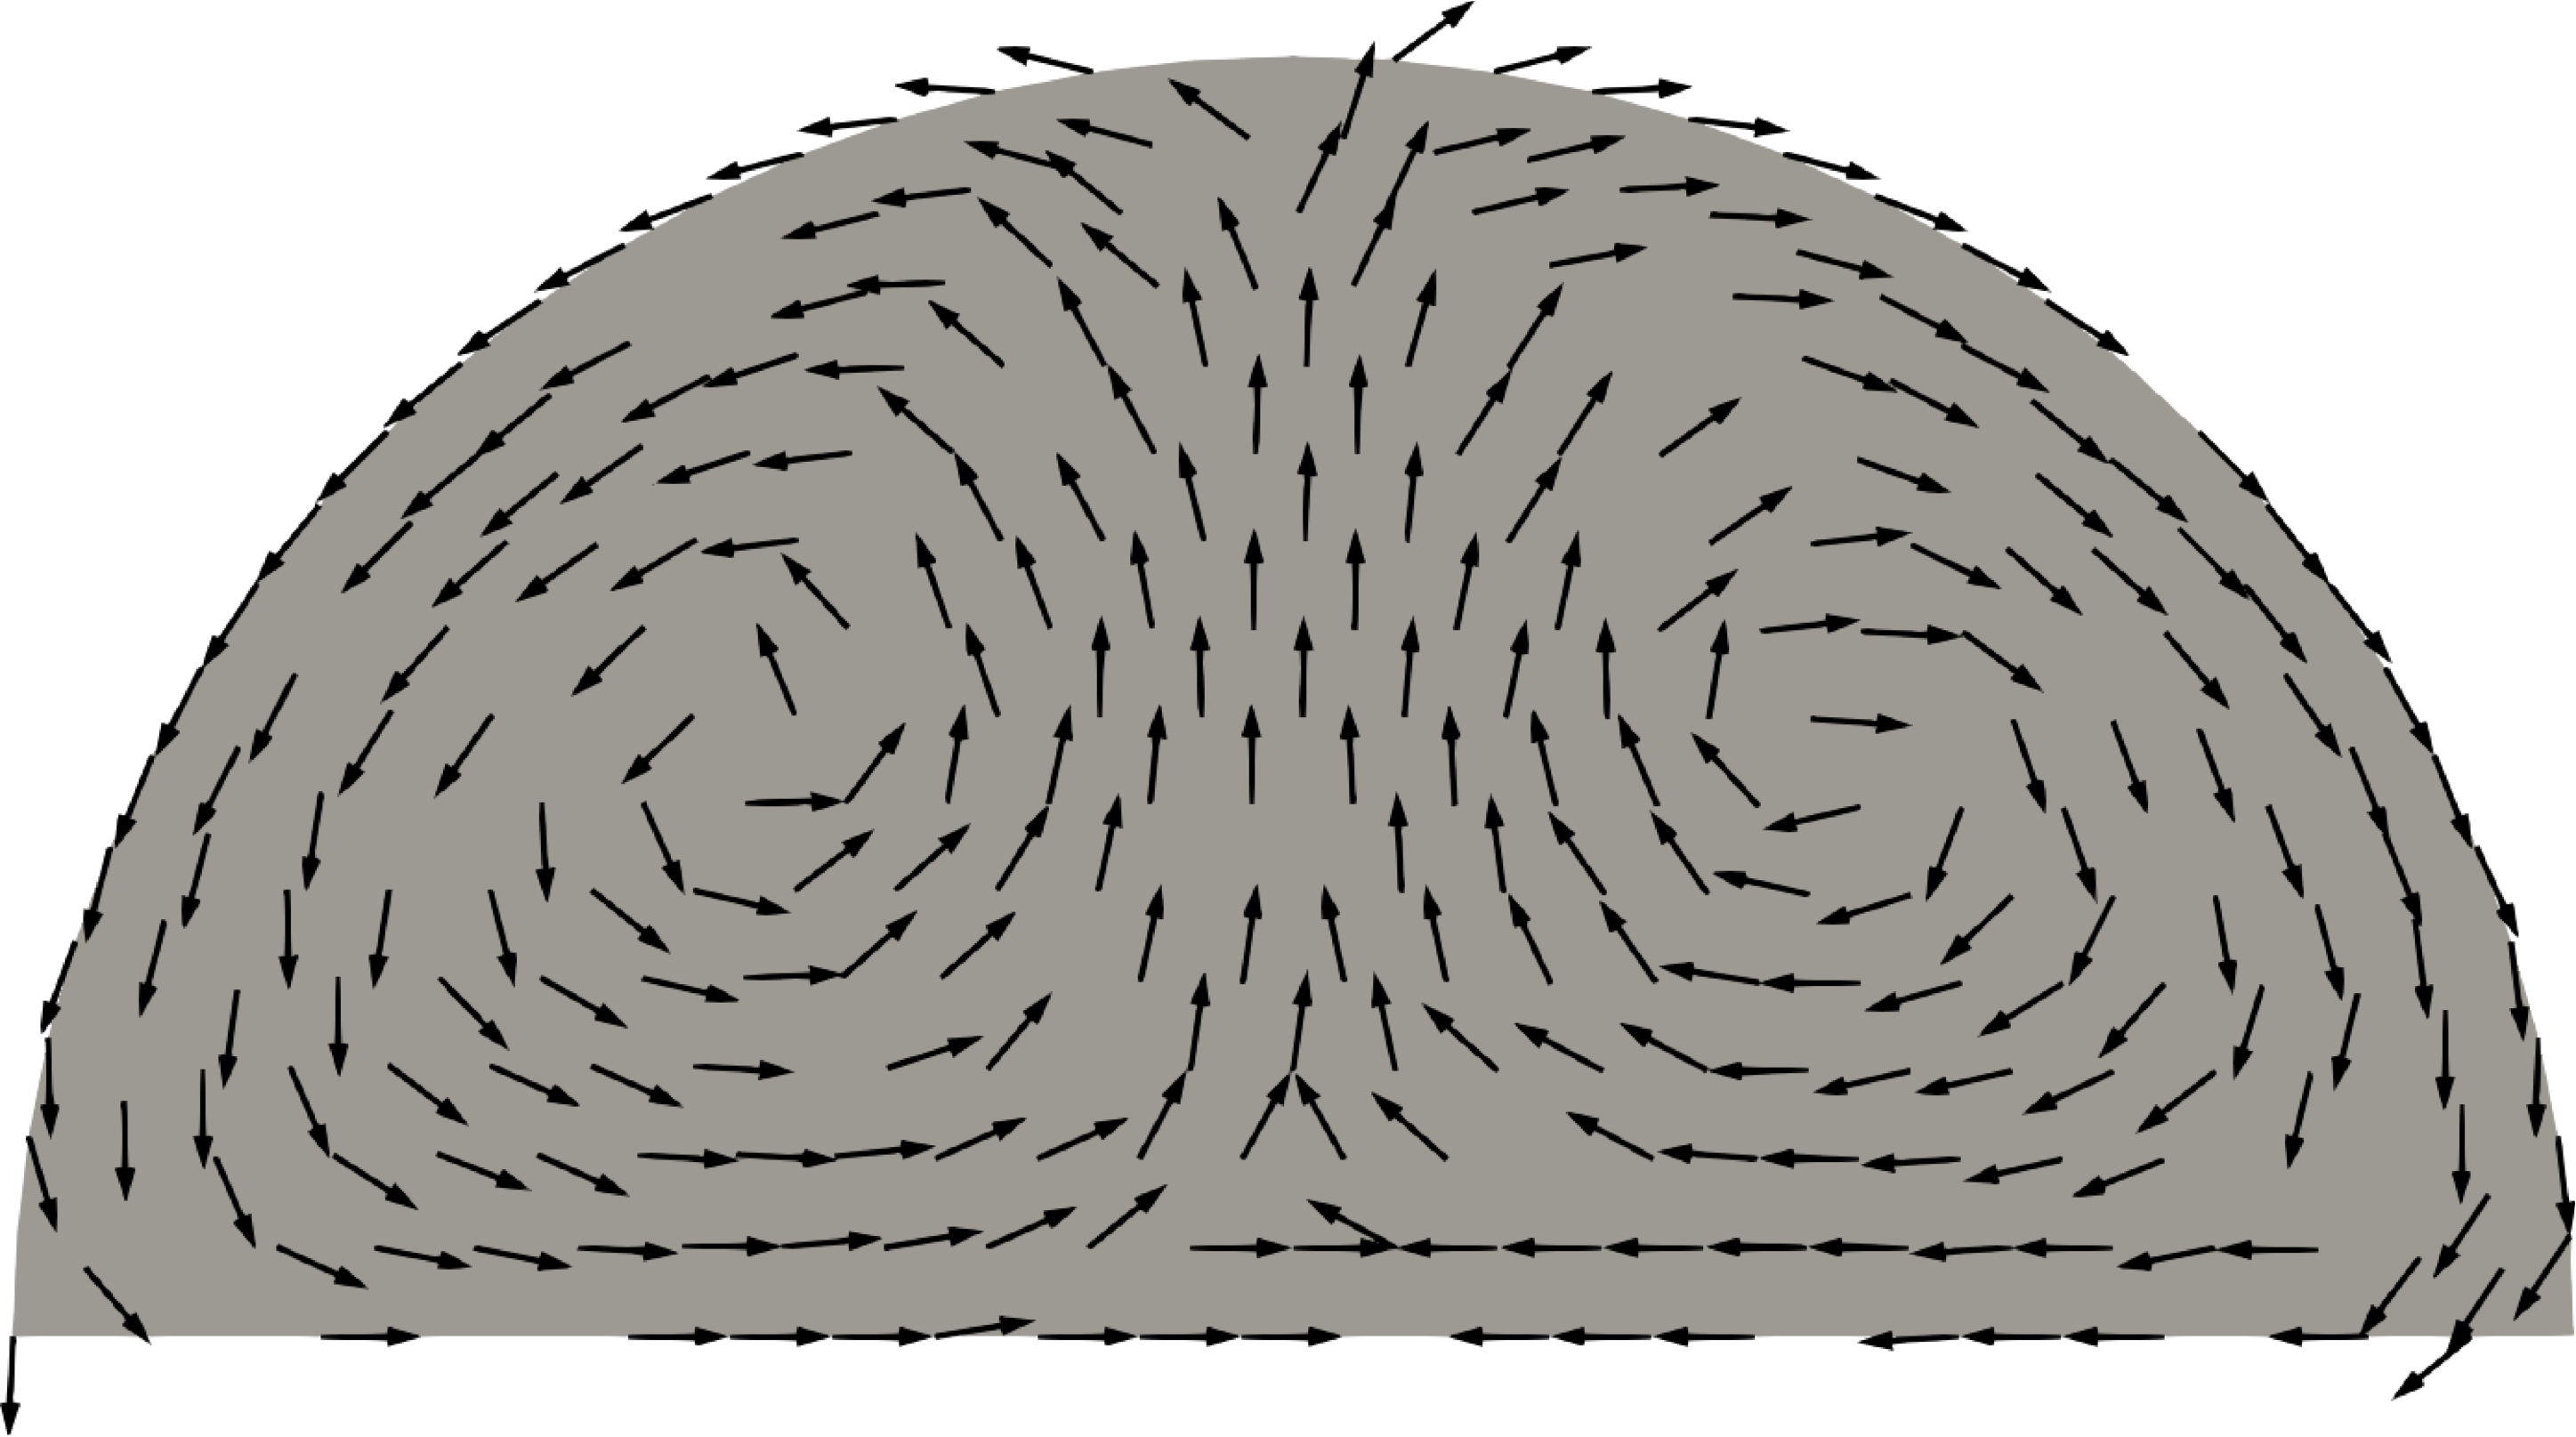
\includegraphics[scale=0.085]{images/iso_tangente.pdf} %\hspace{0.2cm}
%        \footnotesize Tangentes aux lignes de niveaux}
%        \end{column}
%        \begin{column}{0.33\textwidth}
%        \centering
%\onslide<3->{
%        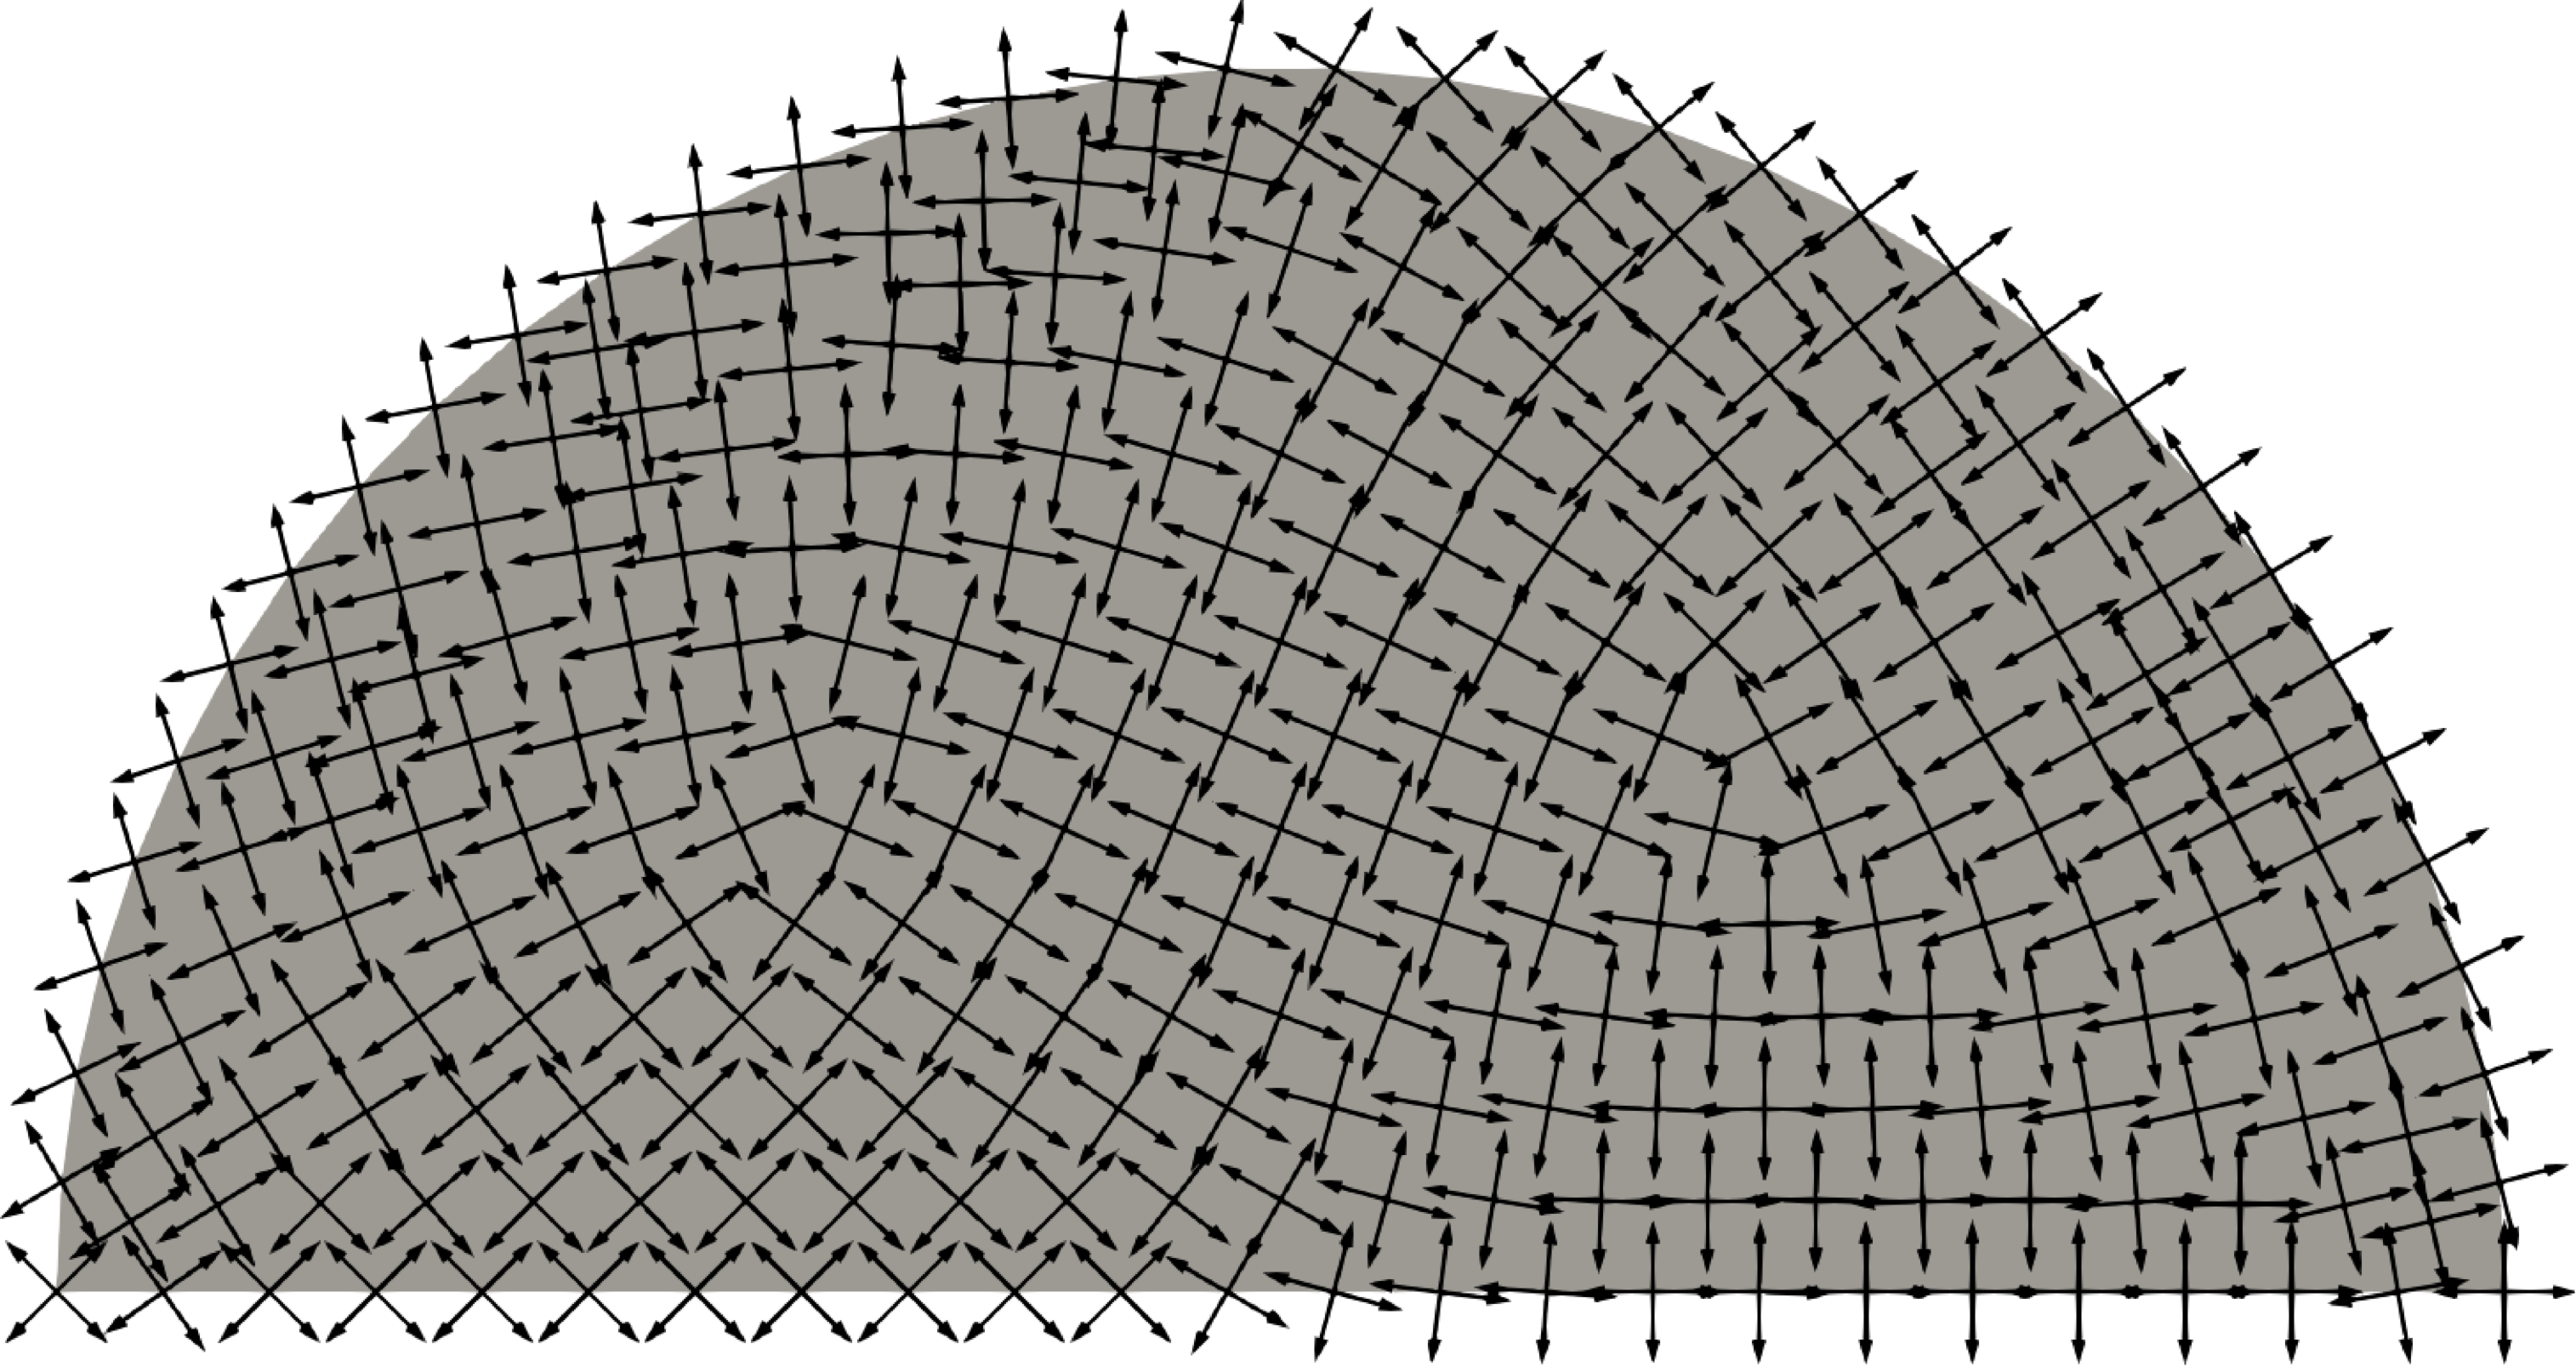
\includegraphics[scale=0.085]{images/mode_prop_cross.pdf} \hspace{0.2cm}
%        \footnotesize Champ de croix}
%        \end{column}
%    \end{columns}

%    \begin{columns}
%\onslide<5->{
%        \begin{column}{0.5\textwidth}

%        \begin{itemize}
%            \item Comment montrer q'une partition donnée est de quatres côtés ?\\\vspace{0.2cm}
%            \item Analyse du comportement locale du champ aux voisinnages de points singuliers.\\\vspace{0.2cm}
%            %\item Exemples%\\\vspace{0.2cm}
%        \end{itemize}
%}
%    \vspace{0.5cm}
%        \end{column}
%        \begin{column}{0.5\textwidth}
%             \centering
%\onslide<4->{
%            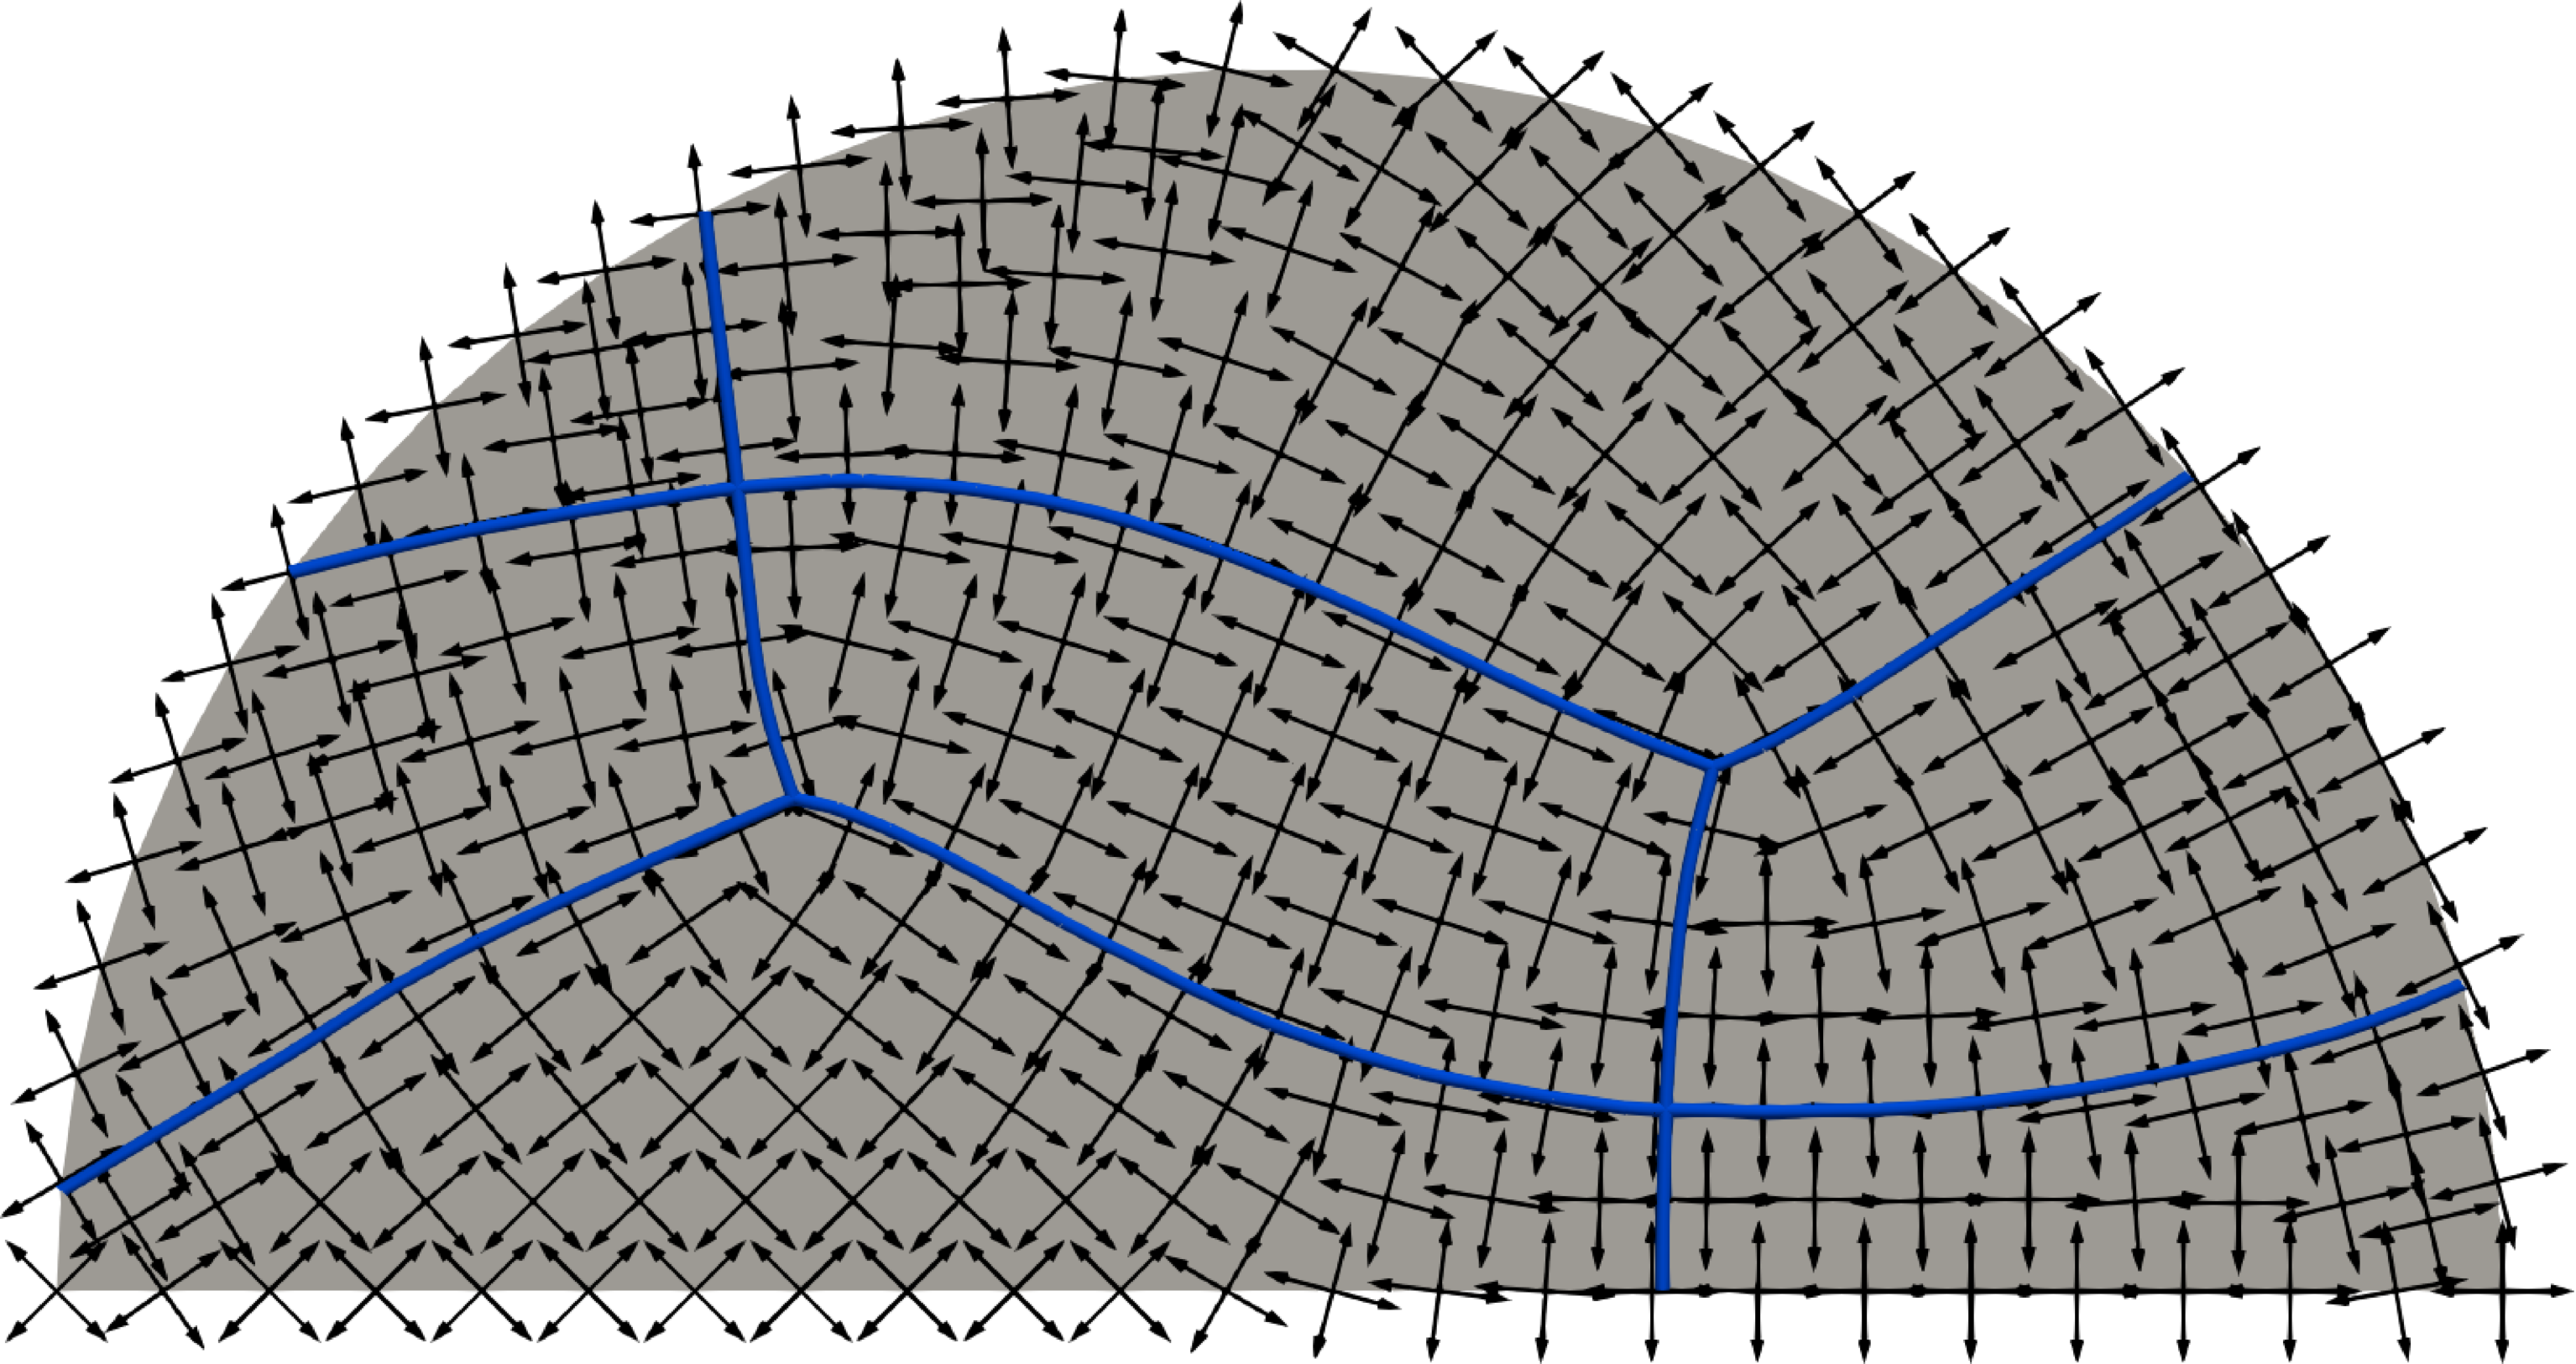
\includegraphics[scale=0.125]{images/mode_prop_stream_non_align.pdf}
%        }
%            %\hspace{0.2cm}
%            %\caption{\footnotesize Partitionnement}
%            \vspace{0.5cm}
%        \end{column}
%    \end{columns}
%\end{frame}

\begin{frame}{Handling Arbitrary Cross-Fields}
\small
\vspace{-0.2cm}
  \begin{columns}
    \begin{column}{0.7\textwidth}
{\bf What is a four-sided partition?}\\\vspace{0.2cm}
    {\color{onera} Index:} number of windings of the field around a point
\begin{itemize}
    \item if $p\in\Omega$ then $id_{\bar{u}}(p) = \frac{1}{2\pi}\int_\gamma d\theta_{\bar{u}}$
    \item if $p\in\partial\Omega$ then $id^\partial_{\bar{u}}(p)=\frac{1}{2\pi}\left[\pi-\hat{p}+\lim\limits_{s\rightarrow 0}\int_s^{1-s}d\theta_{\bar{u}}^\gamma\right]$
\end{itemize}
{\color{onera} Valence:} number of separatrices associated with a point
\begin{itemize}
    \item if $p\in\Omega$ then $N_s(p) = 4-4id_{\bar{u}}(p)$
    \item if $p\in\partial\Omega$ then $N_s(p) = 3-4id^\partial_{\bar{u}}(p)$
\end{itemize}
{\bf Example:} (See figure)\\\vspace{0.1cm}
\begin{onerablock}[drop fuzzy shadow]{\small  Lemma}
    \small The boundary index of a point (singular or intersection) with respect to a given partition $\mathcal{P}$ is 1/4.
\end{onerablock}
    \end{column}
    \begin{column}{0.3\textwidth}
        \centering
  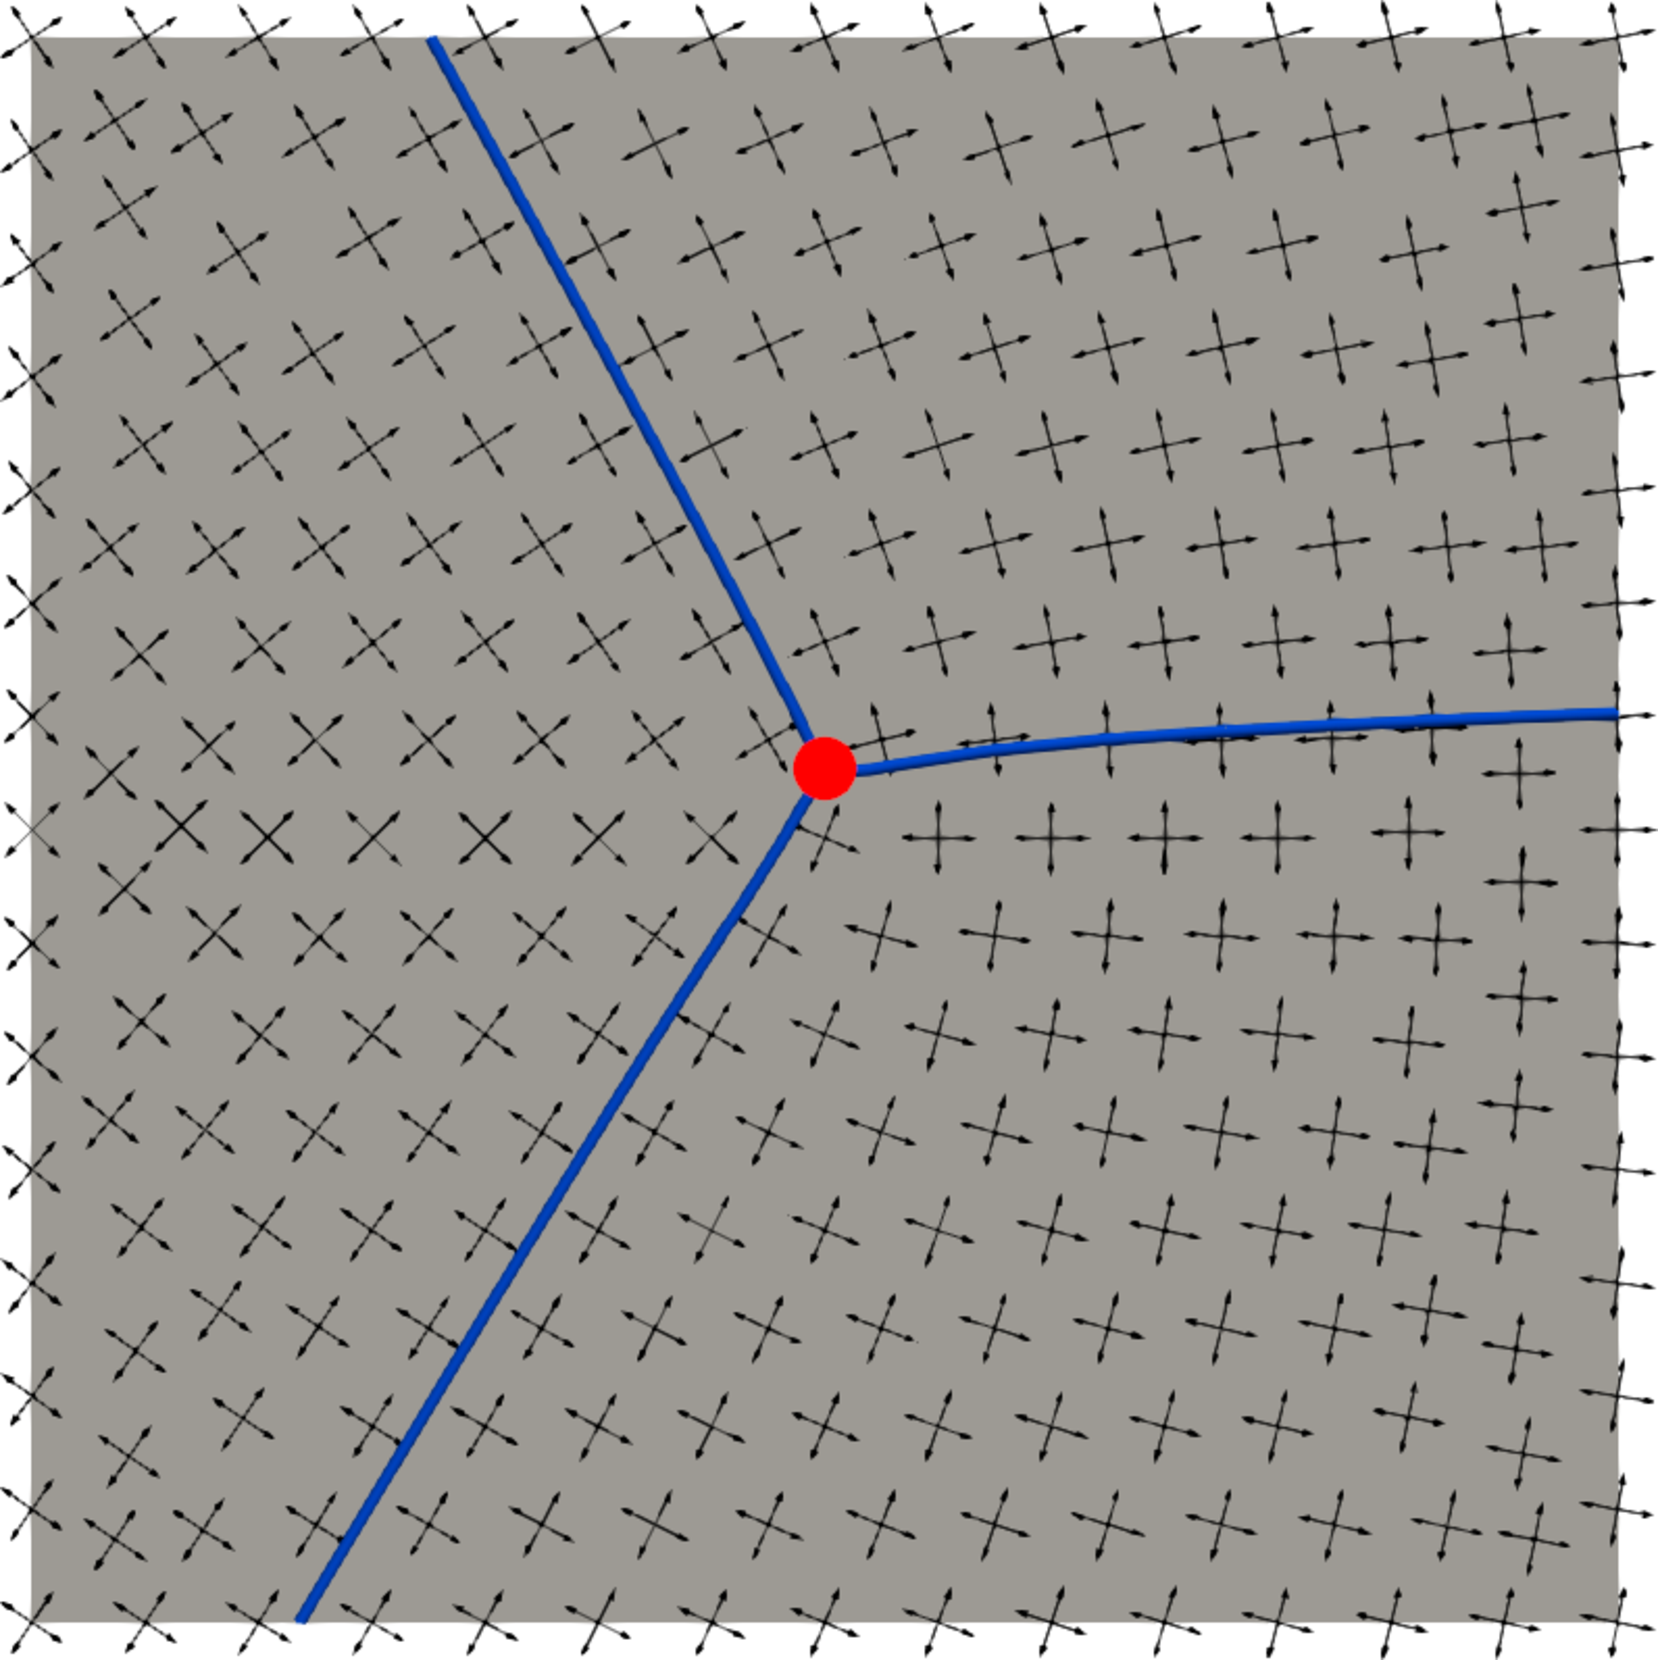
\includegraphics[scale=0.1]{images/sepa_3.pdf}
  \scriptsize $id_{\bar{u}}(p)=1/4, N_s(p) = 3$
  \\\vspace{0.1cm}
  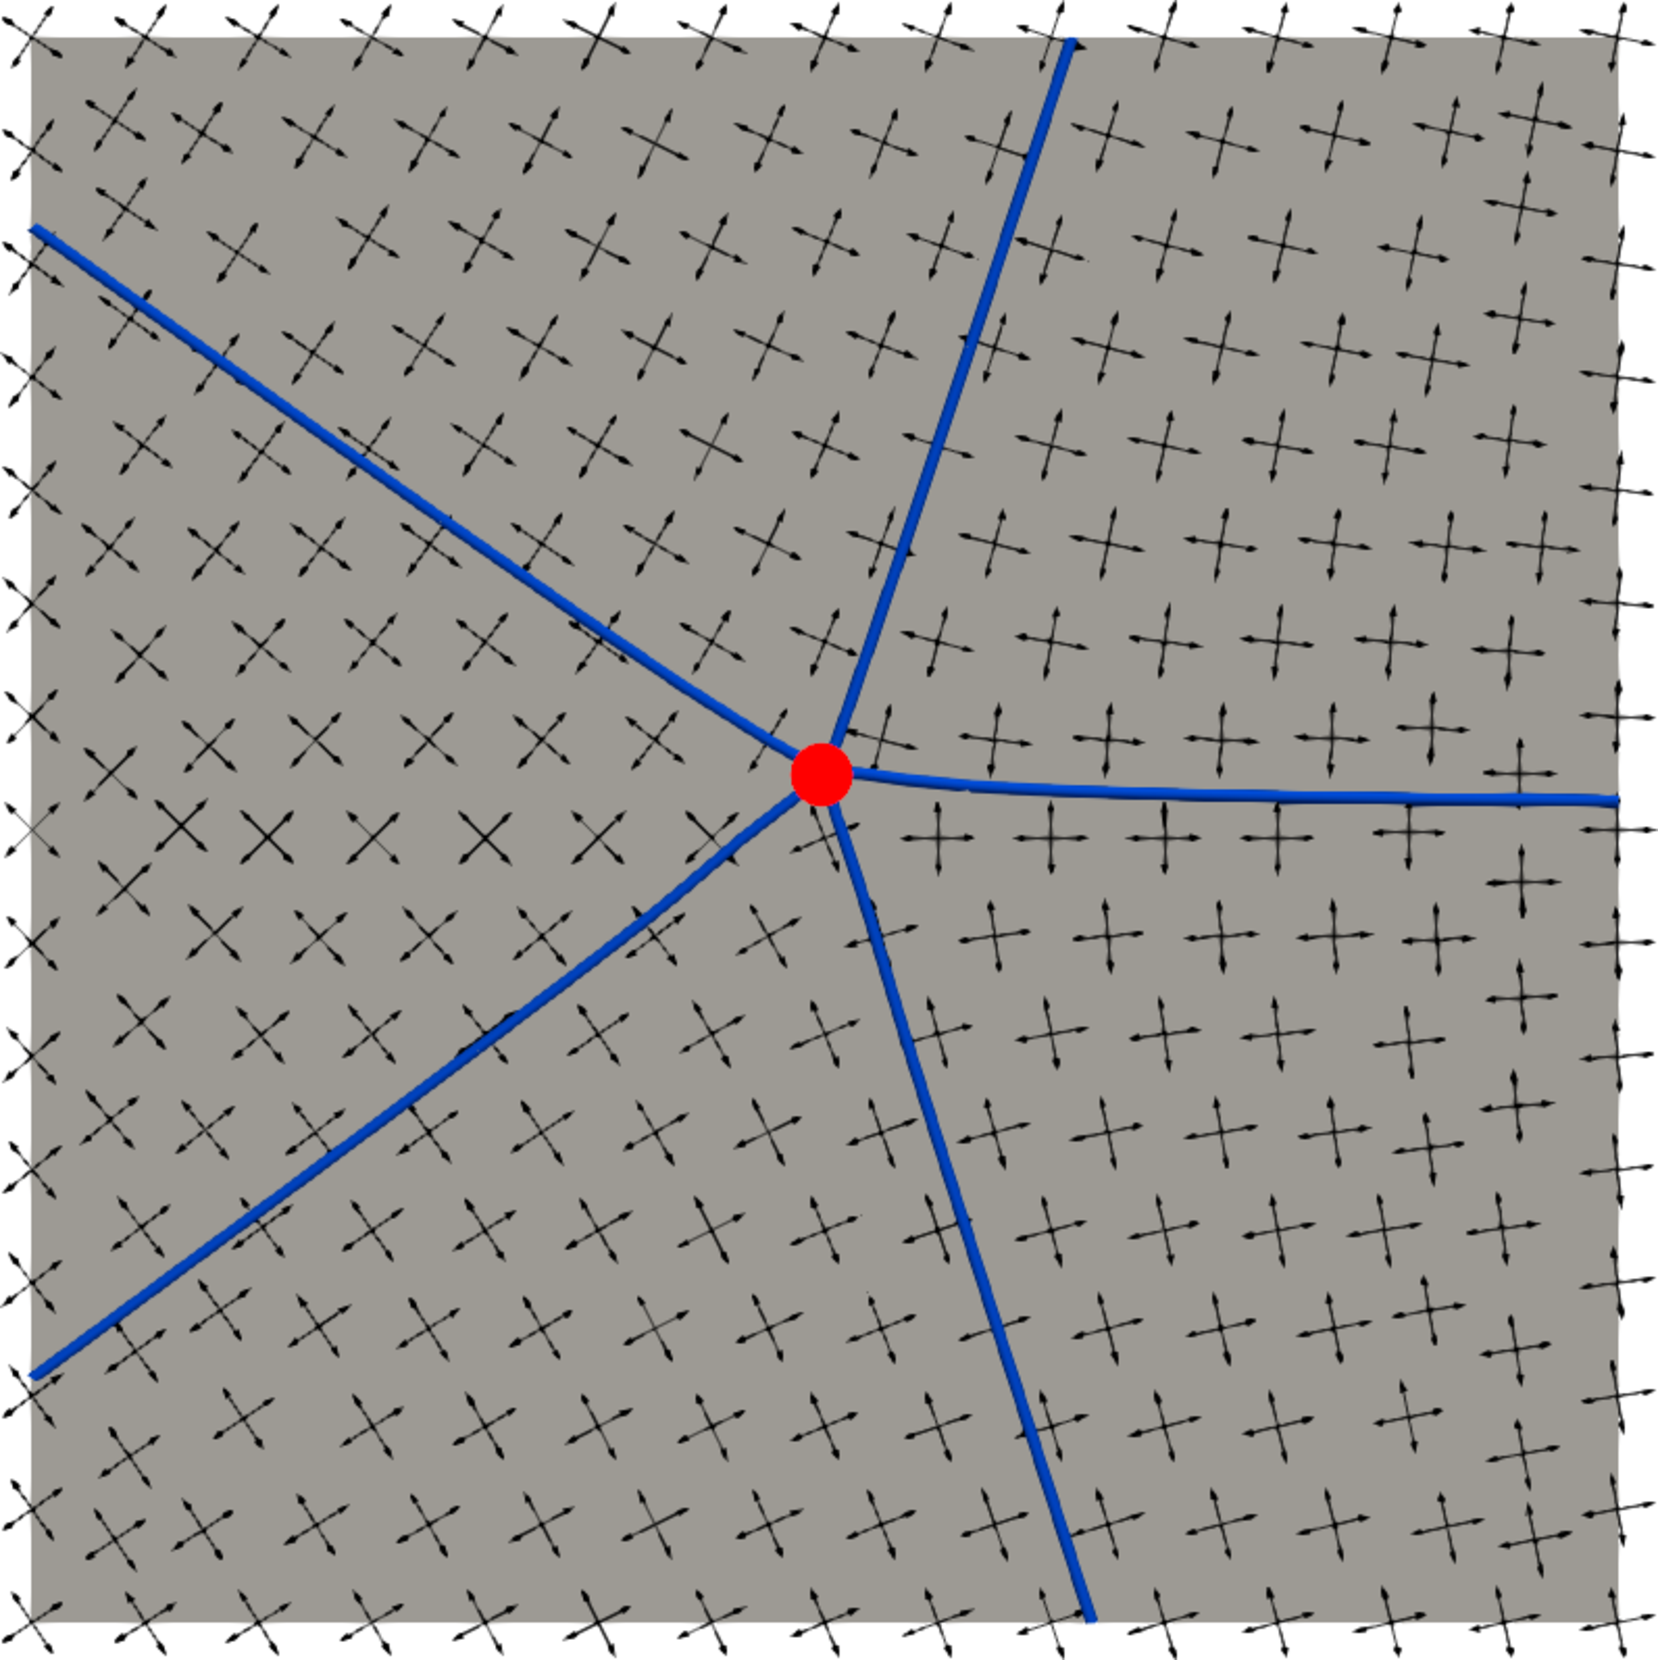
\includegraphics[scale=0.1]{images/sepa_5.pdf}
  \scriptsize $id_{\bar{u}}(p)=-1/4, N_s(p) = 5$
  \\\vspace{0.3cm}
    \end{column}
\end{columns}

\end{frame}


\begin{frame}{Handling Arbitrary Cross-Fields}%{How}
\small
\vspace{-0.2cm}
We exploit this result as follows: {\color{onera_gray} (formation of four-sided partitions)}\\\vspace{0.1cm}
Let $\mathcal{P}$ be any partition. {\color{onera_gray} (At this stage, we do not yet know its number of sides, blind separatrix)}
$$\chi(\mathcal{P})=1. \quad\quad{\color{onera_gray} (\chi=2-2g-b, g=0, b=1)}$$
By construction, the edges of the partition are aligned with the field, and it does not contain any internal singular points. The Poincaré-Hopf theorem then gives:
$$\chi(\mathcal{P})=\sum_{i=1}^{n_c}id_{\bar{u}}(c_i).$$
Combining, we get:
$$1=\sum_{i=1}^{n_c}\frac{1}{4}\Longrightarrow n_c=4.$$
\textbf{Conclusion:} Any partition whose edges are aligned with the field (separatrices) will have 4 sides.
\vspace{0.4cm}
\end{frame}

\begin{frame}{Handling Arbitrary Cross-Fields}{An Example of a Cross-Field Aligned with the Domain Boundary}

    \begin{columns}
        \begin{column}{0.33\textwidth}
        \centering
        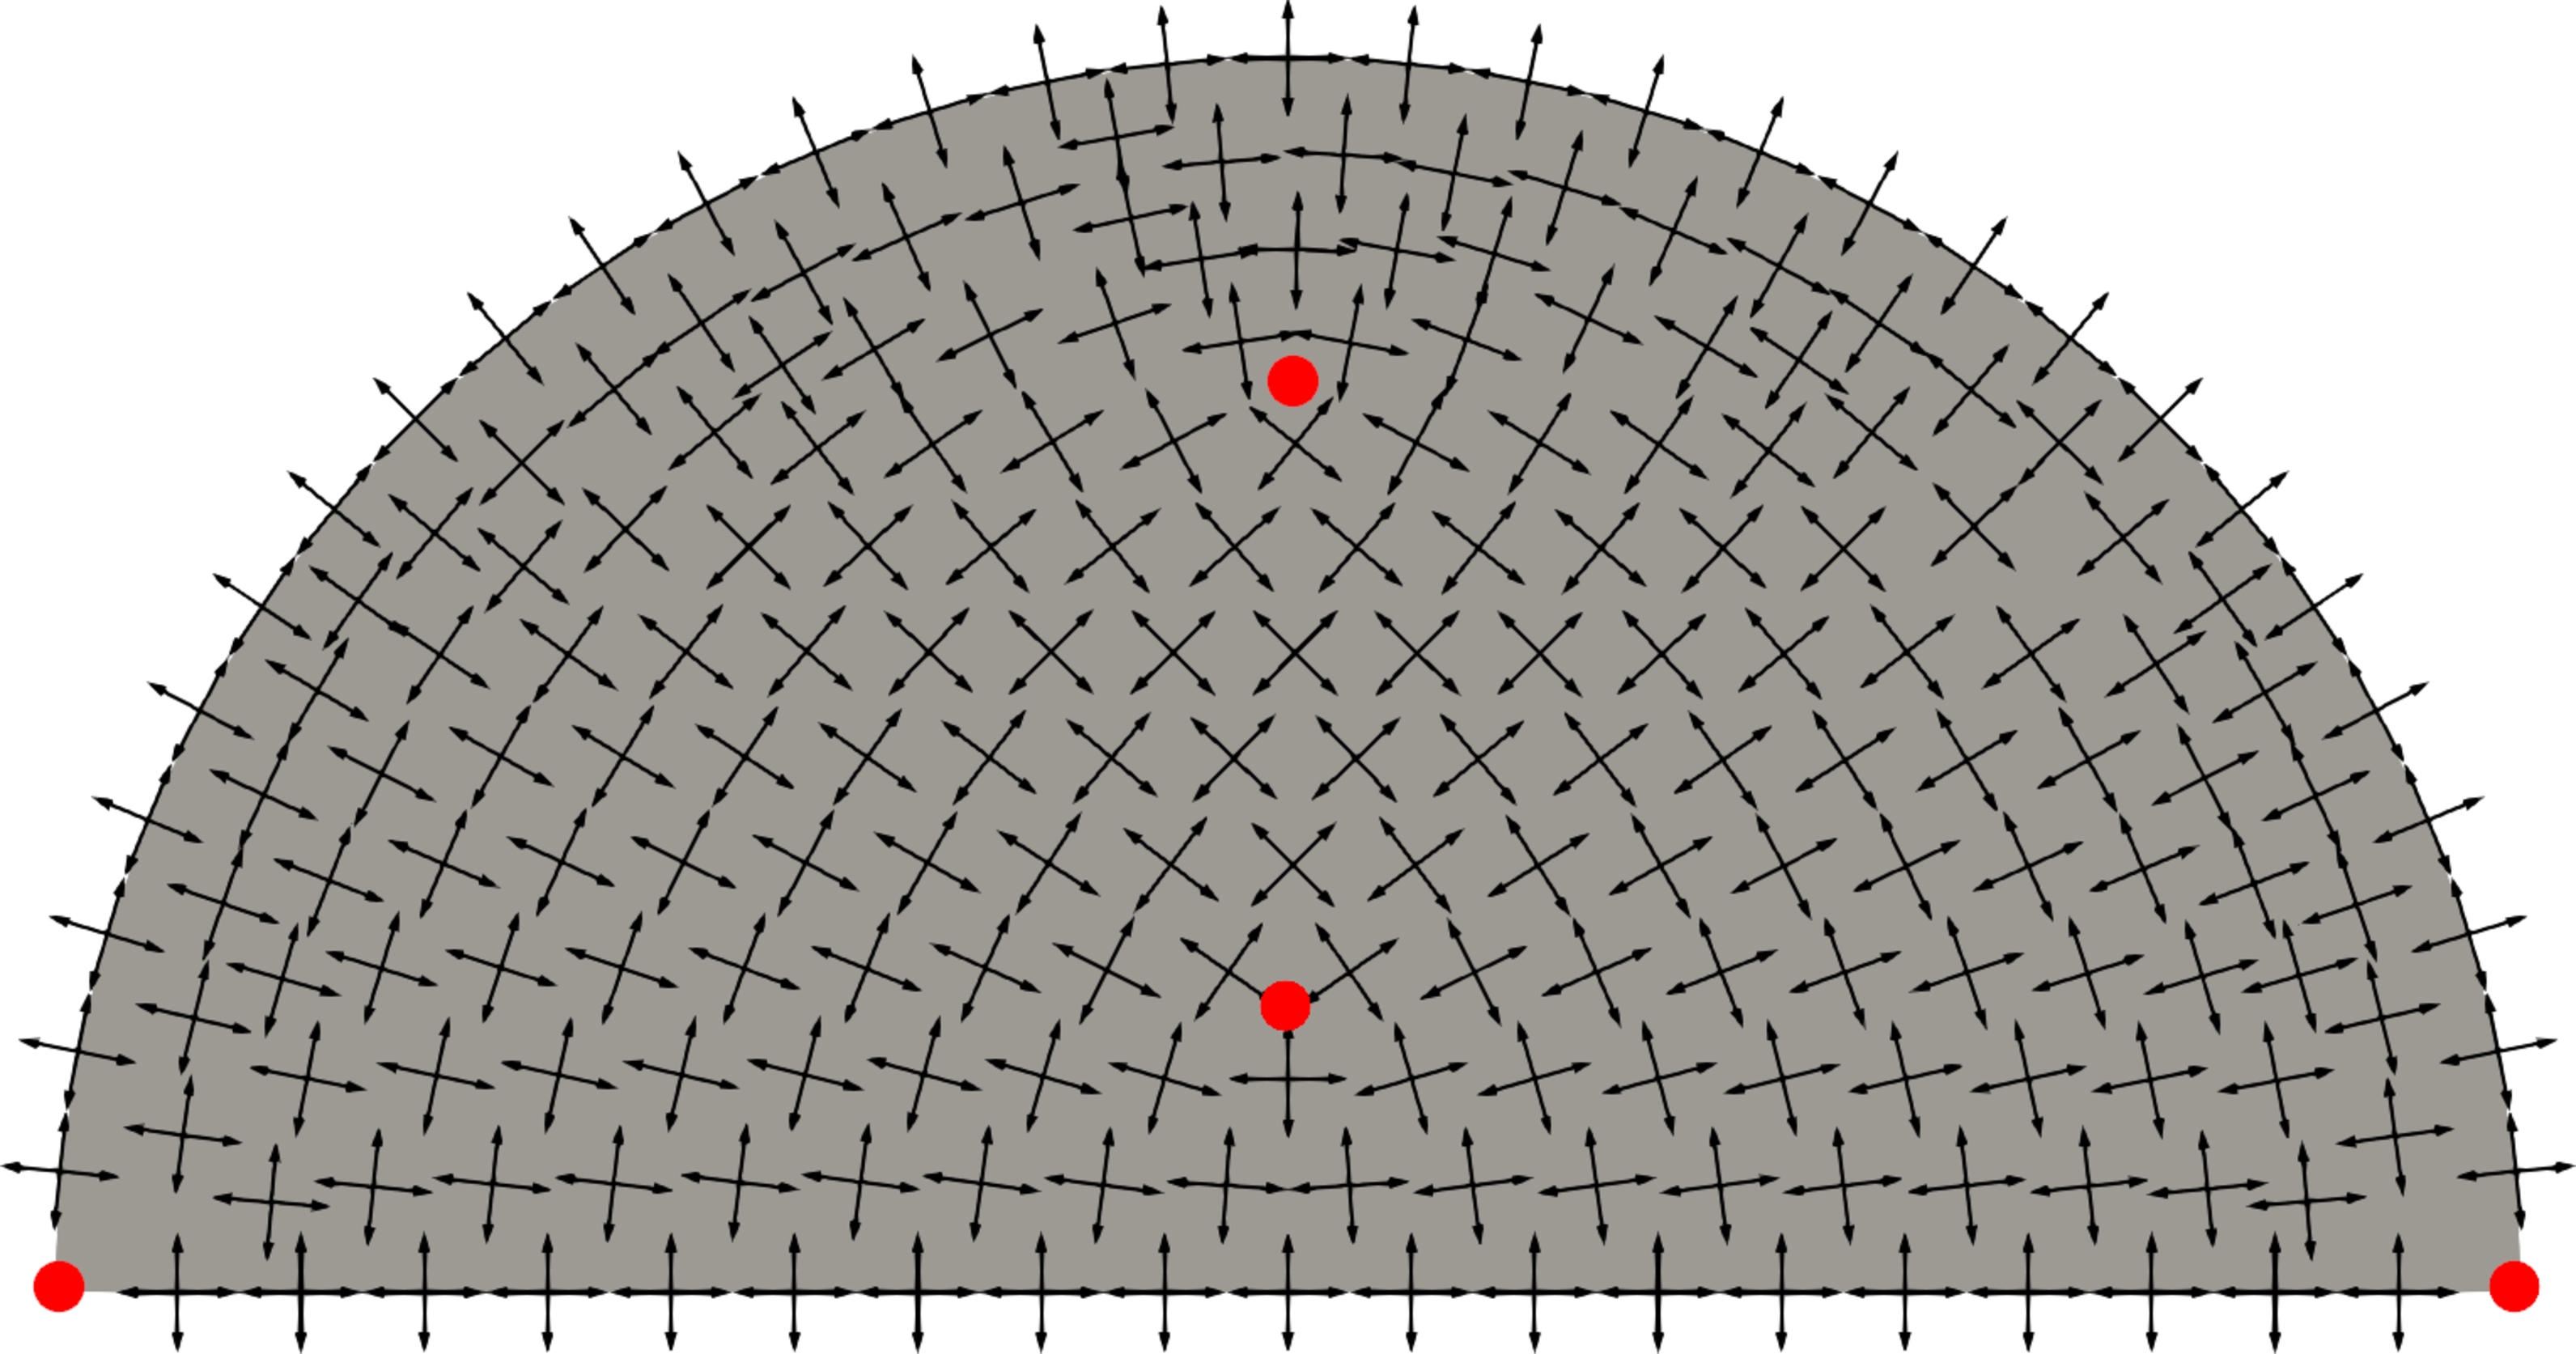
\includegraphics[scale=0.087]{images/demi_disc_align_first.pdf} \hspace{0.2cm}
        \footnotesize Cross-Field
        \end{column}
        \begin{column}{0.33\textwidth}
        \centering
        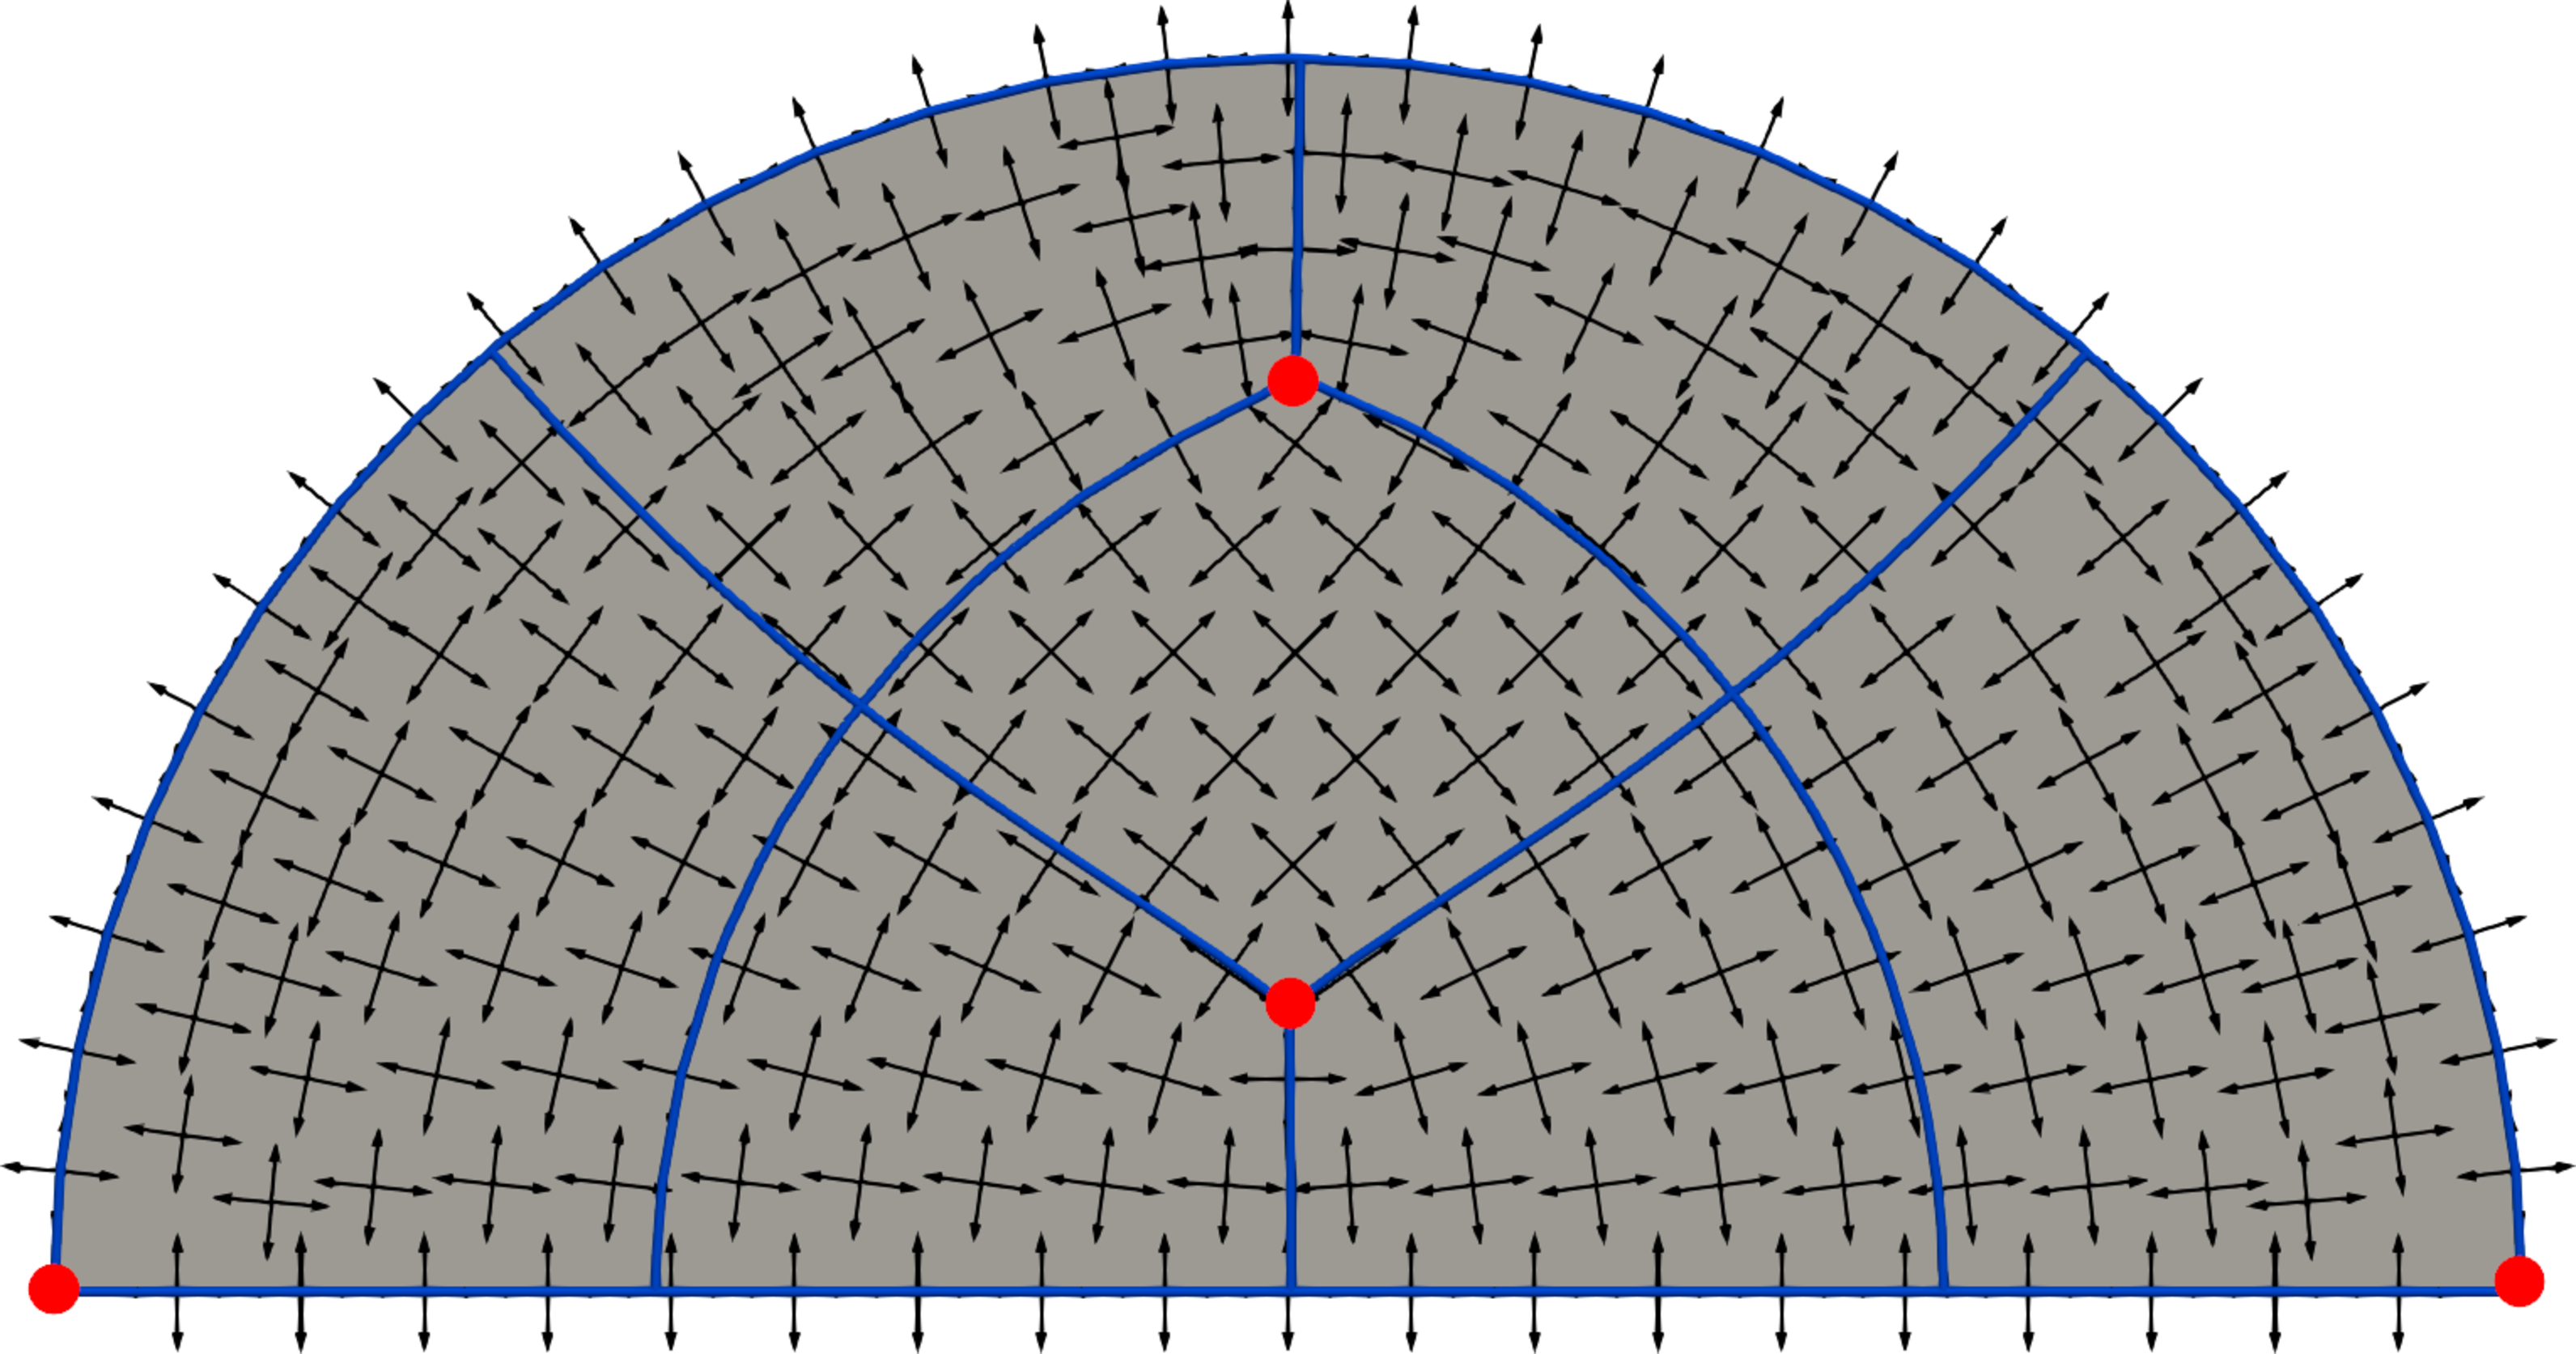
\includegraphics[scale=0.087]{images/demi_disc_align_second.pdf} \hspace{0.2cm}
        \footnotesize Partitioning
        \end{column}
        \begin{column}{0.33\textwidth}
        \centering
        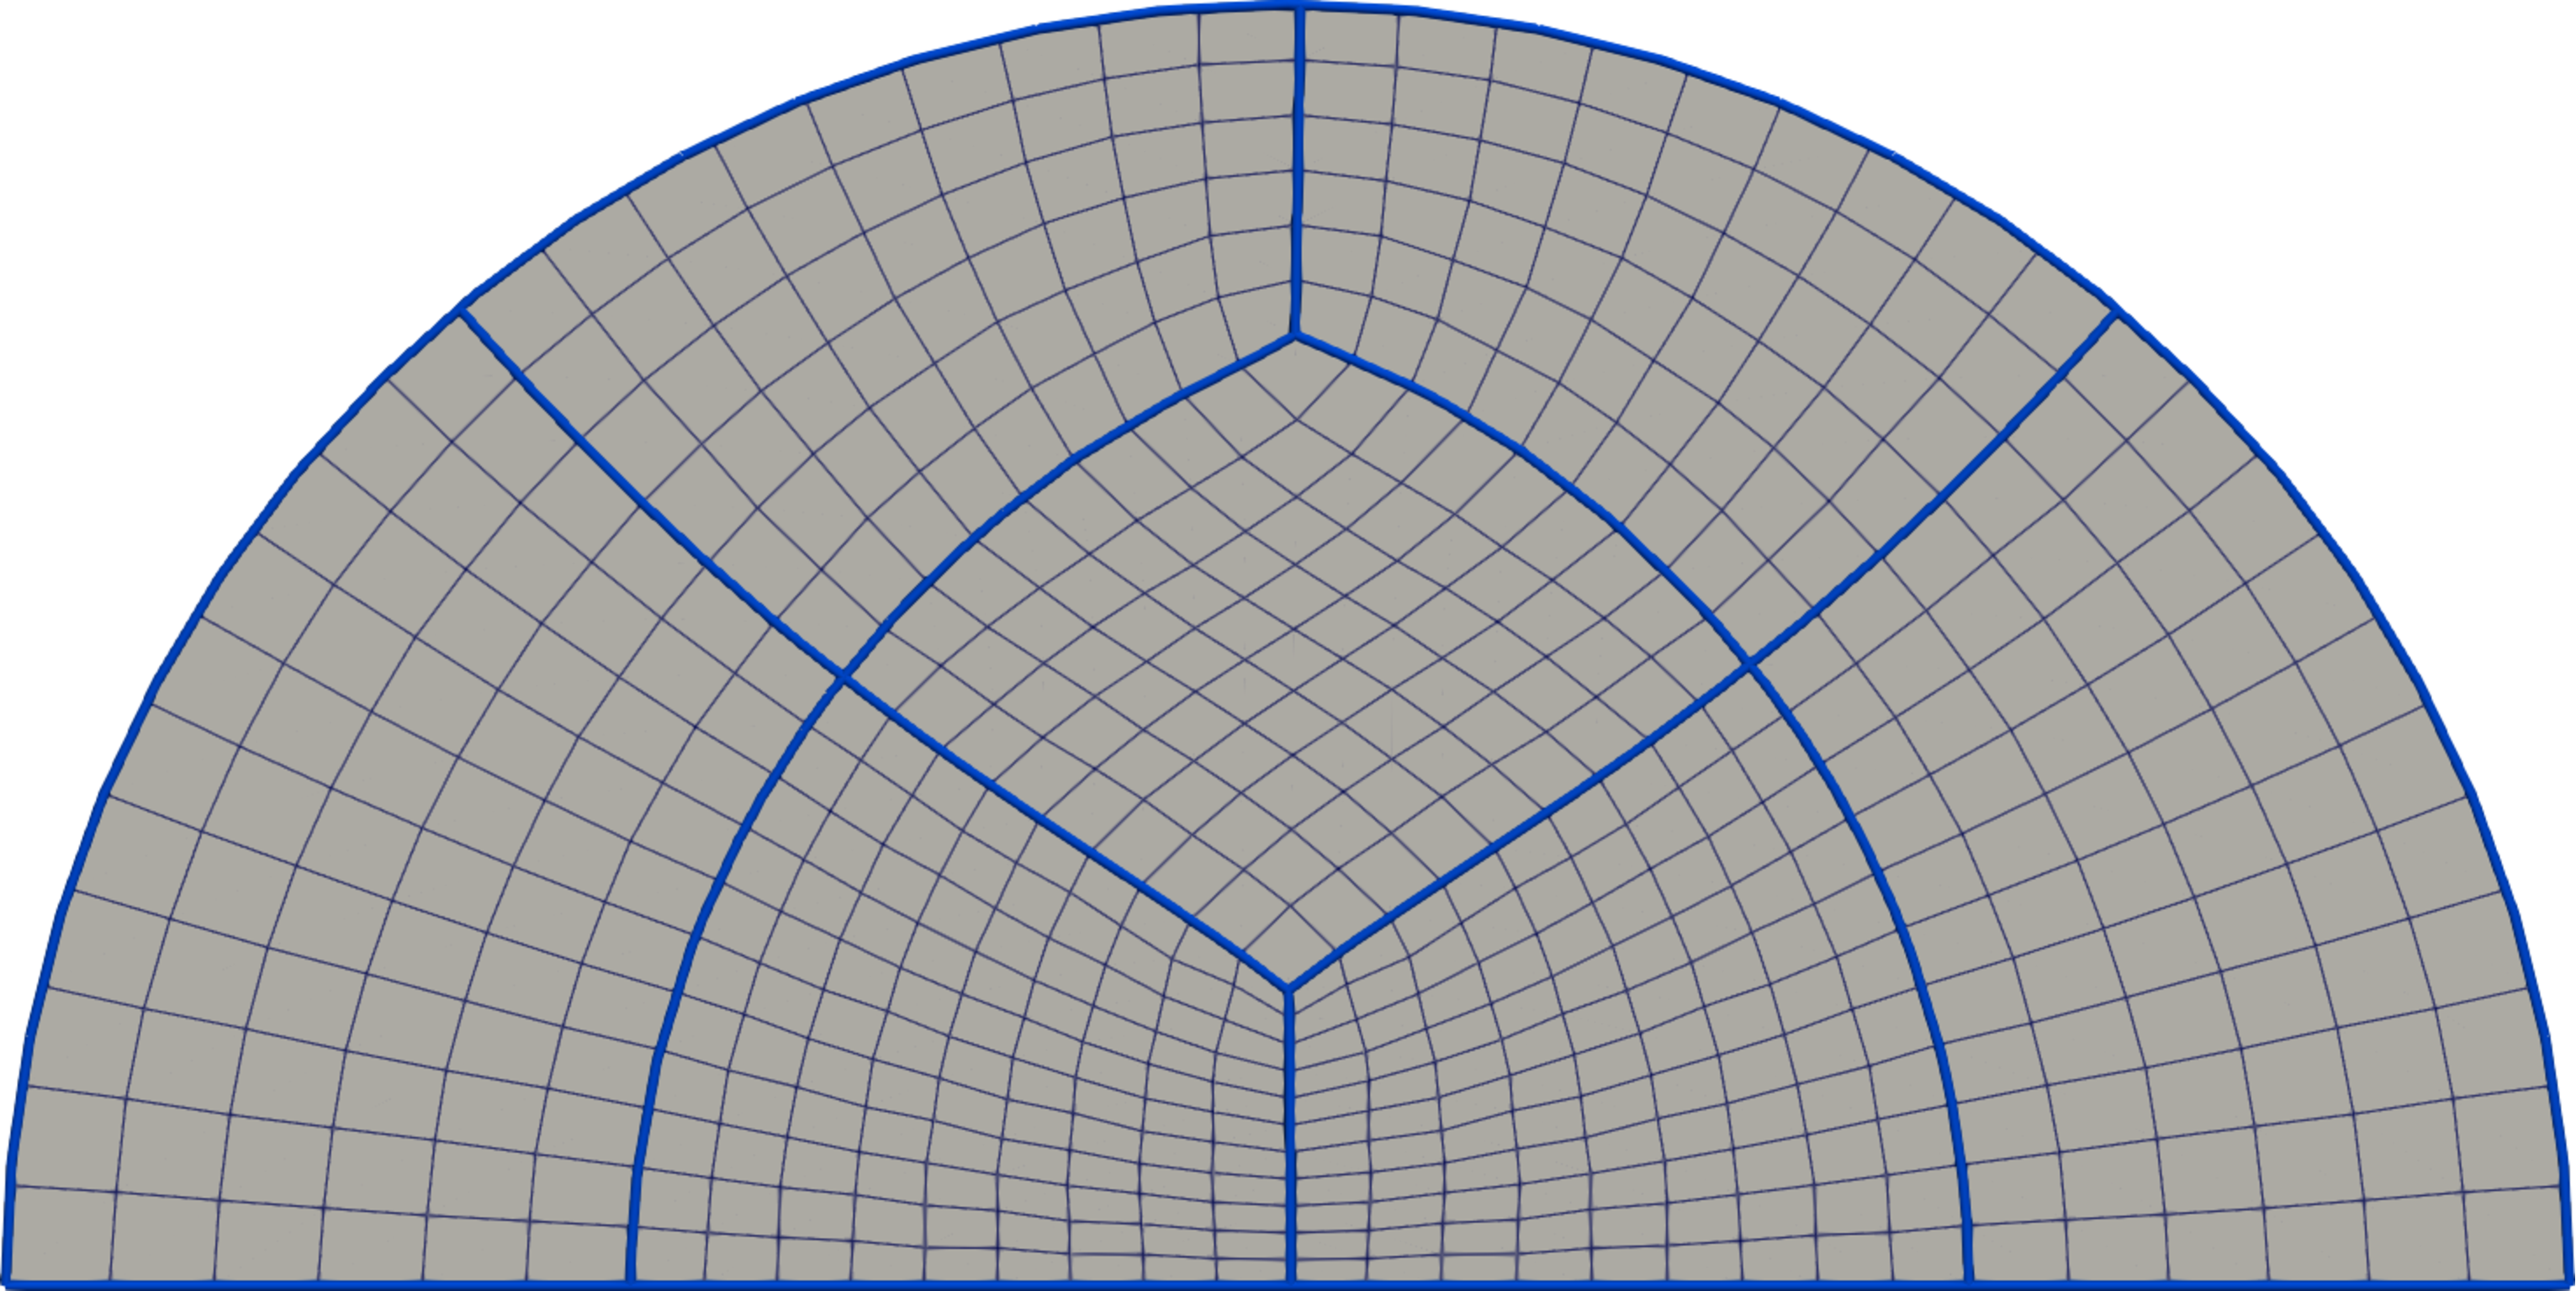
\includegraphics[scale=0.087]{images/demi_disc_align_third.pdf} \hspace{0.2cm}
        \footnotesize Meshing
        \end{column}
    \end{columns}
    \vspace{0.4cm}
        \begin{onerablock}[drop fuzzy shadow]{\small Theorem 1}
    \small
Let $\Omega$ be a bounded and closed domain in $\mathbb{R}^2$ with a piecewise smooth boundary and let $\bar{u}$ be an almost-$\mathcal{C}^1$ cross-field aligned with $\partial\Omega$ such that $0<Card(\mathcal{S}_{\bar{u}})<\infty$ and for all $p\in\Omega$, $id_{\bar{u}}(p)=k/4$ where $k\in\mathbb{Z}$ and $k\leq 1$. If the separatrices of $\bar{u}$ converge, then the resulting partition is a decomposition of $\Omega$ into four-sided regions.
    \end{onerablock}
\end{frame}



\begin{frame}{Alignment Process}
\small
\vspace{-0.3cm}
\begin{columns}
    \begin{column}{0.7\textwidth}

\onslide<2->{
\textbf{Idea}: Implementation of an alignment process by rotating the boundary crosses to align with the outward normal, ensuring a smooth global transformation of the field to avoid introducing singularities.%{\color{onera_gray}( Proposition)}
\\\vspace{0.12cm}
}

\onslide<3->{
\begin{onerablock}[drop fuzzy shadow]{\small Proposition}
    \small
    Let $\bar{u}$ be an almost-$\mathcal{C}^1$ cross-field on $\Omega$ and $\theta:\Omega \rightarrow \mathbb{R}$ a $\mathcal{C}^1$ function on $\Omega$, then $\bar{v}={\mathbf{R}(\theta)\bar{u}}$ is an almost-$\mathcal{C}^1$ cross-field and for all $p\in \Omega\backslash\partial\Omega,~id_{\bar{u}}(p)=id_{\mathbf{R}(\theta)\bar{u}}(p)$.
    \end{onerablock}
    %{\color{onera_gray}(Conservation of certain properties of $\bar{u}$)}\\\vspace{0.12cm}
    {\bf Diffusion of angular difference between $\bar{u}$ and $\bar{n}$:}
}

\vspace{0.1cm}

\onslide<3->{
%\vspace{0.4cm}
    \begin{equation*}
    \left\{
    \begin{array}{lcll}
    \Delta\phi &=& 0 &\mbox{ in }\Omega,\\[0.3cm]
    \phi(p) &=& \widehat{(\bar{n}(p); \bar{u}(p))}=\theta_{\bar{n}}(p)-\theta_{\bar{u}}(p)&\mbox{ on } \partial\Omega.
    \end{array}
    \right.
    \end{equation*}
    \footnotesize {{\color{onera_gray}(Multivalued angle, irregularity of $\phi$, boundary singularity introduction, boundary condition change.)}}\\\vspace{0.12cm}
}

\end{column}

\begin{column}{0.32\textwidth}
    \centering
    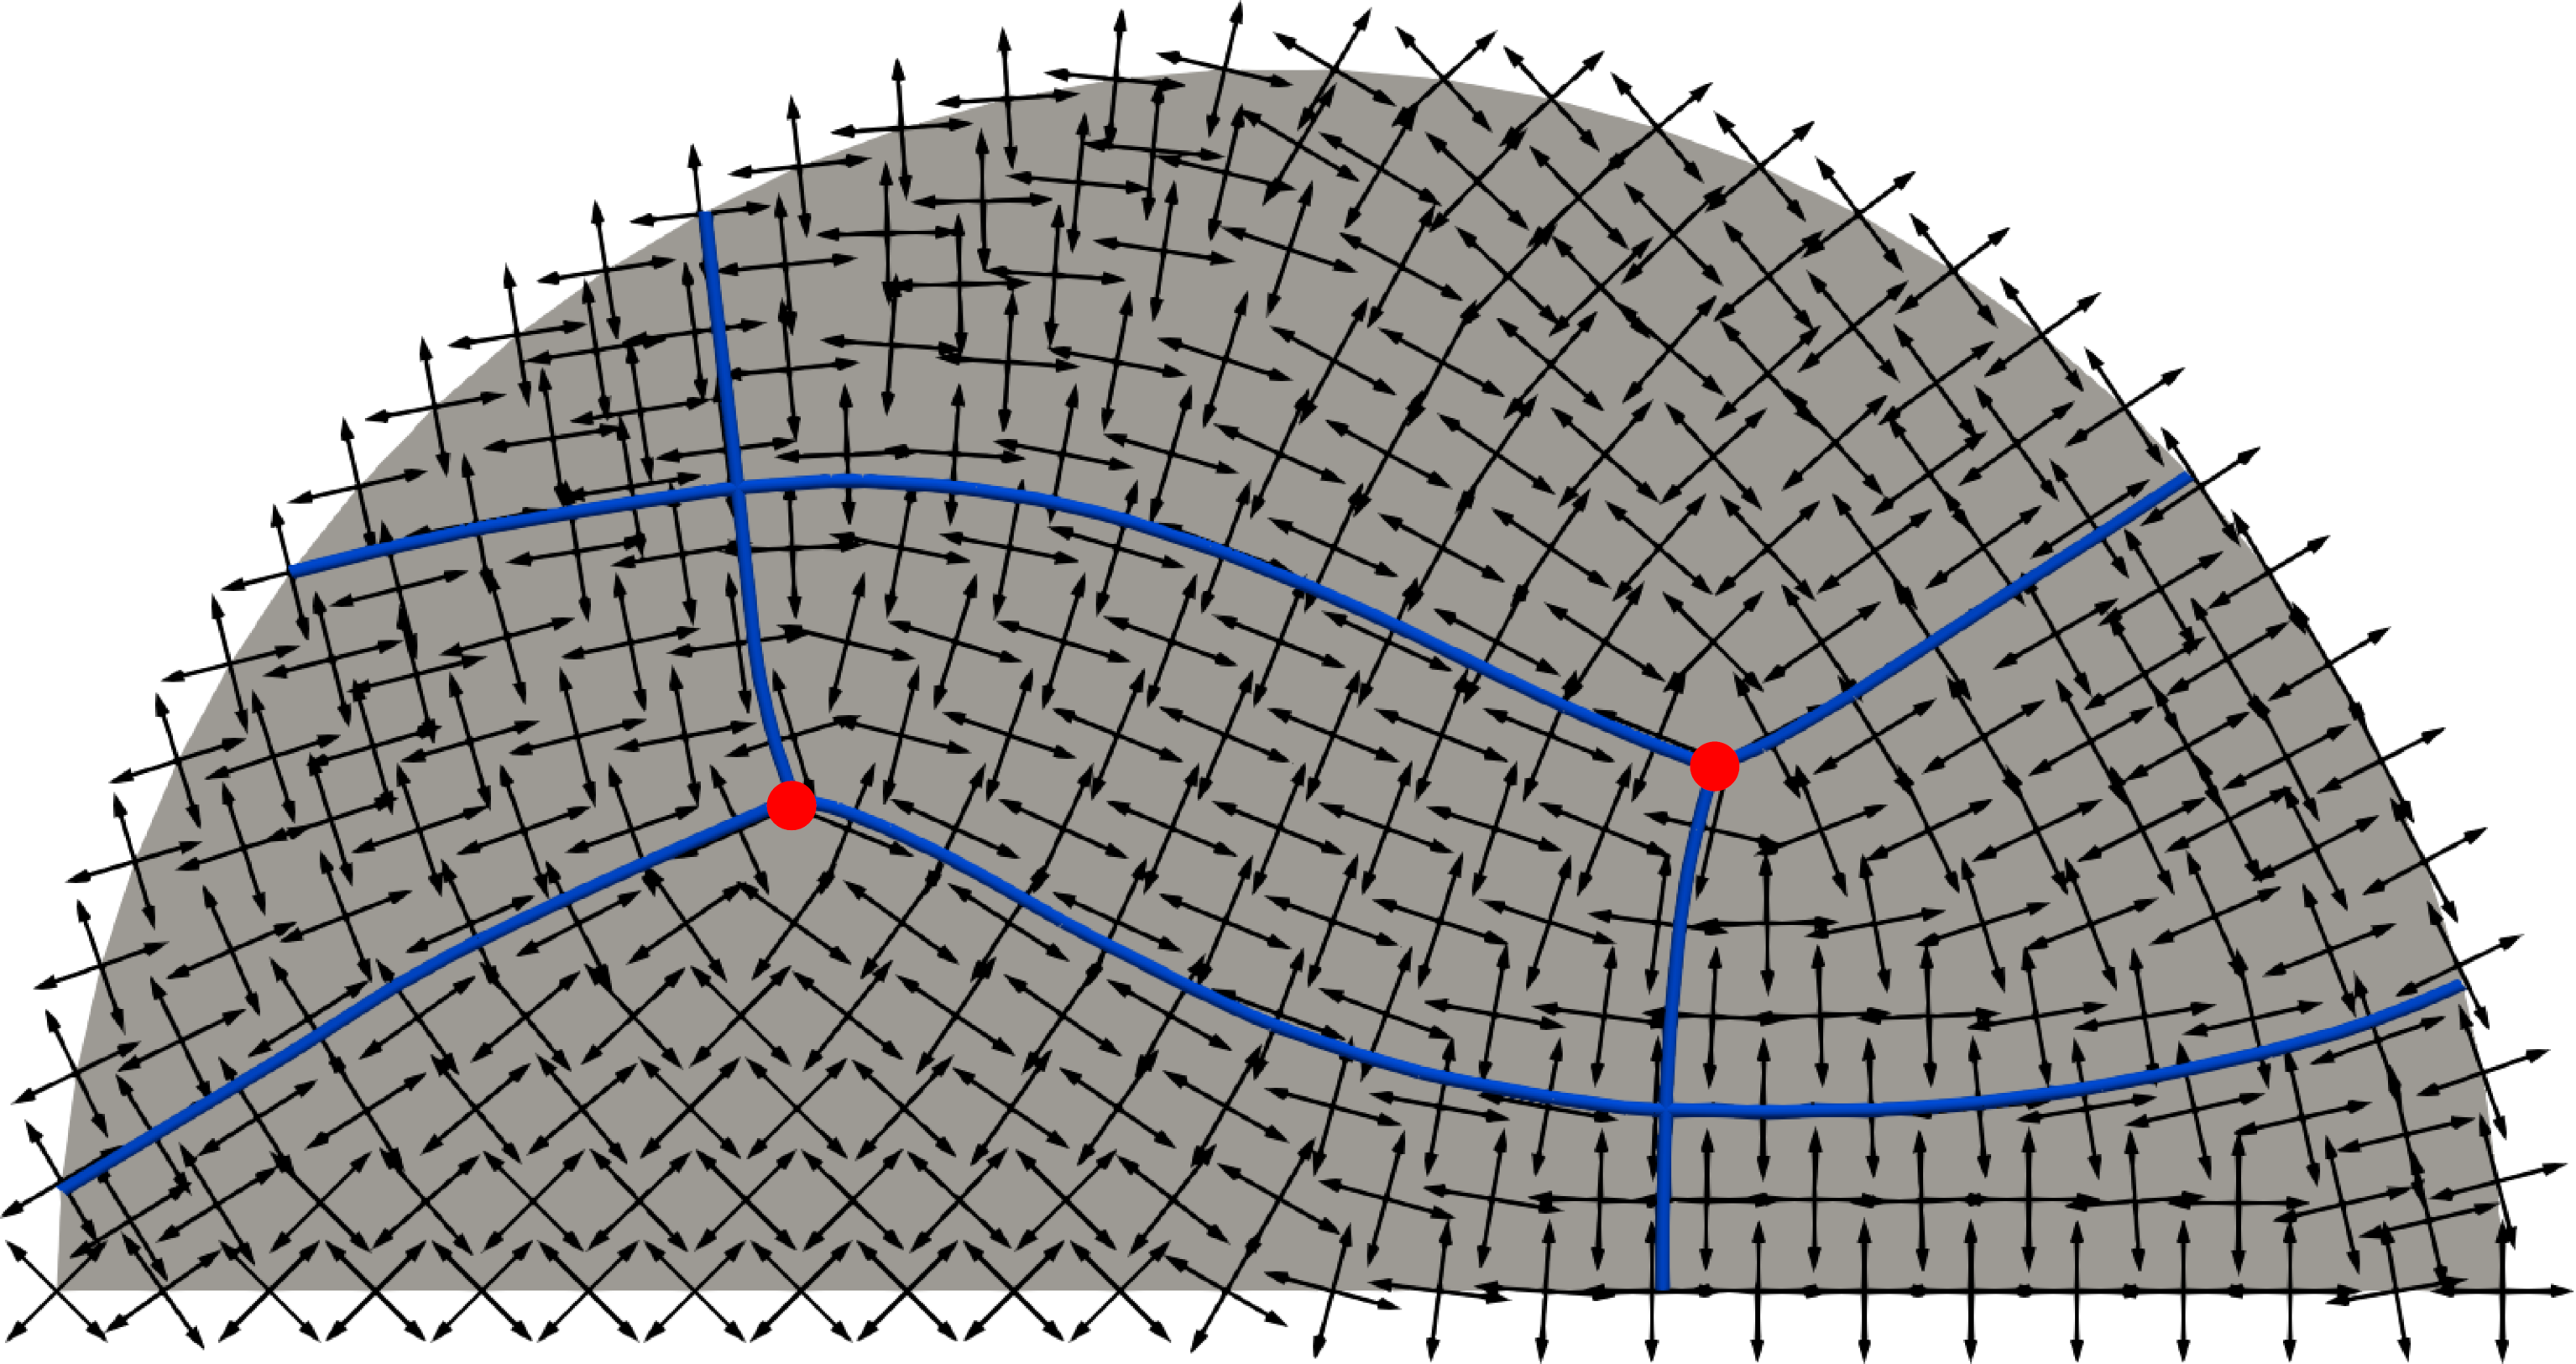
\includegraphics[scale=0.09]{images/mode_prop_stream_non_align_beam.pdf}
    \only<1>{
    \footnotesize {\color{onera_gray}(The boundary is not part of the separatrices. Cross-field not aligned with the domain boundary.)}
    }
\end{column}
\end{columns}
\end{frame}


\begin{frame}{Alignment Process}
\small
\vspace{-0.4cm}
Let \(\gamma\) be a parameterization on \([0, 1]\) of \(\partial\Omega\).\\\vspace{0.12cm}
\(\theta_{\bar{u}}^\gamma\) and \(\theta_{\bar{n}}^\gamma\) are continuous liftings of \(\theta_{\bar{u}}\) and \(\theta_{\bar{n}}\) along \(\gamma\).\\\vspace{0.12cm}
\textbf{Objective}: Smooth the angle while controlling the location of singularities due to the non-periodicity of the liftings. The alignment equation becomes:\\\vspace{0.12cm}

\begin{equation*}
\left\{
\begin{array}{lcll}
\Delta\phi &=& 0 &\mbox{ in } \Omega,\\[0.4cm]
\phi(\gamma(t)) &=& \theta_{\bar{n}}^\gamma(t) + \mathcal{I}(t) - \theta_{\bar{u}}^\gamma(t) & \mbox{ on } \gamma^{-1}(\partial\Omega \backslash (\mathcal{B} \cup \mathcal{S}_{\bar{n}} \cup \mathcal{S}_{\bar{u}})),
\end{array}
\right.
\end{equation*}

\begin{equation*}
\mathcal{I}(t) = \sum_{s \in \gamma^{-1}(\mathcal{B} \cup \mathcal{S}_{\bar{n}})} \left[\underbrace{\left(\pi - \widehat{\gamma(s)}\right)}_{\text{geodesic curvature}} - \underbrace{\left(\lim\limits_{r \rightarrow s^+}\theta^{\gamma}_{\bar{n}}(r) - \lim\limits_{r \rightarrow s^-}\theta^{\gamma}_{\bar{n}}(r)\right)}_{\text{jump of }\bar{n}} - \underbrace{2\pi I_{\gamma(s)}}_{\text{index of points in }\mathcal{B}\text{(the corners)}}\right] \mathbb{1}_{[0, t]}(s).
\end{equation*}

This ensures piecewise \(\mathcal{C}^1\) regularity where jumps are localized at points in the set \(\mathcal{B}\).

\end{frame}



\begin{frame}{Alignment Process}
\vspace{-0.2cm}
\small
By generalizing the Poincaré-Hopf theorem to the domain boundary, we obtain:
\begin{equation*}
\sum_{s\in \text{Int}(\Omega)} id_{\bar{v}}(s)+{\bf \color{red}\sum_{c\in \partial\Omega} id_{\bar{v}}(c)} = \chi(\Omega),
\label{poincareformula_3}
\end{equation*}
which provides a general constraint on the input cross field:
\begin{equation*}
\deg(\bar{u}, \partial\Omega) =\sum_{s\in \text{Int}(\Omega)} id_{\bar{u}}(s) = \sum_{s\in \text{Int}(\Omega)} id_{\bar{v}}(s) = \chi(\Omega)-\sum_{c\in \partial \Omega} id_{\bar{v}}(c).
\label{third_u_c}
\end{equation*}
\begin{onerablock}[drop fuzzy shadow]{Theorem 2}
Let $\bar{u}$ be a cross field such that for all $p\in\Omega\backslash\partial\Omega$, ${\bf id_{\bar{u}}(p)<=1/4}$. Given $\bar{u}$, a set $(c_i)_{i\in\{1,\dots,n_b\}}\subset\partial\Omega$ of distinct points such that:
$
{\bf \deg(\bar{u}, \partial\Omega) = \chi(\Omega)-\sum_{i=1}^{n_b} id_{\bar{u}}(c_i),}
$
there exists a cross field $\bar{v}$ aligned with the boundary of $\Omega$ that satisfies Theorem 1.
\end{onerablock}
\vspace{0.1cm}
{\bf Example:} Cross field constructed from the eigenmode of the Laplacian on the half-disc.
\end{frame}



\begin{frame}%{\fontsize{12}{12}\selectfont Examples}
\vspace{-0.28cm}
\begin{columns}
\begin{column}{0.4\textwidth}
    \centering
    \scriptsize
    $\chi(\Omega)=1$\\\vspace{0.1cm}
    $\deg(\bar{u}, \partial\Omega) = 1/4+1/4$\\\vspace{0.1cm}
    $\sum_{i=1}^{2} id_{\bar{u}}(c_i)=1/4+1/4$\\\vspace{0.1cm}
    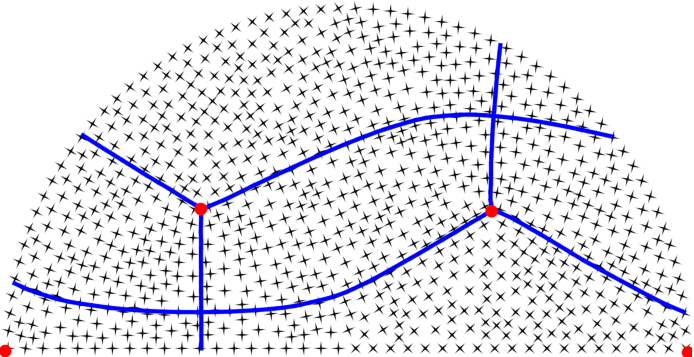
\includegraphics[scale=0.32]{images/demiDiscValPropNonAligne.pdf}\\\vspace{0.1cm}
    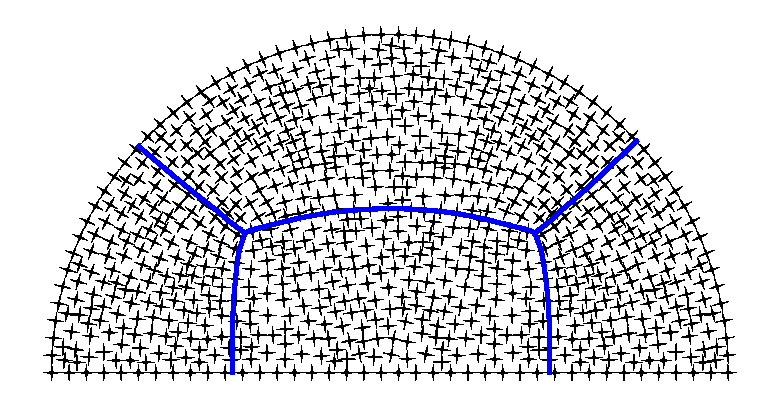
\includegraphics[scale=0.32]{images/demiDiscValPropAligne.eps}\\\vspace{0.1cm}
    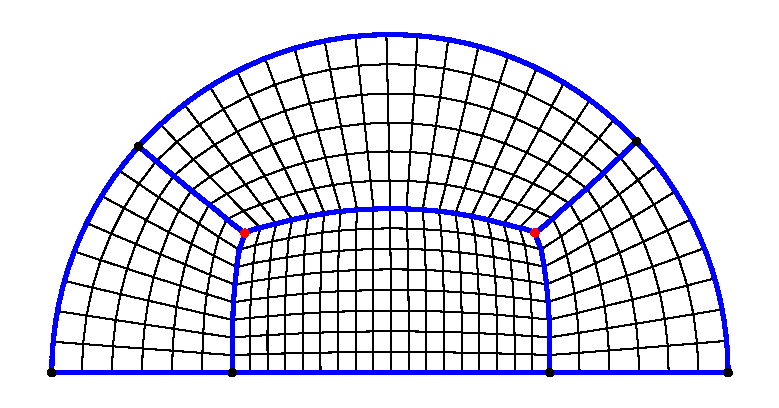
\includegraphics[scale=0.32]{images/mailDemiDisc.eps}\\
    \scriptsize {\color{onera_gray}(Eigenmode)}
\end{column}
\pause
\begin{column}{0.4\textwidth}
    \centering
    \scriptsize
    $\chi(\Omega)=1$\\\vspace{0.1cm}
    $\deg(\bar{u}, \partial\Omega) = 1/4+1/4$\\\vspace{0.1cm}
    $\sum_{i=1}^{2} id_{\bar{u}}(c_i)=1/4+1/4$\\\vspace{0.1cm}
    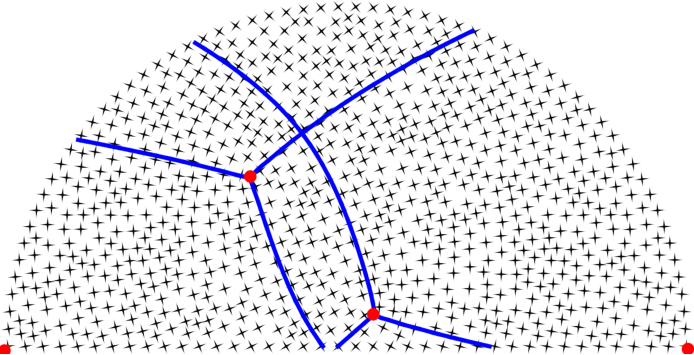
\includegraphics[scale=0.32]{images/demiDiscGinzNonAligne.pdf}\\\vspace{0.1cm}
    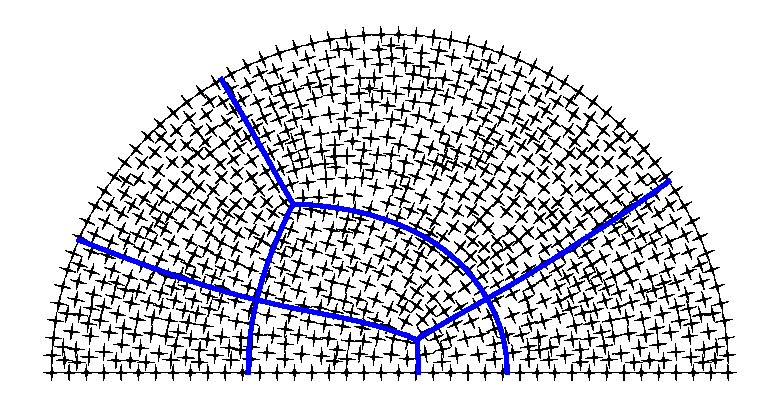
\includegraphics[scale=0.32]{images/demiDiscGinzAligne.eps}\\\vspace{0.1cm}
    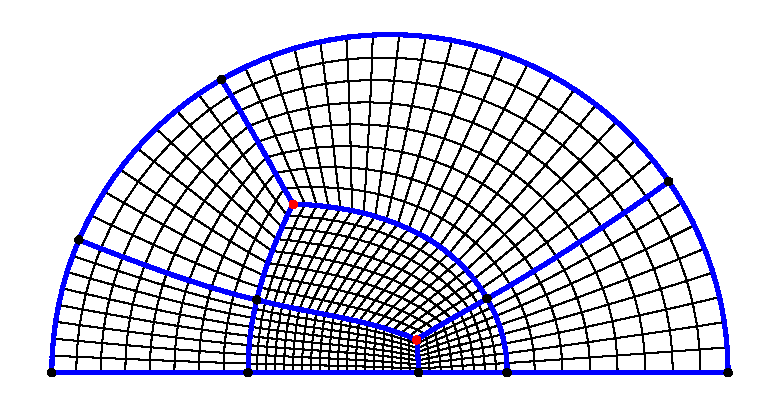
\includegraphics[scale=0.32]{images/demiDiscMail.eps.eps}\\
    \scriptsize {\color{onera_gray}(Analytical field)}
\end{column}
\pause
\begin{column}{0.4\textwidth}
    \centering
    \scriptsize
    $\chi(\Omega)=1$\\\vspace{0.1cm}
    $\deg(\bar{u}, \partial\Omega) = 1/4+1/4+1/4$\\\vspace{0.1cm}
    $\sum_{i=1}^{3} id_{\bar{u}}(c_i)=1/4+1/4-1/4$\\\vspace{0.1cm}
    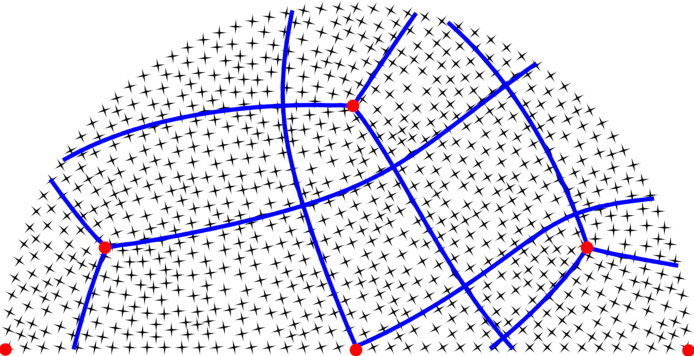
\includegraphics[scale=0.32]{images/demiDiscTroisPointNonAligne.pdf}\\\vspace{0.1cm}
    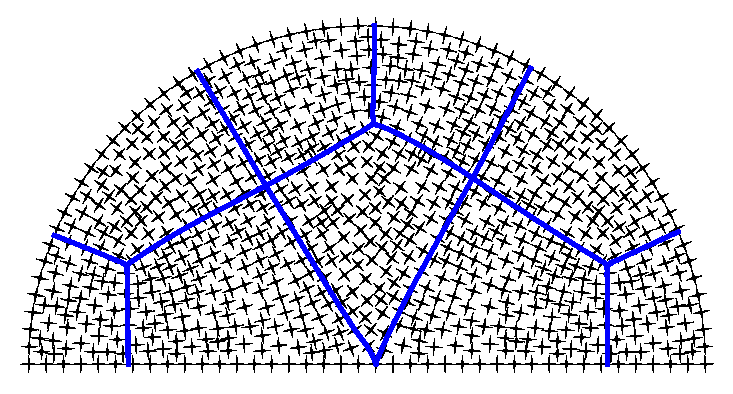
\includegraphics[scale=0.32]{images/demiDIscTroisPointAligne.eps}\\\vspace{0.1cm}
    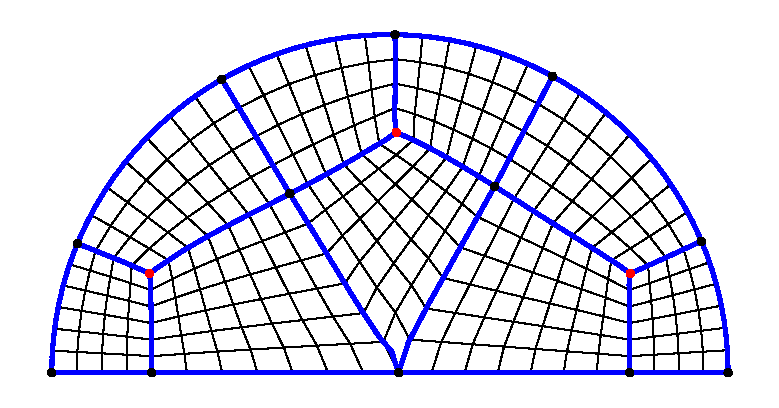
\includegraphics[scale=0.32]{images/mesh_quad_3.eps}\\
    \scriptsize {\color{onera_gray}(Bonus: boundary singular points, corner view)}
\end{column}
\end{columns}
\end{frame}




\begin{frame}{Outline}
    %\tableofcontents
    \vspace{-0.4cm}
    \begin{enumerate}
        \item \color{onera} Context and Objectives \\\vspace{0.26cm}
        \item Formalizing the Partitioning Process %{\color{onera_gray}(new perspective, field alignment on the boundary, ...)}
        \vspace{0.26cm}
        \begin{itemize}
            \item Handling Arbitrary Cross-Fields\\\vspace{0.18cm}
            \item Alignment Process\\\vspace{0.18cm}
            \item Non-Simply Connected Domains\\\vspace{0.18cm}
            %\item Discussions (some theoretical results)\\\vspace{0.18cm}
            %\item Examples%\\\vspace{0.2cm}
        \end{itemize}
        %\item Handling Boundary Singularities {\color{onera_gray}(considering boundary conditions, ...)}\\\vspace{0.5cm}
        %\item Handling Arbitrary Cross-Fields {\color{onera_gray}(domains with holes, multi-material, ...)}\\\vspace{0.34cm}
        \item Discretization and Extension to Non-Planar Surface Manifolds %{\color{onera_gray}(considering curvature, generalization, ...)}\\
        \vspace{0.26cm}
        \begin{itemize}
            \item Partitioning Process\\\vspace{0.18cm}
            \item Convergence Analysis\\\vspace{0.18cm}
            %\item Examples%\\\vspace{0.2cm}
        \end{itemize}
        \item Conclusion and Perspectives
    \end{enumerate}
\end{frame}



\begin{frame}{Non-simply connected domains}
\small
\vspace{-0.5cm}
\begin{columns}
\begin{column}{0.85\textwidth}
%\vspace{0.08cm}
{\color{onera_gray}(Domain consisting of a single component with multiple boundaries, which cannot be continuously reduced to a point, domains with holes)}\\\vspace{0.08cm}
%\textbf{Application to a domain with a hole:}
Let $\partial\Omega=\cup_i\Gamma_i$, with $(b_j^i)_{i,j}$ the boundary singular points.\\\vspace{0.12cm}
%\vspace{0.08cm}
The constraint on $\bar{u}$ becomes:
    $\deg(\bar{u}, \partial\Omega)=\sum_i \deg(\bar{u},\Gamma_i)=\chi(\Omega)-\sum_i\sum_j id_{\bar{u}}(b_j^i).$\\\vspace{0.12cm}
%\vspace{-0.1cm}
%\\[-0.1cm]
\textbf{Example:} Square with a hole, $\chi(\Omega)=0, \sum_i\sum_j id_{\bar{u}}(b_j^i)=1/4+1/4+1/4+1/4$\\\vspace{0.12cm}
We can take $\bar{u}$ such that $\deg(\bar{u}, \partial\Omega)=-1/4-1/4-1/4-1/4$\\\vspace{0.12cm}
{\color{onera_gray} Alignment process failure. Irregularity of the field due to the non-periodicity of the difference of crosses on the boundaries (see figure).}\\\vspace{0.08cm}
\end{column}
\begin{column}{0.18\textwidth}
\centering
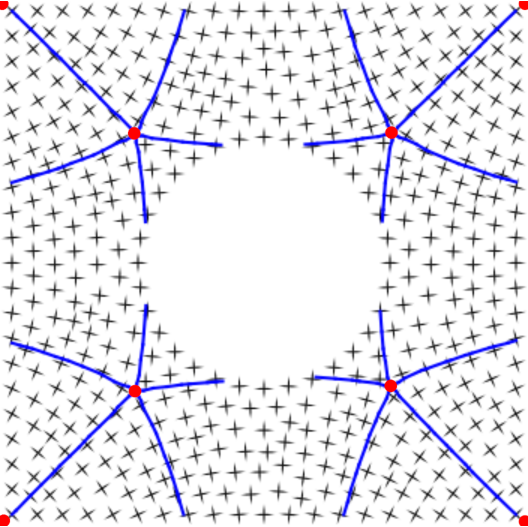
\includegraphics[scale=0.32]{images/carreDiscVide_stream_non_align_beam.pdf}
\end{column}
\end{columns}
\vspace{0.05cm}
\centering
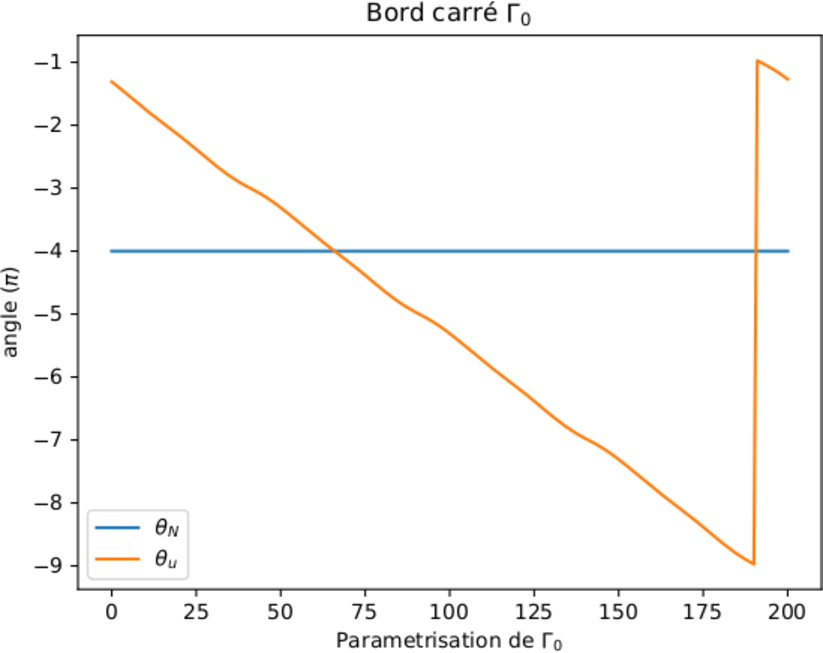
\includegraphics[width=6cm, height=2.45cm]{images/courbe_1.pdf}\hspace{0.6cm}
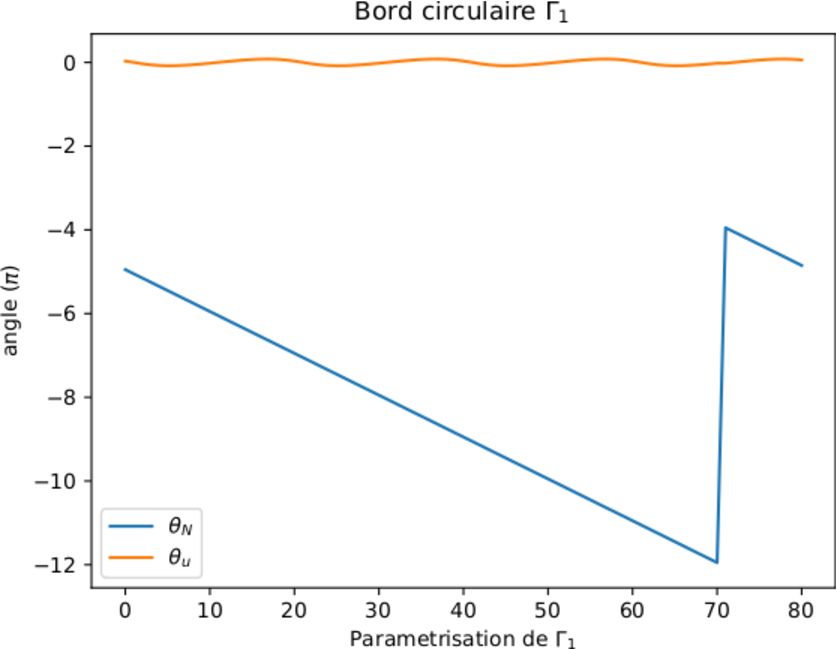
\includegraphics[width=6cm, height=2.45cm]{images/courbe_0.pdf}
\end{frame}





\begin{frame}{Non-simply connected domains}{}
\small
For this to work, the cross field $\bar{u}$ must satisfy:\\\vspace{0.2cm}
\begin{equation*}
\left\{
\begin{array}{lcll}
   \deg(\bar{u},\Gamma_0)&=&2\pi-2\pi\sum_j id_{\bar{u}}(b_j^0)&\mbox{ on }\Gamma_0,\\[0.3cm]
   \deg(\bar{u}, \Gamma_i)&=&-2\pi-2\pi\sum_j id_{\bar{u}}(b_j^i)&\mbox{ on }\Gamma_i~~~\forall~i.
\end{array}
\right.
\end{equation*}
\\\vspace{0.2cm}
{\color{onera_gray} This is the same condition as before but imposed on each boundary.}\\\vspace{0.12cm}
We retrieve this condition using the correction field satisfying the following weak equation:
\vspace{0.12cm}
\begin{equation*}
\left\{
\begin{array}{lcll}
    \triangle h &= &0 &\mbox{ in }\Omega,\\[0.25cm]
    \displaystyle\frac{1}{2\pi}\int_{\Gamma_0}\theta_h &=& \deg(\bar{u}, \Gamma_0)-1+\sum_j id_{\bar{u}}(b_j^0))&\mbox{ on } \Gamma_0,\\[0.25cm]
    \displaystyle\frac{1}{2\pi}\int_{\Gamma_i}\theta_h& =& \deg(\bar{u}, \Gamma_i)-1-\sum_j id_{\bar{u}}(b_j^i),&\mbox{ on }\Gamma_i~~~\forall~i.
\end{array}
\right.
\end{equation*}

\end{frame}


\begin{frame}{Non-simply connected domains}

\vspace{-0.3cm}
\small
\begin{columns}
\begin{column}{0.68\textwidth}
The alignment equation then takes the following form: {\color{onera_gray} (where the correction field is included in the boundary condition.)}
\begin{equation*}
\left\{
\begin{array}{lcll}
    \triangle\phi& =& 0& \mbox{ in }\Omega,\\[0.25cm]
    \phi &=& \theta_{\bar{n}_{|\Gamma_i}}-\theta_{\bar{u}_{|\Gamma_i}}-\theta_{h_{|\Gamma_i}}& \mbox{ on }\Gamma_i, \forall i.
\end{array}
\right.
\end{equation*}
Final cross field {\color{onera_gray} (obtained via a double rotation, correction field, aligned field)}
\begin{equation*}
\bar{v}=R(\phi)R(\theta_h)\bar{u}.
\end{equation*}
\textbf{Example:} Application to a square with a hole.\\\vspace{0.2cm}
\begin{onerablock}[drop fuzzy shadow]{
\small Theorem 3}
Given $\bar{u}$ with a set $(c_i)_{i\in\{1,\dots,n_b\}}\subset\partial\Omega$ of distinct points such that:
$
{\bf deg(\bar{u}, \partial\Omega) = \chi(\Omega)-\sum_{i=1}^{n_b} id_{\bar{u}}(c_i),}
$
the cross field $\bar{v}=R(\phi)R(\theta_h)\bar{u}$ satisfies Theorem 1.
\end{onerablock}
\end{column}
\begin{column}{0.32\textwidth}
\centering
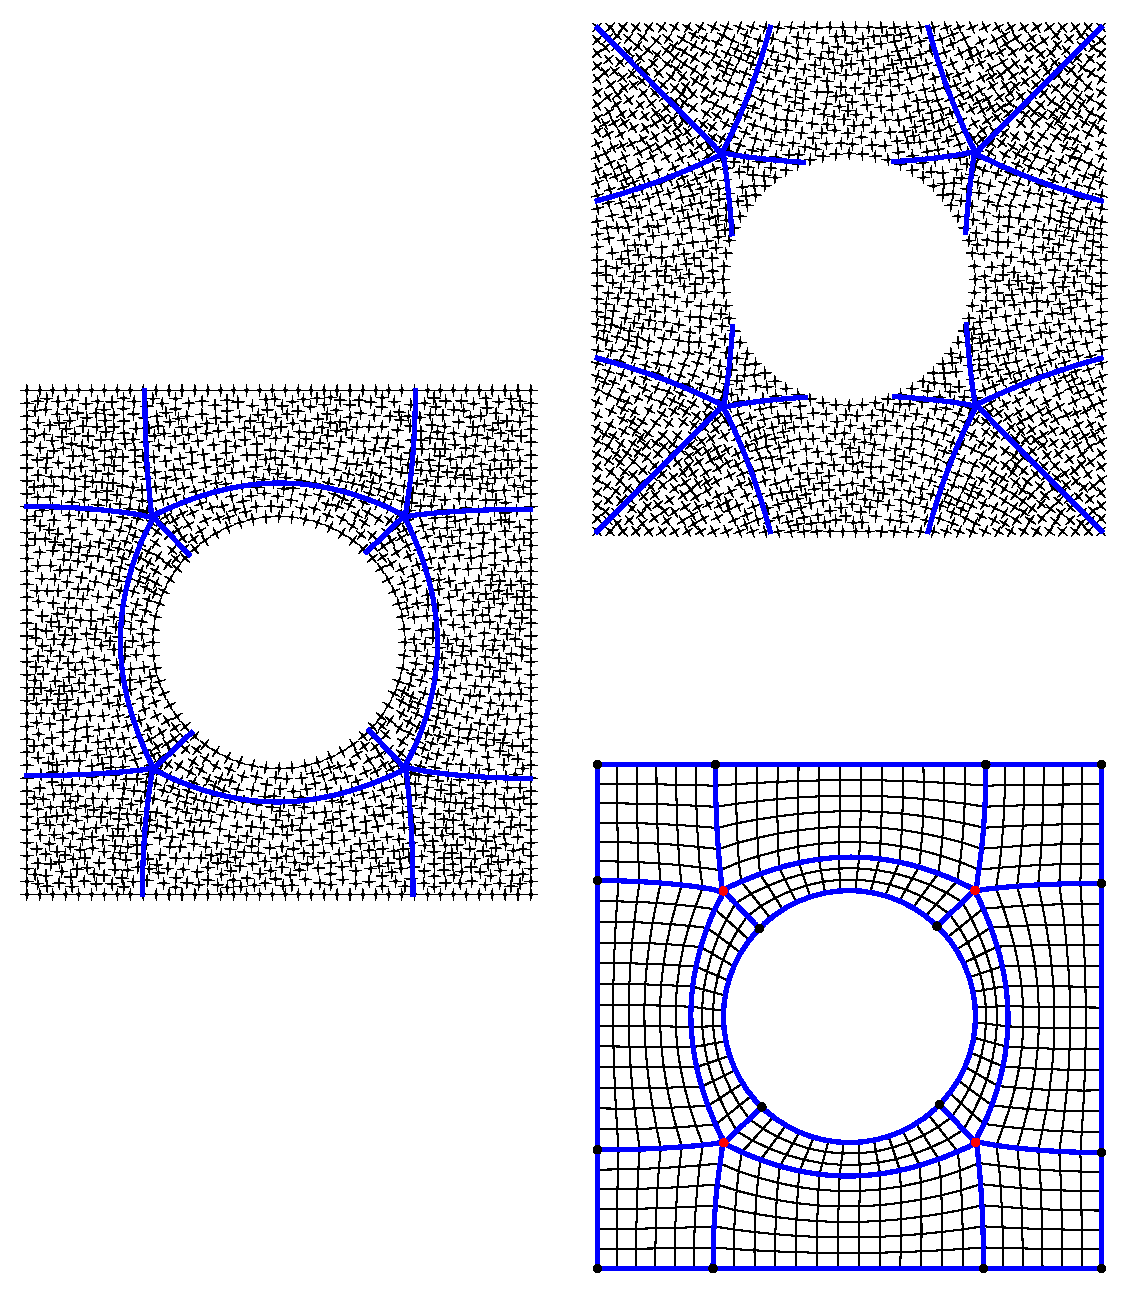
\includegraphics[scale=0.27]{images/image.eps}
\end{column}
\end{columns}
\end{frame}


\begin{frame}{Examples}%{ Some domains with holes and a domain with multiple connected components}
\vspace{-0.25cm}
\begin{columns}
\begin{column}{0.34\textwidth}
    \centering
    \onslide<1->{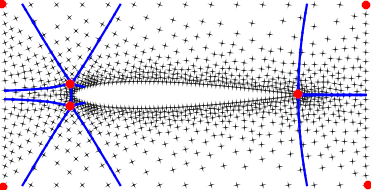
\includegraphics[scale=0.35]{images/1_beam.png}\\\vspace{0.1cm}
    \scriptsize
    $\chi(\Omega)=0$; $deg(\bar{u}, \partial\Omega) = -1/4-1/4$\\\vspace{0.1cm}
    $\sum_{i=1}^{5} id_{\bar{u}}(c_i)=1/4+1/4+1/4+1/4-1/2$\\\vspace{0.1cm}\vspace{0.6cm}
    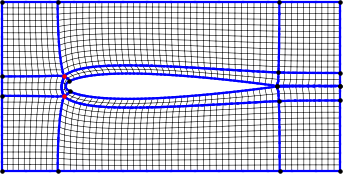
\includegraphics[scale=0.35]{images/2.png}}
\end{column}
\begin{column}{0.34\textwidth}
    \centering
    \onslide<2->{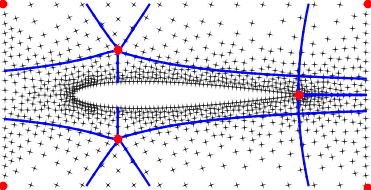
\includegraphics[scale=0.35]{images/3_beam.png}\\\vspace{0.1cm}
    \scriptsize
    $\chi(\Omega)=0$; $deg(\bar{u}, \partial\Omega) = -1/4-1/4$\\\vspace{0.1cm}
    $\sum_{i=1}^{5} id_{\bar{u}}(c_i)=1/4+1/4+1/4+1/4-1/2$\\\vspace{0.1cm}\vspace{0.6cm}
    \includegraphics[scale=0.35]{images/4.png}}
\end{column}
\begin{column}{0.34\textwidth}
    \centering
    %\includegraphics[scale=0.31]{images/mesh_quad_6.pdf}\\\vspace{-0.2cm}
    %\scriptsize\color{onera_gray}{ Multi-material }
    \onslide<3->{\includegraphics[scale=0.35]{images/mailNautilus.eps}\\\vspace{0.1cm}
    \scriptsize
    $\chi(\Omega)=0$\\\vspace{0.1cm}
    $deg(\bar{u}, \partial\Omega) = 1/4+1/4+1/4+1/4-1/4-1/4-1/4-1/4$\\\vspace{0.1cm}
    $\sum_{i=1}^{2} id_{\bar{u}}(c_i)=1/4-1/4$\\\vspace{0.2cm}
    %\includegraphics[scale=0.35]{images/mailNautilus.eps}\\\vspace{-0.1cm}
    \scriptsize\color{onera_gray}{ Nautilus}}
\end{column}
\end{columns}
\end{frame}



% \begin{frame}{Outline}
%     %\tableofcontents
%     \vspace{-0.4cm}
%     \begin{enumerate}
%         \item \color{onera} Context and Objectives \\\vspace{0.26cm}
%         \item Formalizing the Partitioning Process %{\color{onera_gray}(new perspective, field alignment on the boundary, ...)}
%         \vspace{0.26cm}
%         \begin{itemize}
%             \item Handling Arbitrary Cross-Fields\\\vspace{0.18cm}
%             \item Alignment Process\\\vspace{0.18cm}
%             \item Non-Simply Connected Domains\\\vspace{0.18cm}
%             \item Discussions (some theoretical results)\\\vspace{0.18cm}
%             %\item Examples%\\\vspace{0.2cm}
%         \end{itemize}
%         %\item Handling Boundary Singularities {\color{onera_gray}(considering boundary conditions, ...)}\\\vspace{0.5cm}
%         %\item Handling Arbitrary Cross-Fields {\color{onera_gray}(domains with holes, multi-material, ...)}\\\vspace{0.34cm}
%         \item Discretization and Extension to Non-Planar Surface Manifolds %{\color{onera_gray}(considering curvature, generalization, ...)}\\
%         \vspace{0.26cm}
%         \begin{itemize}
%             \item Partitioning Process\\\vspace{0.18cm}
%             \item Convergence Analysis\\\vspace{0.18cm}
%             %\item Examples%\\\vspace{0.2cm}
%         \end{itemize}
%         \item Conclusion and Perspectives
%     \end{enumerate}
% \end{frame}


% \begin{frame}{Discussions}{On the initialization of separatrices}

% \vspace{-0.3cm}
% \small
% \only<1>{
% \begin{columns}
% \begin{column}{0.7\textwidth}

% The initialization of separatrices presents a well-known problem in ODEs, which is how to \textbf{trace a field line from a given singular point?}\\\vspace{0.15cm}
% We propose the following result:\\\vspace{0.15cm}
% \begin{onerablock}[drop fuzzy shadow]{\small Proposition 1}
% Let $\bar{u}$ be an almost-$\mathcal{C}^1$ cross field and $p\in \Omega\backslash\partial\Omega$. Let $V_p\subset\Omega$ be a neighborhood of $p$ such that the boundary $\partial V_p$ of $V_p$ is of class $\mathcal{C}^1$ and $\partial V_p\cap\mathcal{S}_{\bar{u}}=\emptyset$. We also assume that $V_p$ is star-shaped with respect to $p$. Then there exists a cross field $\bar{v}$ such that:\\[-0.3cm]
% \begin{enumerate}
% \item $\bar{v}$ is almost-$\mathcal{C}^1$ on $\Omega$,\\[-0.3cm]
% \item $\mathcal{S}_{\bar{v}}\cap V_p =\{p\}$ and $id_{\bar{v}}(p)=\sum_{q\in \mathcal{S}_{\bar{u}}\cap V_p} id_{\bar{u}}(q)$,\\[-0.3cm]
% \item for all $q\in \partial V_p$ such that $\overrightarrow{v_q}:=\overrightarrow{pq}.\|\overrightarrow{pq}\|^{-1}\in \bar{u}(q)$, the point $p$ belongs to the field line $SL_{\bar{v}}(q,\overrightarrow{v_q})$.\\[-0.3cm]
% \end{enumerate}
% \end{onerablock}

% \end{column}
% \begin{column}{0.3\textwidth}
% \centering
% \includegraphics[scale=0.2]{images/illustr_etoilage.pdf}
% Construction of the field
% \end{column}
% \end{columns}
% \
% }

% \only<2>{
% This allows us to have the following result giving the number of separatrices as well as their exit direction (at $\pi/2$ from each other)
% \vspace{0.25cm}
% \begin{onerablock}[drop fuzzy shadow]{\small Proposition 2}
% \small
% Let $p\in\Omega\backslash\partial\Omega$ such that $id_{\bar{u}}(p)=k/4$ with $k\in\mathbb{Z}$ and $k\leq 1$. There exists a sequence of points $(t_i)_{i\in\llbracket1, N_s\rrbracket}$ such that $N_s=4-k$ and $0\leq t_1\leq\dots\leq t_{N_s}\leq 1$ with $\overrightarrow{p\gamma(t_i)}.\|\overrightarrow{p\gamma(t_i)}\|^{-1}\in\bar{u}(\gamma(t_i))$. Furthermore, for all $i\in\llbracket 1, N_s\rrbracket$, $\int_{t_i}^{t_{i+1}}dW_p^\gamma=-\frac{\pi}{2},\mbox{ where }t_{N_s+1}:=t_1.$
% \end{onerablock}

% \vspace{0.25cm}
% Boundary version:
% \vspace{0.25cm}

% \begin{onerablock}[drop fuzzy shadow]{\small Proposition 3}
% \small
% Let $p\in\partial\Omega$ such that $id_u(p)=k/4$ with $k\in\mathbb{Z}$ and $k\leq 1$. At the point $p$, there are $N_s=3-k$ separatrices that converge, including the boundaries of $\Omega$, thus dividing the neighborhood of $p$ into $2-k$ sectors. Furthermore, inside each sector, we have: $\int_0^1W_p^\gamma(t)dt=-\frac{\pi}{2}.$
% \end{onerablock}

% }

% \end{frame}



% \begin{frame}{Discussions}{On the practical significance of the hypothesis $0<Card(\mathcal{S}_{\bar{u}})<\infty$}
% \centering
%     \small
% \begin{onerablock}[drop fuzzy shadow]{\small Theorem 1}
%     \small
% Let $\Omega$ be a bounded and closed domain in $\mathbb{R}^2$ with a piecewise smooth boundary, and let $\bar{u}$ be an almost-$\mathcal{C}^1$ cross field aligned with $\partial\Omega$ such that $0<Card(\mathcal{S}_{\bar{u}})<\infty$ and for all $p\in\Omega$, $id_{\bar{u}}(p)=k/4$ where $k\in\mathbb{Z}$ and $k\leq 1$. If the separatrices of $\bar{u}$ converge, then the resulting partition is a decomposition of $\Omega$ into four-sided regions.
% \end{onerablock}
% {\bf\footnotesize\color{onera_gray} The radial field on the annulus is aligned with the boundary. However, there is no four-sided partitioning.}\\
% \begin{columns}
% \begin{column}{0.33\textwidth}
% \centering
%     \onslide<1->{
% \includegraphics[scale=0.11]{images/anneau_with_cross.pdf}
% }
% \end{column}

% \begin{column}{0.33\textwidth}
% \centering
%     \onslide<2->{
% \includegraphics[scale=0.12]{images/anneau_cross.pdf}
% }
% \end{column}

% \begin{column}{0.33\textwidth}
% \centering
%     \onslide<2->{
% \includegraphics[scale=0.36]{images/anneau_mail.pdf}
% }
% \end{column}
% \end{columns}
% \vspace{0.3cm}
% \end{frame}



% \begin{frame}{Discussions}{Sur les multi-matériaux}
% \centering
% \includegraphics[scale=0.38]{images/carreDiscPleinCouper domain.pdf}\hspace{0.5cm}
% \includegraphics[scale=0.57]{images/mesh_quad_6.pdf}
% \end{frame}


\begin{frame}{Outline}
    %\tableofcontents
    \vspace{-0.4cm}
    \begin{enumerate}
        \item \color{onera} Context and Objectives \\\vspace{0.26cm}
        \item Formalizing the Partitioning Process %{\color{onera_gray}(new perspective, field alignment on the boundary, ...)}
        \vspace{0.26cm}
        \begin{itemize}
            \item Handling Arbitrary Cross-Fields\\\vspace{0.18cm}
            \item Alignment Process\\\vspace{0.18cm}
            \item Non-Simply Connected Domains\\\vspace{0.18cm}
            %\item Discussions (some theoretical results)\\\vspace{0.18cm}
            %\item Examples%\\\vspace{0.2cm}
        \end{itemize}
        %\item Handling Boundary Singularities {\color{onera_gray}(considering boundary conditions, ...)}\\\vspace{0.5cm}
        %\item Handling Arbitrary Cross-Fields {\color{onera_gray}(domains with holes, multi-material, ...)}\\\vspace{0.34cm}
        \item Discretization and Extension to Non-Planar Surface Manifolds %{\color{onera_gray}(considering curvature, generalization, ...)}\\
        \vspace{0.26cm}
        \begin{itemize}
            \item Partitioning Process\\\vspace{0.18cm}
            \item Convergence Analysis\\\vspace{0.18cm}
            %\item Examples%\\\vspace{0.2cm}
        \end{itemize}
        \item Conclusion and Perspectives
    \end{enumerate}
\end{frame}



\begin{frame}{Partitioning Process}{Cross field representation}
%\vspace{-0.16cm}
\small
\begin{columns}
    \begin{column}{0.8\textwidth}
\onslide<1->{
Let $\Omega_h$ be a triangular mesh of a domain $\Omega$ and $\bar{u}$ a given cross field on $\Omega$. We seek to define $\bar{u}_h$\\\vspace{0.15cm}
$\delta\theta(\bar{u}(s_i),\bar{u}(s_j))$ is the angular deviation between $\bar{u}(s_i)$ and $\bar{u}(s_j)$ {\color{onera_gray} (angular difference between two crosses at the vertices of the same edge).}\vspace{0.15cm}
        }
\onslide<2->{
\begin{onerablock}[drop fuzzy shadow]{\small Definition}
\small
A triangle $T$ with vertices $s_1$, $s_2$, and $s_3$ is said to be singular if: %'it satisfies one of the following properties:
 \begin{itemize}
  \item there exists $i\in\llbracket 1, 3\rrbracket$ such that $\bar{u}(s_i)=0$ \textbf{or},\\%[-0.2cm]
  \item there exist $i,j\in\llbracket 1, 3\rrbracket$, such that $\delta\theta(\bar{u}(s_i),\bar{u}(s_j))$ is not defined \textbf{or},\\%[-0.2cm]
  \item for all $i\in\llbracket 1, 3\rrbracket$, $\bar{u}(s_i)\neq 0$ and $\sum_{i=1}^3\delta\theta(\bar{u}(s_i),\bar{u}(s_{i+1}))\neq 0$ {\color{onera_gray} (equivalent to calculating the index of any point within the triangle).}
 \end{itemize}
\end{onerablock}
}
\onslide<3->{
The singular zones are aggregates of singular triangles.
\\\vspace{0.15cm}
\textbf{Examples:} (see figure)
\\\vspace{0.4cm}
}

    \end{column}

    \begin{column}{0.2\textwidth}
    \centering
\only<1>{
\vspace{-0.1cm}
    \includegraphics[scale=0.14]{images/illustr_delta.pdf}  \\\vspace{0.8cm}}
\only<2>{
    \includegraphics[scale=0.11]{images/illustr_delta.pdf}  \\\vspace{0.2cm}
    \includegraphics[scale=0.11]{images/zone_singuliere_1.pdf}  \\\vspace{0.2cm}}
\only<3>{
    \includegraphics[scale=0.11]{images/zone_singuliere_1.pdf}  \\\vspace{0.2cm}
    \includegraphics[scale=0.11]{images/zone_singuliere_2.pdf} \vspace{0.2cm}}
    %\footnotesize Partitioning
    \end{column}
\end{columns}
\end{frame}

\begin{frame}{Partitioning Process}{Cross field representation}
\begin{columns}
    \begin{column}{0.72\textwidth}
    \vspace{-0.1cm}
        \small
The cross field $\bar{u}_h(p)$ is defined on $\Omega_h$ by:
\begin{itemize}
\item[$\bullet$] if $p$ is a vertex of $\Omega_h$ not belonging to a singular zone, then $\bar{u}_h(p)=\bar{u}(p)$.\\%[-0.3cm]
\item[$\bullet$] if $p$ does not belong to a singular zone, then it belongs to a non-singular triangle.
$$
\left\{
\begin{array}{l}
\bar{u}_h(p)=\displaystyle\left\{\mathbf{R}\left(\theta_p+m\frac{\pi}{2}\right)(1,0)^t,~m\in\mathbb{Z}\right\},\\[0.2cm]
\theta_p=\sum_{i\in\llbracket1, 3\rrbracket}\lambda_i\theta_i.
\end{array}
\right.
$$
\item[$\bullet$] if $p$ belongs to a singular zone, then:
\begin{equation*}
\label{eqn:etoilage}
\left\{
\begin{array}{l}
\bar{u}_h(p)=\bar{u}_h(\widetilde{p}),\\[0.2cm]
\{\widetilde{p}\}=[S_Zp)\cap\partial Z.
\end{array}
\right.
\end{equation*}
\end{itemize}
\vspace{-0.15cm}
\textbf{Consequences:} (see figure)
\vspace{0.2cm}
\end{column}

\begin{column}{0.2\textwidth}
\centering
\includegraphics[scale=0.09]{images/u_sing.pdf}
\scriptsize A point with index 1
%\\\vspace{0.2cm}
\includegraphics[scale=0.09]{images/u_h_sing.pdf}
\scriptsize 6 with index 1/4 and 2 with index -1/4 \vspace{0.2cm}
\end{column}
\end{columns}
\end{frame}


\begin{frame}{Partitioning Process}%{Process Steps}
\small
{\bf Recap of the partitioning process steps.}\\\vspace{0.5cm}
\begin{itemize}
    \item Identification of singular points (star points of singular zones)\\\vspace{0.3cm}
    \item Initialization of separatrices\\\vspace{0.3cm}
    \item Integration of separatrices\vspace{0.3cm}
\begin{equation*}
\frac{dS(t)}{dt}=\bar{u}(S(t)),t\in \mathbb{R} \text{ and } S(0)=p_0.
\end{equation*}
\item Assembly of partitions\vspace{0.3cm}
\item Meshing of each partition\vspace{0.3cm}
\end{itemize}
\end{frame}



\begin{frame}{Partitioning Process}{Initialization of separatrices}
\small
\begin{columns}
\begin{column}{0.7\textwidth}
\centering
\includegraphics[scale=0.38]{images/triangle separatrices 3.png}
\includegraphics[scale=0.38]{images/triangle separatrices 5.png}
\end{column}

\begin{column}{0.4\textwidth}
\centering
\includegraphics[scale=0.3]{images/triangle separatrices bord.png}
\end{column}
\end{columns}
Determine the exit directions and align them with the radial direction using our theoretical result of separatrix integration. This contrasts with literature approaches that subdivide the neighborhood of singular points into equal zones.

\end{frame}



\begin{frame}{Partitioning Process}{Integration of separatrices}
\small
\begin{columns}
\begin{column}{0.5\textwidth}
\centering
\vspace{-0.3cm}
\includegraphics[scale=0.1]{images/draw_streams_11.pdf}\\\vspace{0.2cm}
\includegraphics[scale=0.1]{images/draw_streams_12.pdf}\\\vspace{0.3cm}
\end{column}

\begin{column}{0.5\textwidth}
\centering
\vspace{-0.1cm}
\includegraphics[scale=0.15]{images/draw_sepa_space_1.pdf}\\\vspace{0.2cm}
\includegraphics[scale=0.15]{images/draw_sepa_space_2.pdf}\\\vspace{0.3cm}
\end{column}
\end{columns}
\end{frame}


\begin{frame}{Partitioning Process}{Processing of singular triangles}
\begin{columns}
\begin{column}{0.7\textwidth}
\centering
\onslide<1->{
\includegraphics[scale=0.106]{images/draw_streams_sing_1.pdf}
}
\onslide<2->{
\includegraphics[scale=0.106]{images/draw_streams_sing_2.pdf}
}
\onslide<3->{
\includegraphics[scale=0.106]{images/draw_streams_sing_3.pdf}
}
\onslide<4->{
\includegraphics[scale=0.106]{images/draw_streams_sing_4.pdf}
}
\vspace{0.35cm}
\end{column}
\begin{column}{0.7\textwidth}
\centering
\onslide<5->{\hspace{-4cm}
\includegraphics[scale=0.2]{images/singulier_sepa_space.pdf}\hspace{0.5cm}
}
\end{column}
\end{columns}
\end{frame}

\begin{frame}{Partitioning Process}{Merging of separatrices}
\begin{columns}
\begin{column}{0.7\textwidth}
\centering
\onslide<1->{
\includegraphics[scale=0.09]{images/decoup_sans_fusion.pdf}
}
\onslide<2->{
\includegraphics[scale=0.09]{images/decoup_detect_fusion.pdf}
}
\vspace{0.35cm}
\onslide<3->{
\includegraphics[scale=0.09]{images/decoup_fusion.pdf}
}
\vspace{0.35cm}
\end{column}
\begin{column}{0.4\textwidth}
\onslide<4->{
%\vspace{-1cm}
\centering
\includegraphics[scale=0.1]{images/detect_fusion_space.pdf}\\\vfill
\includegraphics[scale=0.1]{images/fusion_space.pdf}
}\vspace{0.5cm}
\end{column}
\end{columns}
\end{frame}


%\begin{frame}{Processus de partitionnement}{Intersection de séparatrices}
%\centering
%\includegraphics[scale=0.15]{images/eclatement_1.pdf}\hspace{0.25cm}
%\includegraphics[scale=0.15]{images/intersect_stream.pdf}\hspace{0.25cm}
%\includegraphics[scale=0.14]{images/intersection_space.pdf}
%\end{frame}

\begin{frame}{Partitioning Process}{Extraction of regions as sub-meshes}
\centering
\vspace{-0.2cm}
\begin{columns}
\begin{column}{0.32\textwidth}
    \centering
\onslide<1->{
\includegraphics[scale=0.1]{images/decoup_triangle_beam.pdf}
}
\end{column}
\begin{column}{0.32\textwidth}
    \centering
\onslide<2->{
\includegraphics[scale=0.1]{images/decoup_triangle_beam-1.pdf}
}
\end{column}
\begin{column}{0.32\textwidth}
    \centering
\onslide<3->{
\includegraphics[scale=0.1]{images/decoup_triangle_beam-2.pdf}
}
\end{column}
\end{columns}

\vspace{0.2cm}
\begin{columns}
\begin{column}{0.32\textwidth}
    \centering
\onslide<4->{
\includegraphics[scale=0.1]{images/decoup_triangle_beam-3.pdf}
}
\end{column}
\begin{column}{0.32\textwidth}
    \centering
\onslide<5->{
\includegraphics[scale=0.1]{images/decoup_triangle_beam-4.pdf}
}
\end{column}
\begin{column}{0.32\textwidth}
    \centering
\onslide<6->{
\includegraphics[scale=0.1]{images/decoup_triangle_beam-5.pdf}
}
\end{column}
\end{columns}
\end{frame}


\begin{frame}{Processus de partitionnement}{Extraction of regions as sub-meshes}
\begin{columns}

\begin{column}{0.7\textwidth}
\centering
\includegraphics[scale=0.14]{images/eclatement_2.pdf}
\hspace{0.3cm}
\includegraphics[scale=0.17]{images/eclatement_3.pdf}
\end{column}

\begin{column}{0.4\textwidth}
\centering
%\vspace{-0.3cm}
\includegraphics[scale=0.105]{images/split_triangles_space.pdf}
\\\vspace{0.12cm}
\includegraphics[scale=0.13]{images/eclatement_space.pdf}\vspace{0.3cm}
\end{column}

\end{columns}
\end{frame}

%\begin{frame}{Processus de partitionnement}{Assemblage des séparatrices parallèles}
%\centering
%\begin{columns}
%\begin{column}{0.7\textwidth}
%    \small
%    \centering
%\RestyleAlgo{ruled}
%\begin{algorithm}[H]
%\renewcommand{\algorithmcfname}{Algorithme}%
%\SetAlgoLined
%\Entree{Liste $SP$ des séparatrices}
%\Sortie{Maillage local $T_{mesh}$ de $T$ contenant dans sa liste d'arêtes les segments des séparatrices inclus dans $T$}
%\vspace{0.2cm}
%\Repeter{$SP$ soit vide}
%{
%\vspace{0.2cm}
%1.\quad Piocher un élément de la liste\\[0.2cm]
%2.\quad Former l'ensemble des separatrices parallèles a cet element. %Pour ce faire trouver les separatrices parallèles à l'éléments puis recurcivement faire de même pour ce séparatrices jusqu'a ce qu'il n'y en ai plus\\[0.2cm]
%3.\quad Retirer ces éléments de $SP$\\[0.2cm]
%}
%\vspace{0.1cm}
%\caption{Assemblage de séparatrices parallèles.}
%\end{algorithm}
%\vspace{0.4cm}
%\end{column}
%\begin{column}{0.3\textwidth}
%\centering
%\includegraphics[scale=0.2]{images/separatrice_echantillonage_2.pdf}
%\end{column}
%\end{columns}
%\includegraphics[scale=0.1]{images/separatrice_echantillonage_1.pdf}
%\end{frame}

\begin{frame}{Partitioning Process}{Parametrization of partitions}
\small
%\only<1>{

%{\bf Parametrization Methods}\\\vspace{0.2cm}
%\begin{itemize}
%    \item {\color{onera} Transfinite interpolation:} transferring a regular grid using a transformation onto a deformed domain with four sides. Calculations are fast and implementation is simple, but it's challenging to transport onto curved surfaces. \\\vspace{0.4cm}
%    \item {\color{onera} Field line integration in the cross field:} integration errors can lead to poor quality meshes.\\\vspace{0.4cm}
%    \item {\color{onera} Use of the Laplace equation:} easy to implement on curved surfaces.\\\vspace{0.4cm}

%\end{itemize}

%}



\only<1>{
\vspace{-0.5cm}
\small
    $$
\left\{
\begin{array}{lcll}
\Delta U &=& 0 &\mbox{ in }\Gamma,\\
U&=& 0 & \mbox{ on } C_1,\\
\displaystyle\frac{\partial U}{\partial n}&=&0 & \mbox{ on } C_2,\\
U&=& n-1 & \mbox{ on } C_3,\\
\displaystyle\frac{\partial U}{\partial n}&=&0 & \mbox{ on } C_4.
\end{array}
\right.
\quad\quad\quad\quad
\left\{
\begin{array}{lcll}
\Delta V &=& 0 &\mbox{ in }\Gamma,\\
\displaystyle\frac{\partial V}{\partial n}&=&0 & \mbox{ on } C_1,\\
V&=& m-1 & \mbox{ on } C_2,\\
\displaystyle\frac{\partial V}{\partial n}&=&0 & \mbox{ on } C_3,\\
V&=& 0 & \mbox{ on } C_4.
\end{array}
\right.
$$
\\\vspace{0.5cm}
\centering
\includegraphics[scale=0.1]{images/quad_equation_1.pdf}\hspace{0.2cm}
\includegraphics[scale=0.1]{images/quad_equation_2.pdf}\hspace{0.2cm}
\includegraphics[scale=0.1]{images/quad_equation_3.pdf}\hspace{0.2cm}
\includegraphics[scale=0.1]{images/quad_equation_4.pdf}
}


\only<2>{
%\centering
\begin{columns}
%\begin{column}{0.32\textwidth}
%    \centering
%\includegraphics[scale=0.14]{images/quad_eclatement.pdf}
%\end{column}
\begin{column}{0.4\textwidth}
\centering
\includegraphics[scale=0.15]{images/quad_carre.pdf}
\end{column}
\hspace{-0.5cm}
\begin{column}{0.4\textwidth}
\centering
\includegraphics[scale=0.14]{images/quad_space_beam.pdf}
\end{column}
\hspace{-0.5cm}
\begin{column}{0.4\textwidth}
\centering
\includegraphics[scale=0.22]{images/huit_quad.png}
\end{column}
\end{columns}
}
\end{frame}



\begin{frame}{Discretization and Extension to Curved Surfaces}{Convergence Analysis}
\small
\vspace{-0.3cm}
(Reminder: The discrete cross field does not possess the required regularity from the previous theoretical results)\\
\vspace{0.2cm}
\textbf{Is the partition obtained in the discrete setting quadrilateral?}\\
\vspace{0.2cm}
\begin{enumerate}
    \item Let $\bar{u}$ be the cross field and $\bar{u}_h$ its discretization. As $h$ tends to $0$, $\Omega_h$ tends to $\Omega$ and $\bar{u}_h$ tends to $\bar{u}$.
    \item The singular points $S_{\bar{u}_h}$ of $\bar{u}_h$ thus tend towards the singular points $S_{\bar{u}}$ of $\bar{u}$.
    \item The exit directions of the separatrices $SL_{\bar{u}_h}$ of $\bar{u}_h$ tend towards the exit directions of the separatrices $SL_{\bar{u}}$ of $\bar{u}$. Therefore, the separatrices $SL_{\bar{u}_h}$ tend towards the separatrices $SL_{\bar{u}}$:
    \begin{equation*}
    ||SL(p,w,\bar{u}) - SL_h(p_h,w_h,\bar{u}_h)|| \xrightarrow[h \to 0]{} 0,
    \end{equation*}
    \item The partition $\mathcal{P}_h$ of $\Omega_h$ from $\bar{u}_h$ converges towards the partition $\mathcal{P}$ of $\Omega$ from $\bar{u}$, which is quadrilateral (according to the previous results).
\end{enumerate}
\end{frame}



\begin{frame}{Conclusion}
\small

\only<1>{
{\bf Establishment of a framework for generating a "quad mesh" from arbitrary cross fields}\\\vspace{0.2cm}

\begin{columns}
    \begin{column}{0.62\textwidth}
\begin{itemize}
\item Formalization of the notion of cross fields, including various definitions (definition, angle, rotation, etc.)\\\vspace{0.1cm}
\item Introduction of boundary singular points\\\vspace{0.1cm}
\item Identification of necessary conditions to obtain a quadrilateral mesh from a cross field (Theorem 1)\\\vspace{0.1cm}
\item Establishment of the alignment process (Theorem 2)\\\vspace{0.1cm}
\item Extension to non-simply connected domains and handling of multi-materials (Theorem 3)\\\vspace{0.2cm}
\end{itemize}
    \end{column}
    \begin{column}{0.4\textwidth}
        \centering
        \includegraphics[scale=0.3]{images/vagues.png}
    \end{column}
\end{columns}
}

\only<2>{

{\bf Implementation of the partitioning process on a triangular mesh, allowing us to develop algorithms and methods, including:}%\\\vspace{0.2cm}

\begin{columns}
    \begin{column}{0.62\textwidth}
\begin{itemize}
\item Construction of a discrete representation of the cross field\\\vspace{0.1cm}
\item Approximation of separatrices\\\vspace{0.1cm}
\item Traversal of singular triangles\\\vspace{0.1cm}
\item Parameterization of partitions\\\vspace{0.1cm}
\item Extension to curved surfaces\\\vspace{0.2cm}
\end{itemize}
    \end{column}
    \begin{column}{0.4\textwidth}
        \centering
        \includegraphics[scale=0.3]{images/vagues.png}
    \end{column}
\end{columns}
}
\end{frame}

\begin{frame}{Perspectives}{Review of the Homogenization Problem}
\small
Reminder: Our method for handling homogenization involves choosing an appropriate cross field.\\\vspace{0.2cm}
{\bf How to automatically manage the positioning of singular points in the homogenization process?}\\\vspace{0.2cm}
\begin{itemize}
    \item Identify equilibrium zones in the domain and place the singular points there
    \item Move mesh points without losing connectivity (e.g., Laplacian smoothing)\\\vspace{0.2cm}
\end{itemize}
\begin{columns}
    \begin{column}{0.55\textwidth}
\centering
\includegraphics[scale=0.09]{images/non_homo_demiDisc.pdf}\\
\footnotesize Non-homogeneous
    \end{column}
    \begin{column}{0.55\textwidth}
        \centering
\includegraphics[scale=0.09]{images/homo_avec_bord_demiDisc.pdf}\\
\footnotesize Homogeneous (OCV)
    \end{column}
\end{columns}
\end{frame}

\begin{frame}{Perspectives}{Can We Adapt the Partitioning?}
\small
For example, in the context of remeshing with an a posteriori estimation or to have a mesh guided by a physical quantity.\\\vspace{0.3cm}
Idea: Propose a cross field aligned as closely as possible with a reference (angle $\theta$) while respecting constraints from another cross field (angle $\phi$). This would involve replacing the alignment equation with the following minimization problem:\\\vspace{0.3cm}

\begin{equation*}
\begin{cases}
    \tilde{\theta} := \theta + \alpha\phi \in C^1(\Omega), \\
    \min_{\substack{\alpha=1 \\ \partial\Omega}} \left\lvert \theta - \tilde{\theta} \right\rvert,
\end{cases}
\end{equation*}
$$
\alpha^* = \arg\min_{\alpha\in C^1(\Omega,[0,1]), \alpha=1 \text{ on } \partial\Omega} \left( \lVert \alpha\phi \rVert_\infty + \lambda \lVert \nabla (\alpha\phi) \rVert_\infty \right).
$$
\end{frame}

\begin{frame}{Perspectives}{How to Handle Limit Cycles?}
\small
\vspace{-0.5cm}
\begin{center}
\includegraphics[scale=0.15]{images/cycle_limit_1.pdf}\hspace{0.8cm}
\includegraphics[scale=0.15]{images/cycle_limit_2.pdf}
\end{center}
\textbf{Reminder}: Limit cycles are excluded in the presented results.\\\vspace{0.1cm}
Limit cycles occur when separatrices do not converge. Example (see figure).\\\vspace{0.1cm}
\textbf{How to handle limit cycles?} One idea would be to stop these separatrices and look at Catmull-Clark type partitioning systems.
\end{frame}

\begin{frame}{Perspectives}{What About Periodic Domains?}
\small
\begin{columns}
    \begin{column}{0.55\textwidth}
Physical simulation problem requiring periodic boundary conditions. Example of LS89 (see figure)\\\vspace{0.3cm}

\textbf{Problem:} Partitions are not aligned, which results in a loss of efficiency because we cannot exploit the advantages of structured blocks (interpolating data would be much more expensive)\\\vspace{0.3cm}

\textbf{Idea:} Construct the cross field so that the entry and exit points of the separatrices belong to the same level line.

    \end{column}
    \begin{column}{0.45\textwidth}
    \vspace{-0.5cm}
        \centering
\includegraphics[scale=0.22]{images/LS89_transparent.png}
    \end{column}
\end{columns}
\end{frame}

% \begin{frame}{Perspectives}{Reconstruction of the Domain Boundary}
% \small
% Recall that the candidate cross field we construct is regular due to the alignment procedure and converges to a regular solution. We could therefore:\\\vspace{0.3cm}
%     \begin{itemize}
% \item Reconstruct boundary gradients\\\vspace{0.3cm}
% \item Implement a process for reconstructing local curvature mesh by mesh\\\vspace{0.3cm}
% \item An internship is currently underway at ONERA in the MACI team on this topic.
%     \end{itemize}
% \end{frame}





%%%%%%%%%%%%%%%%%%%
% Page de remerciements (optionnel) %
%%%%%%%%%%%%%%%%%%%
\ThankYouFrame{Thank you for your attention!}
%\\\vspace{10pt}Des questions ?}

%%%%%%%%%%%%%%
%Bibliographie (optionnel) %
%%%%%%%%%%%%%%
%\ReferencesFrames{./biblioJDD}
\end{document}
